%% abtex2-modelo-relatorio-tecnico.tex, v<VERSION> laurocesar
%% Copyright 2012-<COPYRIGHT_YEAR> by abnTeX2 group at http://www.abntex.net.br/ 
%%
%% This work may be distributed and/or modified under the
%% conditions of the LaTeX Project Public License, either version 1.3
%% of this license or (at your option) any later version.
%% The latest version of this license is in
%%   http://www.latex-project.org/lppl.txt
%% and version 1.3 or later is part of all distributions of LaTeX
%% version 2005/12/01 or later.
%%
%% This work has the LPPL maintenance status `maintained'.
%% 
%% The Current Maintainer of this work is the abnTeX2 team, led
%% by Lauro César Araujo. Further information are available on 
%% http://www.abntex.net.br/
%%
%% This work consists of the files abntex2-modelo-relatorio-tecnico.tex,
%% abntex2-modelo-include-comandos and abntex2-modelo-references.bib
%%

% ------------------------------------------------------------------------
% ------------------------------------------------------------------------
% abnTeX2: Modelo de Relatório Técnico/Acadêmico em conformidade com 
% ABNT NBR 10719:2015 Informação e documentação - Relatório técnico e/ou
% científico - Apresentação
% ------------------------------------------------------------------------ 
% ------------------------------------------------------------------------

\documentclass[
	% -- opções da classe memoir --
	12pt,				% tamanho da fonte
	a4paper,		% tamanho do papel. 
	oneside,    % remover paginas em branco
	% -- opções da classe abntex2 --
	chapter=TITLE,		   % títulos de capítulos convertidos em letras maiúsculas
	section=TITLE,		   % títulos de seções convertidos em letras maiúsculas
	subsection=TITLE,	   % títulos de subseções convertidos em letras maiúsculas
	subsubsection=TITLE, % títulos de subsubseções convertidos em letras maiúsculas
	% -- opções do pacote babel --
	english,			% idioma adicional para hifenização
	french,				% idioma adicional para hifenização
	spanish,			% idioma adicional para hifenização
	brazil,				% o último idioma é o principal do documento
]{abntex2}


% ---
% PACOTES
% ---

%--
% Modificações
\usepackage{amsmath}
\usepackage{enumitem}
\usepackage{hyperref}

% ---
% Pacotes fundamentais 
% ---
%\usepackage{lmodern}			% Usa a fonte Latin Modern
\usepackage[T1]{fontenc}		% Selecao de codigos de fonte.
\usepackage[utf8]{inputenc}		% Codificacao do documento (conversão automática dos acentos)
\usepackage{indentfirst}		% Indenta o primeiro parágrafo de cada seção.
\usepackage{color}				% Controle das cores
\usepackage{graphicx}			% Inclusão de gráficos
\usepackage{microtype} 			% para melhorias de justificação
% ---

\usepackage{pdfpages}

% ---
% Pacotes para algoritmos
% ---
\usepackage[ruled,lined,portuguese]{algorithm2e}
% \usepackage{algorithmic}
% \usepackage{algpseudocode}
% \usepackage{algorithm}

% ---
% Pacotes adicionais, usados no anexo do modelo de folha de identificação
% ---
\usepackage{multicol}
\usepackage{multirow}
% ---

% ---
% Pacotes de citações
% ---
\usepackage[brazilian,hyperpageref]{backref}	 % Paginas com as citações na bibl
\usepackage[alf]{abntex2cite}	% Citações padrão ABNT
\usepackage{soul}
\usepackage{xcolor}

% ---
% Pacote para que imagens e tabelas não mudem de lugar
% ---
\usepackage{float}
\floatplacement{figure}{!ht}
\floatplacement{table}{!ht}

\usepackage{../latex/ence}

% ---
% Adicionar código R
% ---
\usepackage{color}
\usepackage{fancyvrb}
\newcommand{\VerbBar}{|}
\newcommand{\VERB}{\Verb[commandchars=\\\{\}]}
\DefineVerbatimEnvironment{Highlighting}{Verbatim}{commandchars=\\\{\}}
% Add ',fontsize=\small' for more characters per line
\usepackage{framed}
\definecolor{shadecolor}{RGB}{248,248,248}
\newenvironment{Shaded}{\begin{snugshade}}{\end{snugshade}}
\newcommand{\AlertTok}[1]{\textcolor[rgb]{0.94,0.16,0.16}{#1}}
\newcommand{\AnnotationTok}[1]{\textcolor[rgb]{0.56,0.35,0.01}{\textbf{\textit{#1}}}}
\newcommand{\AttributeTok}[1]{\textcolor[rgb]{0.77,0.63,0.00}{#1}}
\newcommand{\BaseNTok}[1]{\textcolor[rgb]{0.00,0.00,0.81}{#1}}
\newcommand{\BuiltInTok}[1]{#1}
\newcommand{\CharTok}[1]{\textcolor[rgb]{0.31,0.60,0.02}{#1}}
\newcommand{\CommentTok}[1]{\textcolor[rgb]{0.56,0.35,0.01}{\textit{#1}}}
\newcommand{\CommentVarTok}[1]{\textcolor[rgb]{0.56,0.35,0.01}{\textbf{\textit{#1}}}}
\newcommand{\ConstantTok}[1]{\textcolor[rgb]{0.00,0.00,0.00}{#1}}
\newcommand{\ControlFlowTok}[1]{\textcolor[rgb]{0.13,0.29,0.53}{\textbf{#1}}}
\newcommand{\DataTypeTok}[1]{\textcolor[rgb]{0.13,0.29,0.53}{#1}}
\newcommand{\DecValTok}[1]{\textcolor[rgb]{0.00,0.00,0.81}{#1}}
\newcommand{\DocumentationTok}[1]{\textcolor[rgb]{0.56,0.35,0.01}{\textbf{\textit{#1}}}}
\newcommand{\ErrorTok}[1]{\textcolor[rgb]{0.64,0.00,0.00}{\textbf{#1}}}
\newcommand{\ExtensionTok}[1]{#1}
\newcommand{\FloatTok}[1]{\textcolor[rgb]{0.00,0.00,0.81}{#1}}
\newcommand{\FunctionTok}[1]{\textcolor[rgb]{0.00,0.00,0.00}{#1}}
\newcommand{\ImportTok}[1]{#1}
\newcommand{\InformationTok}[1]{\textcolor[rgb]{0.56,0.35,0.01}{\textbf{\textit{#1}}}}
\newcommand{\KeywordTok}[1]{\textcolor[rgb]{0.13,0.29,0.53}{\textbf{#1}}}
\newcommand{\NormalTok}[1]{#1}
\newcommand{\OperatorTok}[1]{\textcolor[rgb]{0.81,0.36,0.00}{\textbf{#1}}}
\newcommand{\OtherTok}[1]{\textcolor[rgb]{0.56,0.35,0.01}{#1}}
\newcommand{\PreprocessorTok}[1]{\textcolor[rgb]{0.56,0.35,0.01}{\textit{#1}}}
\newcommand{\RegionMarkerTok}[1]{#1}
\newcommand{\SpecialCharTok}[1]{\textcolor[rgb]{0.00,0.00,0.00}{#1}}
\newcommand{\SpecialStringTok}[1]{\textcolor[rgb]{0.31,0.60,0.02}{#1}}
\newcommand{\StringTok}[1]{\textcolor[rgb]{0.31,0.60,0.02}{#1}}
\newcommand{\VariableTok}[1]{\textcolor[rgb]{0.00,0.00,0.00}{#1}}
\newcommand{\VerbatimStringTok}[1]{\textcolor[rgb]{0.31,0.60,0.02}{#1}}
\newcommand{\WarningTok}[1]{\textcolor[rgb]{0.56,0.35,0.01}{\textbf{\textit{#1}}}}
\usepackage{graphicx,grffile}
\makeatletter
\def\maxwidth{\ifdim\Gin@nat@width>\linewidth\linewidth\else\Gin@nat@width\fi}
\def\maxheight{\ifdim\Gin@nat@height>\textheight\textheight\else\Gin@nat@height\fi}
\makeatother
% Scale images if necessary, so that they will not overflow the page
% margins by default, and it is still possible to overwrite the defaults
% using explicit options in \includegraphics[width, height, ...]{}
\setkeys{Gin}{width=\maxwidth,height=\maxheight,keepaspectratio}
% Set default figure placement to htbp
\makeatletter
\def\fps@figure{htbp}
\makeatother
\setlength{\emergencystretch}{3em} % prevent overfull lines
\providecommand{\tightlist}{%
	\setlength{\itemsep}{0pt}\setlength{\parskip}{0pt}}
\setcounter{secnumdepth}{-\maxdimen} % remove section numbering


% ---
% Informações de dados para CAPA e FOLHA DE ROSTO
% ---
\titulo{Precificação da diária de propriedades da plataforma Airbnb na cidade do
Rio de Janeiro}
\autor{Douglas Martins Mendes Braga\\
Felipe de Carvalho Salles}
\local{Rio de Janeiro}
\data{2020}
\instituicao{Instituto Brasileiro de Geografia e Estatística - IBGE

Escola Nacional de Ciências Estatísticas - ENCE

Bacharelado em Estatística}
\orientador{Gustavo Henrique Mitraud Assis Rocha}
\detorientador{Orientador - ENCE/IBGE}
\coorientador{}
\leitor{Cassio Freitas Pereira de Almeida}
\detleitor{ENCE/IBGE}
\preambulo{Monografia apresentada à Escola Nacional de Ciências Estatísticas do
Instituto Brasileiro de Geografia e Estatística como requisito parcial à
obtenção do título de Bacharel em Estatística.}
% ---

% ---
% Configurações de aparência do PDF final

% informações do PDF
\makeatletter
\hypersetup{
	colorlinks=false,      		% false: boxed links; true: colored links
	bookmarksdepth=4
}
\makeatother

% --- 

% --- 
% Espaçamentos entre linhas e parágrafos 
% --- 

% O tamanho do parágrafo é dado por:
\setlength{\parindent}{1.3cm}

% Controle do espaçamento entre um parágrafo e outro:
\setlength{\parskip}{0.2cm}  % tente também \onelineskip

% Seleciona o idioma do documento (conforme pacotes do babel)
\selectlanguage{brazil}

% Retira espaço extra obsoleto entre as frases.
\frenchspacing 

%\usepackage{fontspec}
%\setmainfont[Ligatures=TeX]{Calibri}

% ----
% Início do documento
% ----
\begin{document}

% ----------------------------------------------------------
% ELEMENTOS PRÉ-TEXTUAIS
% ----------------------------------------------------------
\pretextual

% ---
% compila o índice
% ---
\makeindex
% ---

% ---
% Capa
% ---
\imprimircapa
% ---

% ---
% Folha de rosto
% (o * indica que haverá a ficha bibliográfica)
% ---
\imprimirfolhaderosto*


% ------------------
% Folha de aprovação
%-------------------
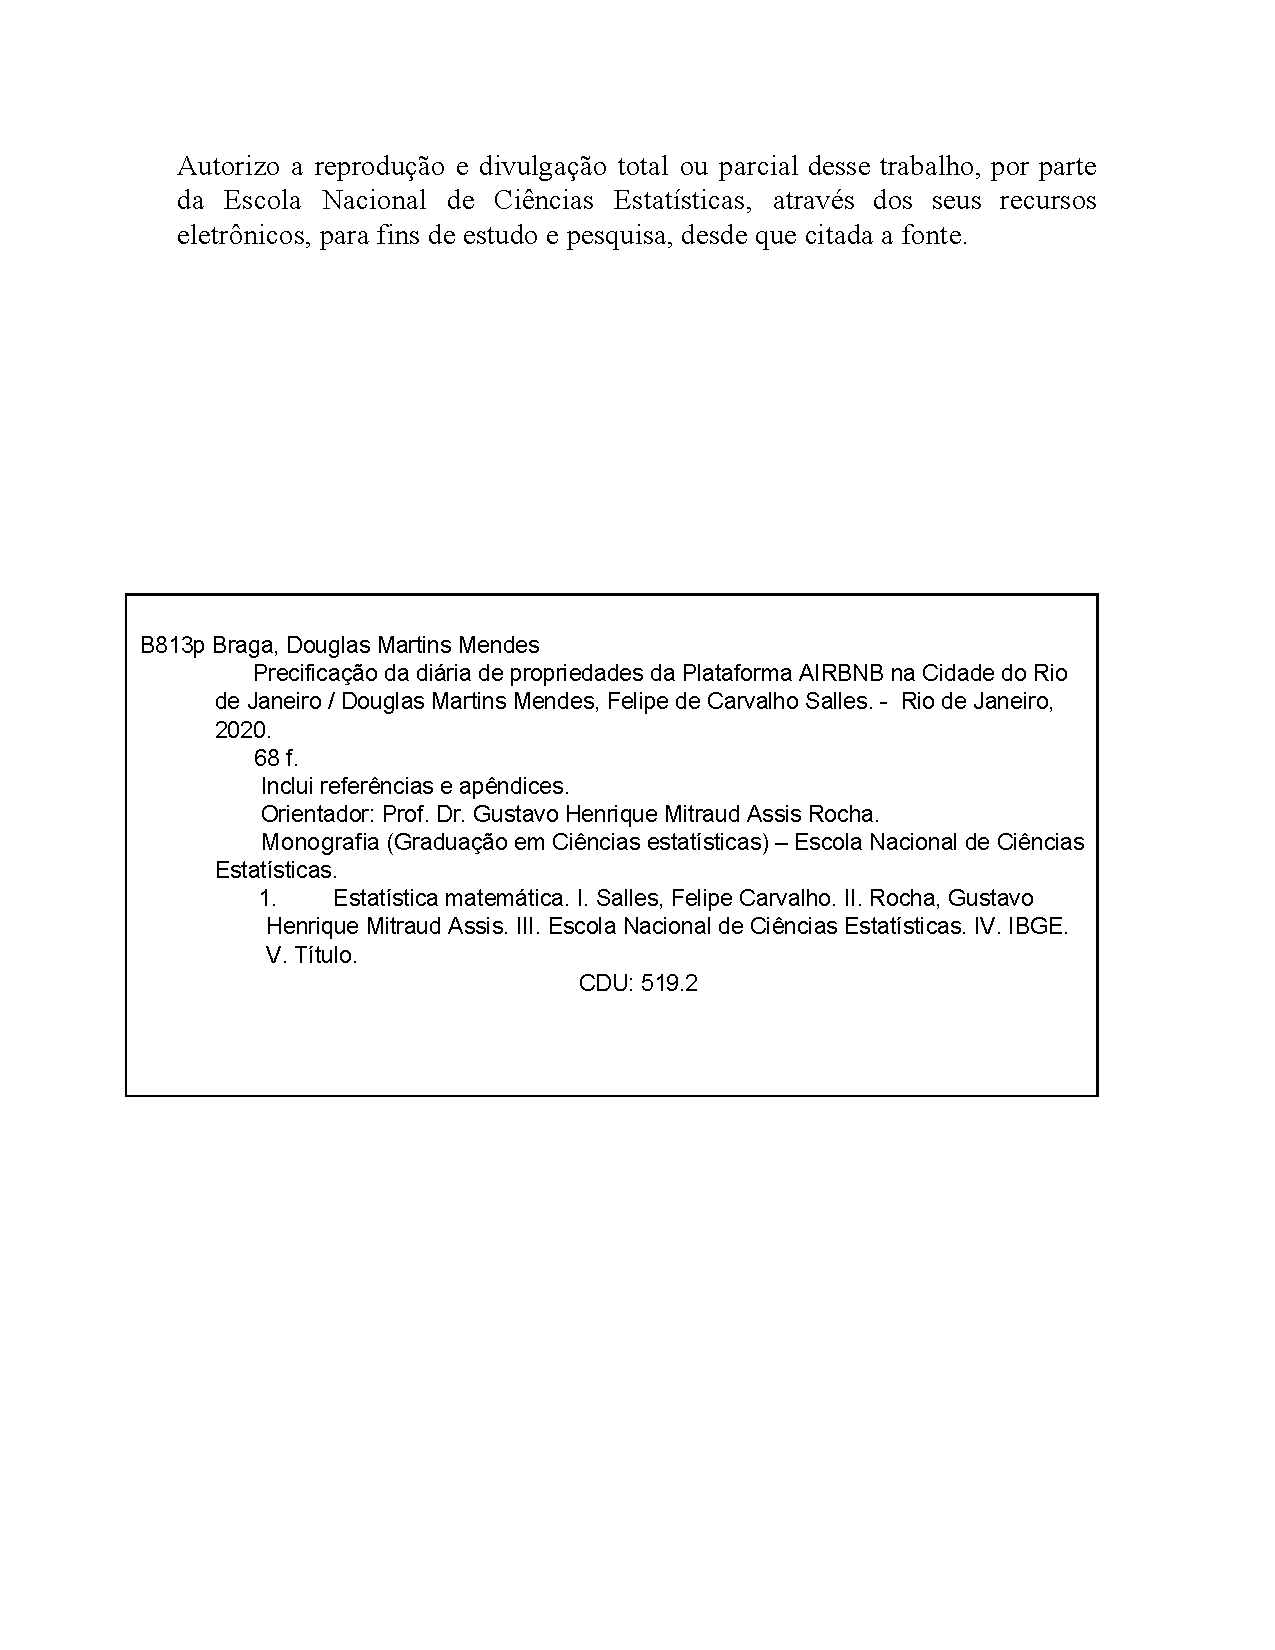
\includepdf[pages={1}]{catalografica.pdf}
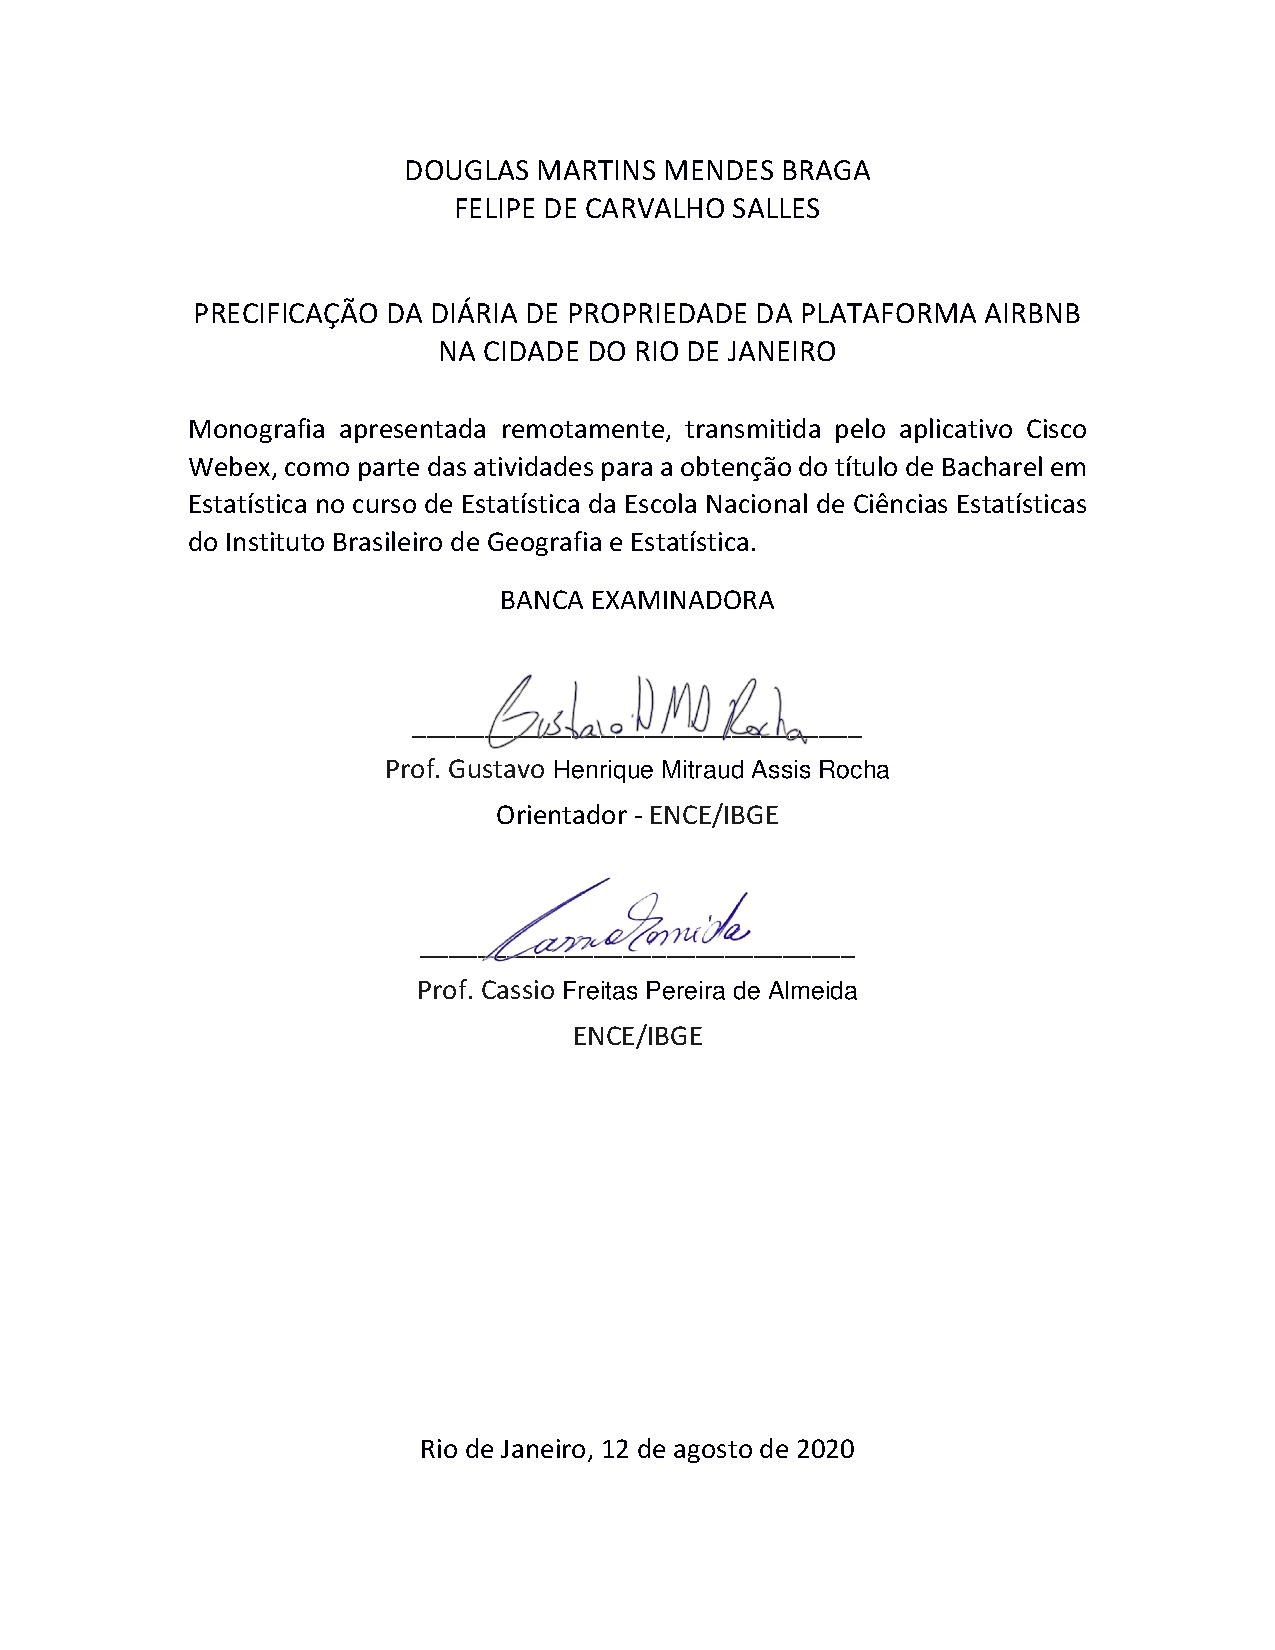
\includepdf[pages={1}]{FolhaAssinaturas.pdf}
%\imprimitfolhadeaprovacao

% ---
% Agradecimentos
% ---
\begin{agradecimentos}
	Agradecemos aos nossos familiares que nos apoiaram até aqui e que foram
a nossa fonte de inspiração. Somos gratos aos colegas de turma que
lutaram junto conosco todos os dias. Aos amigos que nunca negaram
palavras de força, incentivo e otimismo ao longo da jornada acadêmica.
Aos nossos mestres que acompanharam toda a nossa trajetória dentro do
curso de estatística. Ao nosso orientador Gustavo Rocha que foi
incansável em suas orientações, pesquisas e revisões. Nosso muito
obrigado à Escola Nacional de Ciências
Estatísticas\footnote{\url{http://www.ence.ibge.gov.br/}} por nos
proporcionar o melhor ambiente educacional.
\end{agradecimentos}
% ---

% ---
% RESUMO
% ---

% resumo na língua vernácula (obrigatório)
\setlength{\absparsep}{18pt} % ajusta o espaçamento dos parágrafos do resumo
\begin{resumo}
	A acomodação em um estabelecimento de hospedagem pode abranger uma gama
de inúmeros elementos, tais como limpeza, recepção, localização, preço e
outros. Como cada item não é comercializado separadamente no mercado,
torna-se mais complexo saber o real valor que cada um entrega ao
consumidor. Com isso, a forma de pensar e agir na definição do preço da
diária desses empreendimentos pode ter enfoque em diversas variáveis.
Esta pesquisa teve como objetivo comparar métodos de custeio do preço de
diária do site Airbnb, dos estabelecimentos localizados na cidade do Rio
de Janeiro, bem como os fatores levados em conta na formação do preço, a
fim de que o usuário possa verificar se há um preço justo na locação do
estabelecimento. A estimação dos preços foi realizada por meio de
aprendizado de máquina, com uma breve comparação a um modelo de
regressão linear. Os melhores resultados de previsão foram utlizando o
Random Forest com otimização, apresentando menores erros. Fatores
relacionados ao tamanho da propriedade foram muito relevantes neste
modelo.
	\noindent
	\\
	\\
	\textbf{Palavras-chaves}: Machine Learning. Precificação. Hospedagem
\end{resumo}
% ---

% ---
% inserir lista de ilustrações
% ---
\pdfbookmark[0]{\listfigurename}{lof}
\listoffigures*
\clearpage
% ---

% ---
% inserir lista de tabelas
% ---
\pdfbookmark[0]{\listtablename}{lot}
\listoftables*
\clearpage
% ---

% ---
% inserir lista de abreviaturas e siglas
% ---
% \begin{siglas}
%   \item[\mathcal{D}] Distribuição de Probabilidades
%   \item[\xi] Algoritmo de Aprendizado
%   \item[sign(·)] Função que retorna 1 para o caso de . > 0, -1 caso . < 0 e 0 caso . = 0
%   \item[IDH] Índice de Desenvolvimento Humano
% \end{siglas}
% ---
% ---


% ---
% inserir o sumario
% ---
\pdfbookmark[0]{\contentsname}{toc}
\tableofcontents*
\clearpage
% ---

% ----------------------------------------------------------
% ELEMENTOS TEXTUAIS
% ----------------------------------------------------------
\textual

\hypertarget{introduuxe7uxe3o}{%
\chapter{Introdução}\label{introduuxe7uxe3o}}

Nos últimos anos, um novo modelo de negócios conhecido como ``economia
compartilhada'' surgiu no setor de turismo e hospitalidade (Cohen,
\protect\hyperlink{ref-cohen2015self}{2015}; Gansky,
\protect\hyperlink{ref-gansky2010mesh}{2010}). Economia compartilhada é
um conceito extenso, em que uma de suas definições é de que se trata de
um ambiente no qual pessoas podem alugar ou emprestar bens que não estão
sendo utilizados para outros, com uma recompensa financeira. Este
modelo, não se limita apenas ao turismo, envolve diversas atividades
econômicas, sendo o turismo uma das mais relevantes (Lobo,
\protect\hyperlink{ref-loboeconomia}{2018}). O Airbnb foi precursor no
uso desse modelo de negócios para conectar pessoas que possuem ativos
ociosos de acomodação (como casas ou apartamentos) com quem precisa de
acomodação temporária (como turistas) por meio de plataformas digitais
(Botsman, \protect\hyperlink{ref-botsman2011meu}{2011}).

O crescimento exponencial da economia compartilhada envolvendo
hospedagem foi atribuído ao fornecimento de uma ampla variedade de
preços e características de propriedades, bem como uma experiência mais
diversificada do que a acomodação em um hotel tradicional (Guttentag,
\protect\hyperlink{ref-guttentag2015airbnb}{2015}; Pesonen,
\protect\hyperlink{ref-pesonen2017peer}{2017}). O preço é amplamente
reconhecido como um dos principais e mais críticos fatores que
determinam o sucesso em longo prazo da hospedagem (Hung,
\protect\hyperlink{ref-hung2010pricing}{2010}). Muitos estudos foram
realizados em estratégias de preços no setor de hospitalidade, tanto da
demanda (Becerra, \protect\hyperlink{ref-becerra2013being}{2013}; Chen e
Rothschild, \protect\hyperlink{ref-chen2010application}{2010}; Hung,
\protect\hyperlink{ref-hung2010pricing}{2010}) quanto da oferta (Huse,
\protect\hyperlink{ref-huse2006estimaccao}{2006}; Masiero,
\protect\hyperlink{ref-masiero2015demand}{2015}). Além de oferecer
produtos e serviços de qualidade com preços que o consumidor esteja
favorável a pagar, os preços devem ser suficientes para cobrir todas as
despesas. Pesquisadores anteriores ajudaram a melhorar as práticas no
setor de hospitalidade, identificando fatores determinantes das tarifas
dos quartos de hotel que influenciam na disposição dos hóspedes, e os
efeitos de diferentes estratégias de preços nas percepções e na
satisfação dos clientes (Hung,
\protect\hyperlink{ref-hung2010pricing}{2010}). No entanto, apenas
alguns pesquisadores investigaram os fatores que determinam o preço de
compartilhar acomodações baseadas na economia compartilhada (Gutt,
\protect\hyperlink{ref-gutt2015sharing}{2015}; Li,
\protect\hyperlink{ref-li2015agent}{2015}).

Com isso, o objetivo deste trabalho é aplicar modelos para compreender o
valor da diária a partir de dados da Airbnb no Rio de Janeiro. Esta
plataforma tem alcançado imensa expressividade em diversos destinos
turísticos mundiais. Com isso, houve o interesse em investigar quais
fatores influenciam nos preços de diárias de diversas propriedades,
utilizando disso para que haja uma previsão do preço final da
acomodação. Foi utilizada uma amostra de 35.793 acomodações e 116
variáveis.

No auxílio do objetivo geral, pretende-se com os objetivos específicos:

\begin{enumerate}
\def\labelenumi{\arabic{enumi})}
\item
  Examinar os dados dispostos do Airbnb;
\item
  Verificar as variáveis significativas para o julgamento do preço
  final;
\item
  Ajustar um modelo de regressão linear múltipla para predição do preço
  final da diária;
\item
  Ajustar um modelo de aprendizagem de máquina para predição do preço
  final da diária;
\item
  Comparar os modelos e verificar qual se ajusta melhor aos dados.
\end{enumerate}

Este trabalho está organizado da seguinte forma:

\begin{itemize}
\tightlist
\item
  Capítulo 1: introdução ao tema.
\item
  Capítulo 2: revisão bibliográfica do tema.
\item
  Capítulo 3: metodologia de coleta e informações gerais das bases de
  dados.
\item
  Capítulo 4: metodologia utilizada no trabalho.
\item
  Capítulo 5: resultados.
\end{itemize}

Por fim, no apêndice é apresentado todo o script utilizado no software
estatístico para manipulação, tratamento e análise dos dados.

\hypertarget{revisuxe3o-bibliogruxe1fica}{%
\chapter{Revisão Bibliográfica}\label{revisuxe3o-bibliogruxe1fica}}

Um novo movimento, chamado de \emph{economia compartilhada}, apareceu há
pouco tempo como uma opção para atender necessidades diversas, que,
anteriormente, eram satisfeitas dominantemente por empresas. Os clientes
passaram a querer ter acesso a produtos e a pagar pela experiência de
tê-los momentaneamente, ao invés de adquiri-los por definitivo
(Eckhardt, \protect\hyperlink{ref-eckhardt2015sharing}{2015}).

Segundo Belk (\protect\hyperlink{ref-belk2014you}{2014}), a economia
compartilhada é o resultado da progressão tecnológica e socioeconômica.
O rápido desenvolvimento da tecnologia com relação à informação e
comunicação, tanto por parte de hardwares (como por exemplo, smartphones
e tablets) quanto softwares (como por exemplo, aplicativos), concedeu
aos usuários promover seu próprio conteúdo, compartilhar informações,
colaborar e realizar transações por meio de plataformas (Kaplan,
\protect\hyperlink{ref-kaplan2010users}{2010}).

Logo, a economia compartilhada baseada em diversos modelos de negócios
foram rapidamente adotados em várias áreas, como aluguel de ativos
próprios (Airbnb.com para acomodações e Moobie.com.br para carros),
trabalho autônomo de forma provisória (por exemplo, Fiverr.com), entre
outros (Sundararajan,
\protect\hyperlink{ref-sundararajan2014peer}{2014}). Lavaquial
(\protect\hyperlink{ref-lavaquial2015cocriando}{2015}) acrescenta ainda
que esta nova modalidade de negócios conecta a oferta com a demanda, sem
necessidade de intermediário, sendo a tecnologia um dos fatores
impulsionadores e característicos de práticas colaborativas.

A diversidade de sites para aluguel de acomodações, considerando a
economia compartilhada, experimentou um crescimento fenomenal devido à
alta demanda turística (Guttentag,
\protect\hyperlink{ref-guttentag2015airbnb}{2015}; Heo,
\protect\hyperlink{ref-heo2016sharing}{2016}; Karlsson,
\protect\hyperlink{ref-karlsson2016someone}{2016}; Tussyadiah,
\protect\hyperlink{ref-tussyadiah2016strategic}{2016}). Esse tipo de
hospedagem é oferecido nos mercados digitais (por exemplo, Airbnb.com e
HomeAway.com) por pessoas que possuem o direito de usar o espaço
fornecido (Guttentag, \protect\hyperlink{ref-guttentag2015airbnb}{2015};
Heo, \protect\hyperlink{ref-heo2016sharing}{2016}).

Há a possibilidade de acesso a serviços mais baratos e, não por isso,
menos qualificados que o hotel, porém de forma privada, representando um
novo modo de relação interpessoal (Botsman,
\protect\hyperlink{ref-botsman2010s}{2010}). Turistas relatam diversos
benefícios na hospedagem no modelo de economia compartilhada, como
benefício principal a redução de custos, além da oportunidade de
intercâmbio e interação social com seus anfitriões (que podem ser
residentes locais) (Balck,
\protect\hyperlink{ref-balck2015empirical}{2015}; Guttentag,
\protect\hyperlink{ref-guttentag2015airbnb}{2015}; Quinby,
\protect\hyperlink{ref-quinby2014share}{2014}). Sendo assim, a suposição
que temos é que o preço é considerado um dos fatores mais relevantes
para o consumidor para o uso destas plataformas.

Airbnb, ``um dos maiores mercados do mundo para estadias e atividades
únicas e
autênticas''\footnote{\url{https://news.airbnb.com/br/about-us/}}, é a
plataforma líder para o modelo de negócios de hospedagem da economia
compartilhada. Fundado em 2008 por Brian Chesky e Joe Gebbia, o
Airbnb.com oferece mais de sete milhões de acomodações em mais de 220
países e regiões.

A literatura sobre preço é bastante diversificada. Para Woodruff
(\protect\hyperlink{ref-woodruff1997customer}{1997}), o conceito de
valor dá-se exclusivamente à definição pelo cliente, sobre as
preferências e as avaliações das características do produto, do
desempenho dessas particularidades e das consequências originadas pelo
uso, enquanto que para Horngren
(\protect\hyperlink{ref-horngren2008contabilidade}{2008}), a oferta e
procura ditam a definição do preço de um produto ou serviço. As três
influências que incidem sobre ``oferta e procura'' são: os custos, os
concorrentes e os clientes. Os clientes influenciam a formação dos
preços na medida em que analisam o valor cobrado pelo bem ou serviço e
os benefícios que poderão vir a ter se adquiri-los. Os consumidores
consideram suas preferências em termos dos benefícios recebidos pelo
preço pago. Dessa forma, serviços e bens semelhantes tendem a ter preços
semelhantes.

Para Kotler (\protect\hyperlink{ref-kotler2007principios}{2007}), no
final das contas, é o consumidor quem irá decidir se o preço de um
produto está correto. Em todo caso, o melhor não é cobrar preços mais
baixos, mas diferenciar o produto ofertado para que ele valha um preço
mais alto, de acordo com suas características. Segundo Baker
(\protect\hyperlink{ref-baker2005administraccao}{2005}), o preço está
fortemente relacionado ao volume de vendas e atuação no mercado,
desempenhando uma forte motivação à demanda.

Com relação ao preço de se hospedar em algum tipo de acomodação do
Airbnb, há alguns estudos na literatura que mostram, por exemplo, que
propriedades com melhores avaliações cobrarem preços mais altos (Gutt,
\protect\hyperlink{ref-gutt2015sharing}{2015}; Ikkala,
\protect\hyperlink{ref-ikkala2014defining}{2014}). Para Tang
(\protect\hyperlink{ref-tang2015neighborhood}{2015}) há uma interação
entre localização e preço, relacionada a uma pesquisa com base em
propriedades no Airbnb de São Francisco.

Esses estudos iniciaram um interesse em examinar os fatores que
determinam o preço da diária baseada na economia compartilhada na cidade
do Rio de Janeiro, com objetivo na predição do mesmo. Na formação dos
preços de serviços há vários métodos e estratégias que podem ser
empregados ligados às condições do mercado, avaliações, às necessidades
dos consumidores, a concorrência, características do imóvel, aos custos
e ao retorno esperado. Para não ter sua empresa fora do mercado, o
gestor deve conceber uma boa ferramenta para a definição do preço.

Nesse sentido, na sequência faz-se um modelo baseado em aprendizado de
máquina e outro baseado em uma regressão linear, sobre a formação de
preços com base em: custos, localização, índices, valor percebido, entre
outros, de modo que o consumidor possa analisar serviços similares e/ou
substitutos, e identificar a percepção de valor dos clientes em relação
a hospedagem oferecida. Isso auxiliará na definição de preço justo. Com
isso, faremos a comparação do desempenho preditivo de um modelo de
regressão mais simples com o modelo de aprendizado de máquina e
verificar o quanto é necessário um modelo mais complexo.

\hypertarget{base-de-dados}{%
\chapter{Base de Dados}\label{base-de-dados}}

Para este trabalho, foram utilizadas três bases de dados, duas com a
origem do site Airbnb
(\protect\hyperlink{ref-inside}{2020}\protect\hyperlink{ref-inside}{a})
que, além de disponibilizar uma base com as informações das locações,
também disponibiliza um arquivo no formato \emph{geojson}, que fornece
os limites dos bairros somente para a cidade do Rio de Janeiro, como
pode ser visto na Figura \ref{mapa_bairro}.

\begin{figure}
\centering
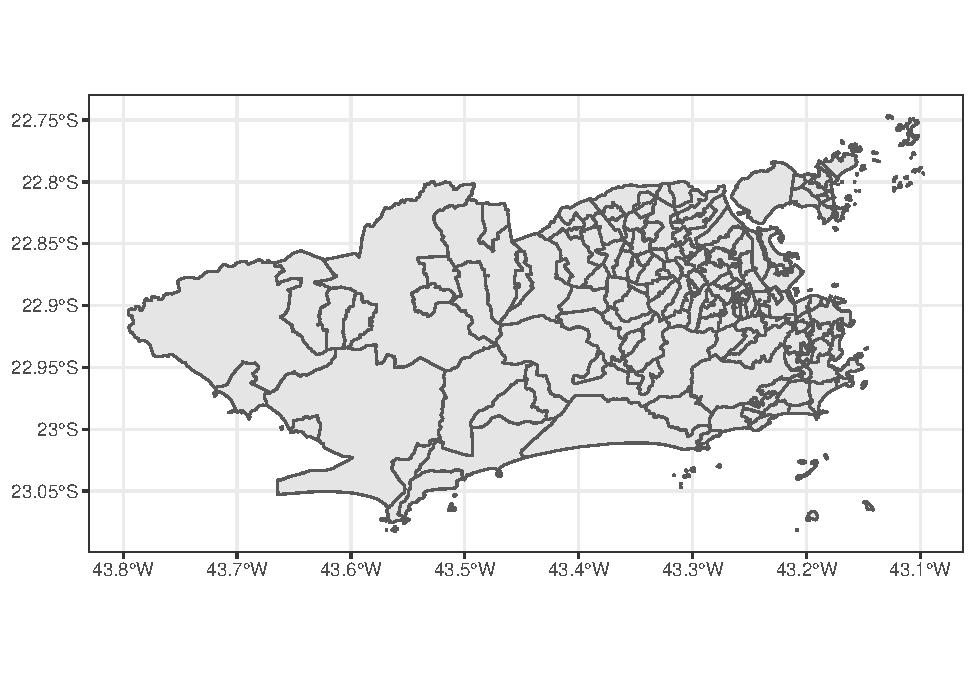
\includegraphics{00-TCC_files/figure-latex/unnamed-chunk-7-1.pdf}
\caption{\label{mapa_bairro}Limite dos bairros do Rio de Janeiro}
\end{figure}

O Inside Airbnb é um conjunto independente de recursos e dados não
comerciáveis que permite conhecer como o Airbnb está realmente sendo
usado nas diversas cidades do mundo.

Ao analisar informações publicamente disponíveis sobre as propriedades
listadas do Airbnb de uma cidade, o Inside Airbnb fornece filtros e
métricas importantes para que você possa ver como o Airbnb está sendo
usado para competir com o mercado imobiliário residencial. Com o Inside
Airbnb, há a possibilidade de se fazer questionamentos tantos básicos
quanto avançados sobre o Airbnb em qualquer lugar, restringindo até
mesmo por bairros como, por exemplo:

\begin{itemize}
\item
  ``Quantas locações existem próximas de mim?''
\item
  ``Quantas casas e apartamentos estão sendo alugados com frequência
  para turistas e não para residentes de longa duração?''
\item
  ``Quanto os anfitriões ganham com aluguel para turistas?''
\end{itemize}

A terceira base de dados se trata de variáveis fornecidas pelo site
Data.RIO (\protect\hyperlink{ref-datario}{2020}) que foi utilizada para
enriquecimento da base de dados com informações que podem ajudar
precificação de diárias, faz parte de um projeto pioneiro do Instituto
Pereira Passos (IPP) na transparência e desenvolvimento de informações
estatísticas, mapas, estudos e pesquisas com foco na Cidade do Rio de
Janeiro. Neste trabalho utilizou-se variáveis como esperança de vida,
taxa de alfabetização, frequência escolar, renda per capita, índice de
desenvolvimento humano (IDH), separadas por bairros, do ano de 2000,
para verificar se há influência de áreas melhor desenvolvidas com o
valor cobrado da diária.

\hypertarget{metodologia}{%
\chapter{Metodologia}\label{metodologia}}

Neste capítulo são descritos aspectos metodológicos para a realização do
trabalho. É apresentado o modelo de Regressão Linear Múltipla e o
algoritmo Random Forest, que é um algoritmo de aprendizado de máquina
baseado em \emph{ensemble}, além de técnicas estatísticas para a
obtenção de novas variáveis e melhorias do modelo.

\hypertarget{aprendizado-supervisionado}{%
\section{Aprendizado Supervisionado}\label{aprendizado-supervisionado}}

O método de aprendizado supervisionado necessita de um conjunto de
variáveis independentes \((X_1, X_2, X_3, ...)\), que devem possuir
alguma influência em uma ou mais variáveis que podem ser chamadas de
variáveis dependentes ou variáveis respostas \((Y_1,Y_2,Y_3,...)\)
(Friedman, \protect\hyperlink{ref-friedman2001elements}{2001}). Este
trabalho, por exemplo, tem como interesse utilizar como variáveis
independentes algumas medidas de locações disponíveis no site Airbnb
para predizer o preço da diária, sendo assim, tem-se a equação:

\[
Y = f(\boldsymbol{X}) + \epsilon,
\]

\noindent onde \(f(.)\) é uma função desconhecida, \(\epsilon\) é um
erro aleatório com média zero e variância \(\sigma^2\) e
\(\boldsymbol{X}\) o conjunto das variáveis independentes
\((X_1, X_2, X_3, ...)\).

Os modelos supervisionados têm como objetivo utilizar uma amostra de
\(\boldsymbol{X}\) e \(Y\) conhecidos para encontrar \(\hat{f}\), uma
estimativa da função desconhecida \(f\).

\hypertarget{avaliauxe7uxe3o-de-modelos}{%
\subsection{Avaliação de Modelos}\label{avaliauxe7uxe3o-de-modelos}}

Para a definição da métrica de erro que será utilizada para a avaliação
do modelo, primeiro é necessário definir o tipo de problema a ser
resolvido, sendo um problema de regressão ou de classificação. Essa
definição é feita por meio da observação da variável resposta. Tendo a
métrica de erro definida, é possível realizar a estimativa da função
\(f\) e encontrar uma estimativa da variável resposta
\(\hat{Y} = \hat{f}(\boldsymbol{X})\) e com isso mensurar o erro do
modelo.

Este trabalho será baseado em um problema do tipo regressão, onde \(Y\)
é uma variável contínua.

Uma forma de testar a estimativa da função \(f\) é realizar uma amostra
das observações (linhas) da base de dados, e com isso separar em dois
conjuntos \((Y_o, \boldsymbol{X_0})\) e \((Y_1, \boldsymbol{X_1})\),
onde uma parte será utilizada para estimar a função e outra para testar
essa estimativa. Além disto, pode ser útil para identificar o
sobreajuste do modelo/algoritmo, um problema que ocorre onde o
modelo/algoritmo fica superajustado a base de treino e perde o poder de
generalização.

Serão utilizados quatro critérios para avaliar a qualidade preditiva de
um modelo/algoritmo de previsão, que são: Erro Quadrático Médio (EQM),
Raiz do Erro Quadrático Médio (REQM), Erro Absoluto Médio (EAM) e Erro
Percentual Absoluto Médio (EPAM). Essas métricas são úteis para comparar
diferentes métodos aplicados ao mesmo conjunto de dados.

\begin{itemize}
\tightlist
\item
  Erro quadrático médio
\end{itemize}

O erro quadrático médio (EQM), traduz o valor médio dos desvios ao
quadrado entre os valores observados e as previsões para as observações
\(1, 2,\dots,n\), ou seja,

\[EQM = \frac{1}{n}\sum_{i=1}^n(Y_i - \hat{Y}_i)^2.\]

\begin{itemize}
\tightlist
\item
  Raiz do Erro Quadrático Médio
\end{itemize}

Muitas vezes, a raiz do erro quadrático médio é preferida ao EQM porque
permite reduzir a grandeza dos valores para a mesma escala dos dados,
definida como:

\[REQM = \sqrt{EQM}.\]

\begin{itemize}
\tightlist
\item
  Erro Absoluto Médio
\end{itemize}

Historicamente, a REQM e o EQM são medidas bastante utilizadas. No
entanto, estas medidas são mais sensíveis a outliers do que outras do
mesmo tipo, como, por exemplo, o erro absoluto médio, que se define
como:

\[EAM = \frac{1}{n} \sum_{i=1}^n |Y_i - \hat{Y}_i|.\]

\begin{itemize}
\tightlist
\item
  Erro Percentual Absoluto Médio
\end{itemize}

O erro percentual absoluto médio, EPAM, representa a percentagem média
do erro de previsão em relação à grandeza das observações, sendo,
portanto, uma medida de erros percentuais, que se define como:

\[EPAM =  \frac{1}{n} \sum_{i=1}^n \left| \frac{Y_i - \hat{Y}_i}{Y_i} \right|.\]

\hypertarget{validauxe7uxe3o-cruzada}{%
\subsection{Validação cruzada}\label{validauxe7uxe3o-cruzada}}

Como citado anteriormente, será utilizada a separação da base de dados
para o treinamento e teste do modelo. Na maioria de modelos/algoritmos
de aprendizagem de máquina, há parâmetros que precisam ser informados
antes do treinamento. Essas informações são chamadas de hiperparâmetros.
Com isso, existe o problema de escolher um bom conjunto de
hiperparâmetros para um algoritmo de aprendizagem, por isso é necessário
uma otimização manual, onde busca-se otimização dos erros (detalhados
posteriormente).

Para isso, será utilizada a técnica de validação cruzada, que consiste
em separar a base de treino em \(K\) partes, onde serão realizadas \(K\)
rodadas, onde na rodada \(T\) a parte \(T\) será utilizada para testar o
modelo e as demais partes serão utilizadas para o treinamento de um
modelo, esse algoritmo é representado na Figura \ref{img:kfold}.

\begin{figure}
\centering
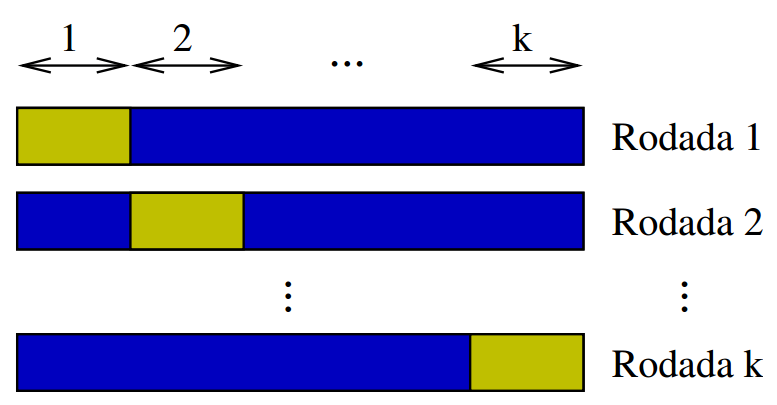
\includegraphics[width=\textwidth,height=0.4\textheight]{../fig/kfold.png}
\caption{\href{https://pt.stackoverflow.com/questions/66777/d\%C3\%BAvidas-na-utiliza\%C3\%A7\%C3\%A3o-de-stratified-k-fold-no-scikit-learn}{Exemplo
de validação cruzada.\label{img:kfold}}}
\end{figure}

Resumidamente, para cada teste de hiperparâmetro teremos \(K\)
avaliações e com isso é possível ter uma ideia do poder preditivo da
função estimada (\(\hat{f}\)) e também de sua variabilidade. Com a
validação cruzada podemos testar vários cenários antes de colocarmos o
nosso modelo em produção e avaliar a capacidade de generalização de um
modelo.

\hypertarget{regressuxe3o-linear-muxfaltipla}{%
\subsection{Regressão Linear
Múltipla}\label{regressuxe3o-linear-muxfaltipla}}

Tem-se uma regressão linear múltipla quando se admite que a variável
resposta (Y) é função de duas ou mais variáveis explicativas
(regressoras). Sejam \(X_1\),\(X_2\), \(\dots\) , \(X_p\) as p variáveis
explicativas relacionadas à variável resposta Y e \(x_{n,1}\),
\(x_{n,2}\), \(\dots\), \(x_{n,p}\) valores observados das variáveis
explicativas (constantes conhecidas) (Neter,
\protect\hyperlink{ref-neter1989applied}{1989}). Especificamente, o
modelo de regressão linear fica na forma:

\[
Y_i = \beta_0 + \beta_1 X_{i1} + \beta_2 X_{i2}+\dots + \beta_p X_{ip} + \epsilon_i
\]

Em notação matricial, podemos escrever o modelo da seguinte forma:

\[
\begin{bmatrix}
Y_1 \\
Y_2 \\
\vdots \\
Y_n
\end{bmatrix}
=
\begin{bmatrix}
1 & x_{1,1} & x_{1,2} & \dots & x_{1,p} \\
1 & x_{2,1} & x_{2,2} & \dots & x_{2,p} \\
\vdots & \vdots & \vdots & \ddots & \vdots \\
1 & x_{n,1} & x_{n,2} & \dots & x_{n,p}
\end{bmatrix}
\begin{bmatrix}
\beta_0 \\
\beta_1 \\
\vdots \\
\beta_n
\end{bmatrix}
+
\begin{bmatrix}
\epsilon_1 \\
\epsilon_2 \\
\vdots \\
\epsilon_n
\end{bmatrix}
\]

ou

\[
\begin{matrix}
\underbrace{\textbf{Y}}_{(n\times 1)} 
= 
\underbrace{\textbf{X}}_{n\times(p+1)}
\underbrace{\theta}_{(p+1)\times1}
+
\underbrace{\underline{ \epsilon}}_{(n\times 1)}
\end{matrix}
\]

em que:

\begin{itemize}
\item
  \(\textbf{Y} = (Y_1,\dots , Y_n)^T\) : o vetor transposto das
  observações da variável aleatória Y.
\item
  \(\textbf{X}\): matriz dos valores constantes de x observados para
  cada observação da reposta y.
\item
  \(\theta\): vetor dos coeficientes do modelo.
\item
  \(\underline{ \epsilon}\): vetor dos erros aleatórios.
\end{itemize}

Além disso, têm-se as suposições:

\begin{enumerate}[label=(\roman*)]
\item a variável resposta Y tem relação linear com as variáveis explicativas $X_j$, j = 1, 2,$\dots$, p;
\item as variáveis explicativas $X_j$ são conhecidas;
\item $E(\epsilon_i)$ = 0, ou seja, $E(\underline{ \epsilon}) = \textbf{0}$, sendo $\textbf{0}$ um vetor de zeros de dimensões $n \times 1$;
\item os erros são homocedásticos, isto é, Var($\epsilon_i$) = E($\epsilon_i^2$) = $\sigma^2$;
\item os erros são independentes, isto é, Cov($\epsilon_i,\epsilon_{j}$) = E($\epsilon_i \epsilon_{j}^T$) = 0, i $\neq$ j;
\item os erros têm distribuição normal.
\end{enumerate}

Logo, combinando-se (iv) e (v) tem-se Var(\(\underline{ \epsilon}\)) =
E(\(\underline{ \epsilon} \underline{ \epsilon}^T\)) =
\(\textbf{I}\sigma^2\), sendo \(\textbf{I}\) uma matriz identidade, de
dimensão \(n \times n\). Portanto, considerando-se, também, (vi) tem-se
\(\underline{ \epsilon} \sim N(\textbf{0},\textbf{I}\sigma^2)\) e
\(\textbf{Y} \sim N(\textbf{X}\theta, \textbf{I}\sigma^2)\), pois,
\(E(\textbf{Y}) = \textbf{X}\theta\) e
Var(\(\textbf{Y}) = Var(\underline{ \epsilon}) = \textbf{I}\sigma^2\). A
suposição de normalidade é necessária para a elaboração dos testes de
hipóteses para os coeficientes do modelo.

Haverá um resíduo
\(\hat{\epsilon}_i = y_i - \hat{y}_i = y_i - (\hat{\beta}_0 + \hat{\beta}_1x_{1,i} + \hat{\beta}_2x_{2,i} + \dots + \hat{\beta}_px_{p,n})\),
onde \(\hat{y}_i\) é a estimativa de \(y_i\) e \(\hat{\beta_i}\) o
coeficiente \(\beta_i\) estimado, com \(i = 0,1,\dots , p\). O vetor de
resíduos
\(\underline{\hat{\epsilon}} = \textbf{Y} - \textbf{X}\hat{\theta}\)
contém informação sobre o parâmetro desconhecido \(\sigma^2\). Estima-se
os parâmetros \(\beta_0,\beta_1,\dots,\beta_p\) de modo a minimizar a
soma dos quadrados dos erros, dada por:

\[SQR = \sum_{i=1}^n \hat{\epsilon}^2_i = \sum_{n=1}^n (y_i- \hat{\beta_0} - \hat{\beta}_1x_{1,i} - \hat{\beta}_2x_{2,i}- \dots - \hat{\beta}_px_{p,i})^2.\]

Assumindo que a matriz \(X^TX\) é não singular, a solução do sistema é:

\[
\hat{\beta}
=
\begin{bmatrix}
\hat{\beta_0} \\
\hat{\beta_1} \\
\vdots \\
\hat{\beta_p}
\end{bmatrix}
=
(X^TX)^{-1}X^TY
\]

que é estimativa para:

\[
\beta =
\begin{bmatrix}
\beta_0 \\
\beta_1 \\
\vdots \\
\beta_p
\end{bmatrix}
\]

A medida \(R^2\) de ajuste é baseada na soma dos quadrados total
(\(SQT\)) e na soma dos quadrados dos resíduos (\(SQR\)), que pode ser
interpretada como o percentual de variabilidade que o modelo explica,
definida como:

\[
R^2 = 1-\frac{SQR}{SQT}
\]

\noindent onde, \(SQT=\sum_{i=1}^n(y_i-\bar{y})\), e \(\bar{y}\) é a
média amostral de \(y_i\), .

No presente trabalho foi utilizada a técnica de regressão linear
múltipla para ajustar um modelo de previsão em que a variável resposta é
o valor da diária da propriedade. Para tal, utilizamos diversas técnicas
para atingir os pressupostos do modelo, além de deixá-lo mais
parcimonioso com um menor erro de predição, como é no caso da regressão
de LASSO detalhada mais a frente.

\hypertarget{transformauxe7uxe3o-box-cox}{%
\subsubsection{Transformação
Box-Cox}\label{transformauxe7uxe3o-box-cox}}

Conforme já foi visto, o modelo linear clássico é válido sob as
seguintes pressuposições:

\begin{enumerate}[label=(\roman*)]
\item simplicidade de estrutura para o valor esperado da variável resposta (aditividade do modelo);
\item independência e homogeneidade dos erros;
\item normalidade dos erros.
\end{enumerate}

Se não for possível satisfazer a esses requisitos na escala original dos
dados, pode ser que uma transformação não linear dos dados possa
produzir homogeneidade de variâncias e distribuição aproximadamente
normal. Em simples palavras, significa que precisamos montar um gráfico
com os dados para verificar o comportamento da distribuição subjacente.
Com o gráfico, às vezes também descobrimos que uma pequena transformação
resulta em um comportamento aproximado de uma distribuição normal. Isso
significa que as transformações de dados podem simplificar nossa vida e
nos permitem usar medidas estatísticas destinadas a dados normalmente
distribuídos.

Box (\protect\hyperlink{ref-box1964analysis}{1964}) propuseram uma
família de transformações dada por:

\[Y(\lambda)
= \left\{ \begin{array}{rll}
\frac{Y^{\lambda}-1}{\lambda} & \hbox{se} & \lambda \neq 0 \\
\log(Y) & \hbox{se} & \lambda = 0
\end{array}\right.\]

\noindent onde \(\lambda\) o parâmetro da transformação e Y uma variável
aleatória. Na ausência de uma transformação, \(\lambda\)= 1.

O objetivo da transformação é determinar \(\lambda\) (ou uma escala para
Y), tal que sejam verdadeiras as pressuposições citadas no inicio desta
seção.

Cabe ressaltar que tal transformação não se limita à variável resposta,
porém neste trabalho foi utilizada para contornar o problema de
distribuição assimétrica da variável resposta.

\hypertarget{regularizauxe7uxe3o}{%
\subsubsection{Regularização}\label{regularizauxe7uxe3o}}

Segundo Friedman (\protect\hyperlink{ref-friedman2001elements}{2001}), a
seleção de um subconjunto de variáveis produz um modelo que é
interpretável e, possivelmente, possui um erro de previsão menor do que
o modelo completo. Quando se tem muitas variáveis explicativas, faz-se
necessário selecionar as que resultariam em um modelo útil e
parcimonioso. Uma solução para isso pode ser utilizar a técnica de
regularização LASSO, método pelo qual as estimativas dos coeficientes
menos relacionados a variável resposta tendem a zero, o que implica que
apenas as variáveis que afetam significativamente a variação em Y sejam
consideradas no modelo. Os métodos de regularização mais comuns são
LASSO (\(\ell_1\)), Ridge (\(\ell_2\)) e a mistura dos dois
(\emph{elastic net}).

O LASSO é indiferente quanto aos regressores correlacionados e tenderá a
escolher um e ignorar os demais, enquanto o Ridge reduz os coeficientes
regressores relacionados uns em relação aos outros, ambos impondo
diferentes penalidades em seu tamanho. LASSO também é amplamente
utilizado para seleção de variáveis.

\hypertarget{regressuxe3o-lasso}{%
\paragraph{Regressão LASSO}\label{regressuxe3o-lasso}}

O LASSO é uma metodologia proposta por Tibshirani
(\protect\hyperlink{ref-tibshirani1996regression}{1996}), cujo
significado é \emph{Least Absolute Shrinkage and Selection} (``menor
encolhimento absoluto e seleção''). Os estimadores dos parâmetros do
LASSO são dados pela resolução do seguinte problema:

\[
\hat{\beta}^{LASSO} =\underset{\beta}{argmin}  \sum_{i=1}^N \left( y_i-\beta_0 -\sum_{j=1}^p x_{ij} \beta_j\right)^2 \hbox{sujeito a } \sum_{j=1}^p|\beta_j|\leq t,
\]

\noindent no qual \(\hat{\beta}^{LASSO}\) é o vetor de coeficientes de
regressão associados às variáveis (incluindo o intercepto \(\beta_0\)).
O parâmetro \(t\geq0\) controla o encolhimento (redução) do modelo, isto
é, reduzindo o número de variáveis regressoras ao qual o
\(\hat{\beta_i}\) associado é zero.

Também pode-se escrever o problema do LASSO na forma de Lagrange:

\[\hat{\beta}^{LASSO}=\underset{\beta}{argmin} \left\{ \frac{1}{2} \sum_{i=1}^N \left( y_i-\beta_o-\sum_{j=1}^px_{ij}\beta_j \right)^2 + \lambda\sum_{j=1}^p|\beta_j| \right\},\]

\noindent onde \(\lambda\), de forma similar a \(t\), controla o
encolhimento (redução) do modelo.

O parâmetro \(\lambda\) controla a força da penalização, onde torná-lo
suficientemente grande faz com que mais coeficientes sejam reduzidos a
zero, utilizando \(\lambda=0\) temos a regressão linear múltipla padrão,
sem penalização. O valor de \(\lambda\) deve ser escolhido de forma
adaptativa para minimizar uma estimativa de erro esperado de previsão. O
autor propõe que se utilize de métodos de validação cruzada para
escolher o parâmetro \(\lambda\), consistindo em uma aproximação linear
do LASSO, com detalhes em Friedman
(\protect\hyperlink{ref-friedman2001elements}{2001}).

\hypertarget{muxe9todos-ensemble}{%
\subsection{Métodos Ensemble}\label{muxe9todos-ensemble}}

Muitos pesquisadores buscam maneiras de combinar a previsão de diversos
modelos para criar um único modelo que possua uma taxa de acertos maior
(Opitz, \protect\hyperlink{ref-opitz1999popular}{1999}). Os dois
principais algoritmos que atendem esse objetivo são: \emph{bootstrap
aggregating} (Breiman, \protect\hyperlink{ref-breiman1996bagging}{1996})
e \emph{boosting} (Schapire,
\protect\hyperlink{ref-schapire1999brief}{1999}). Ambos os algoritmos
utilizam um modelo base como regressão logistica (Friedman,
\protect\hyperlink{ref-friedman2000additive}{2000}), árvores de decisão,
redes neurais (Martínez-Muñoz,
\protect\hyperlink{ref-martinez2019sequential}{2019}), e qualquer outro
modelo de aprendizagem supervisionada.

\hypertarget{bootstrap}{%
\subsubsection{Bootstrap}\label{bootstrap}}

O procedimento Bootstrap é uma técnica de reamostragem, bastante
utilizada em diferentes situações estatísticas. A base da técnica é a
obtenção de um ``novo'' conjunto de dados, por reamostragem do conjunto
de dados original. O aumento de poder computacional estimulou o
desenvolvimento de novos métodos estatísticos que são computacionalmente
intensivos, como o próprio bootstrap introduzido por Efron
(\protect\hyperlink{ref-efron1994introduction}{1994}). O objetivo é a
estimativa de um parâmetro da população como pode ser visto na Figura
\ref{fig:bootstrap}. O procedimento é útil nos casos em que o estimador
é uma função complexa dos parâmetros verdadeiros (Murphy,
\protect\hyperlink{ref-murphy2012probabilistic}{2012}).

Numa análise, normalmente, temos uma amostra de uma população do
interesse no estudo. A análise é realizada nesta amostra. Utilizando o
bootstrap, é feito uma amostragem aleatória com reposição dessa amostra
e simulando diversas outras possíveis amostras que poderiam ser
retiradas da população.

\begin{figure}
\centering
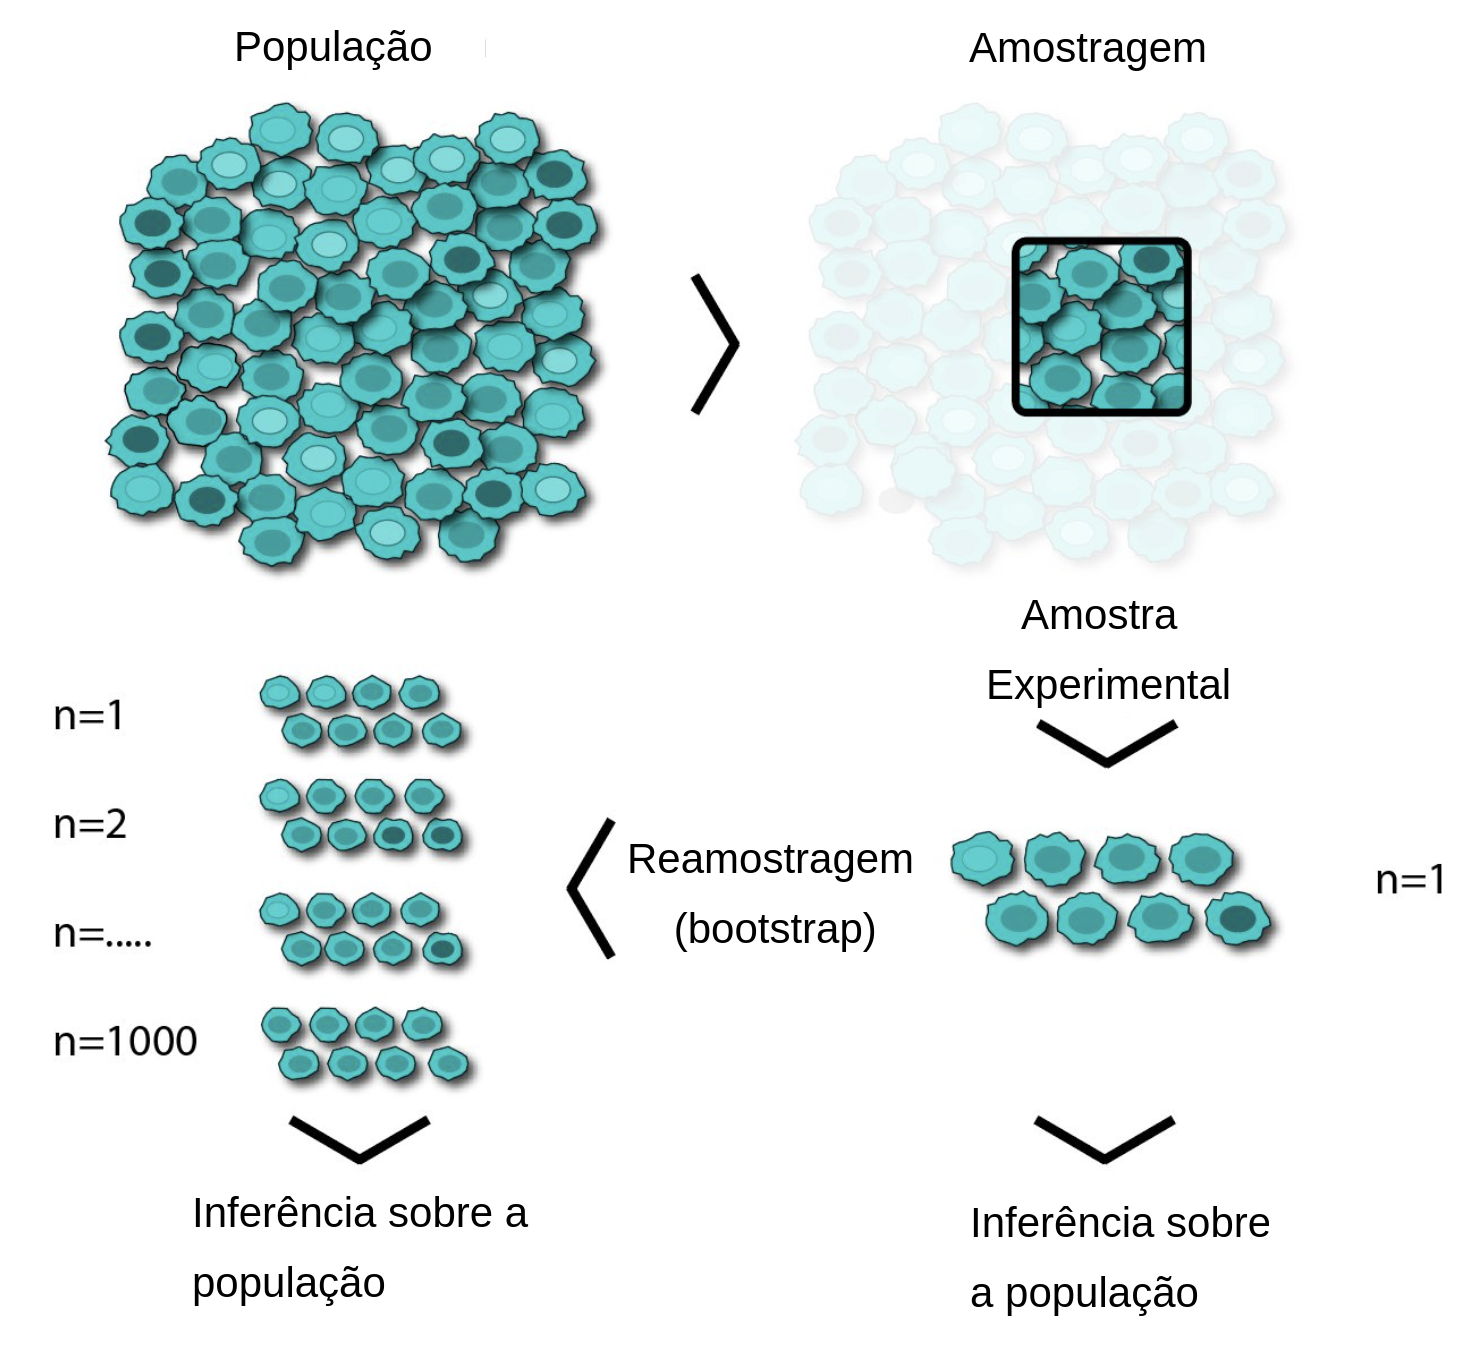
\includegraphics[width=\textwidth,height=0.4\textheight]{../fig/bootstrap_traduzido.png}
\caption{Exemplo de bootstrap.\label{fig:bootstrap}}
\end{figure}

\hypertarget{uxe1rvore-de-decisuxe3o}{%
\subsubsection{Árvore de decisão}\label{uxe1rvore-de-decisuxe3o}}

O sucesso dos algoritmos de árvores de decisão é explicado por vários
fatores que os tornam bastante atraentes na prática:

\begin{itemize}
\tightlist
\item
  As árvores de decisão são não-paramétricas. Eles podem modelar
  arbitrariamente relações complexas entre variáveis explicativas e
  variável resposta, sem qualquer suposição a priori;
\item
  Facilidade em lidar com dados heterogêneos (variáveis ordenadas ou
  categóricas ou uma mistura de ambas);
\item
  Implementação intrínseca na seleção de variáveis;
\item
  As árvores de decisão são robustas para discrepâncias ou erros nos
  rótulos;
\item
  As árvores de decisão são facilmente interpretáveis.
\end{itemize}

Existem diversos algoritmos relacionados a árvores de decisão, variando
a forma que é feita a seleção das variáveis, dos pontos de divisão,
entre outros. Um dos algoritmos mais utilizados é o algoritmo
\emph{classification and regression trees (CART)}, cujo ponto principal
que o diferencia dos demais é que este aceita variáveis repostas não
categóricas.

O algoritmo utilizado neste trabalho utiliza árvores binárias, que, para
dados categóricos, significa estar ou não em uma determinada categoria
e, para dados numéricos, significa ser menor ou igual a um ponto de
divisão (\(t\)) ou ser maior que este ponto. Segundo Robert
(\protect\hyperlink{ref-robert2014machine}{2014}), árvores não binárias
apresentam alta fragmentação dos dados, o que pode resultar em um modelo
estatístico muito bem ajustado ao conjunto de dados, mas se mostrar
ineficaz para prever novos resultados (\emph{overfitting}).

Como citado no começo desta seção, o ponto forte deste algoritmo é que a
interpretação é muito simples, como pode ser visto na Figura
\ref{fig:tree}. Caso a primeira variável (\(X_1\)) fosse menor ou igual
ao ponto \(t_1\), teríamos uma nova verificação da segunda variável
(\(X_2\)). Sendo ainda menor ou igual ao ponto \(t_2\), neste caso,
cairíamos na região \(R_1\). Caso contrário, é feita a verificação se a
primeira variável \(X_1\) é menor ou igual \(t_3\) e, caso positivo,
temos o resultado da região \(R4\), e assim por diante. Pela facilidade
de interpretação esse algoritmo é muito utilizado, porém como são
modelos mais simples é esperado baixo poder preditivo.

\begin{figure}
\centering
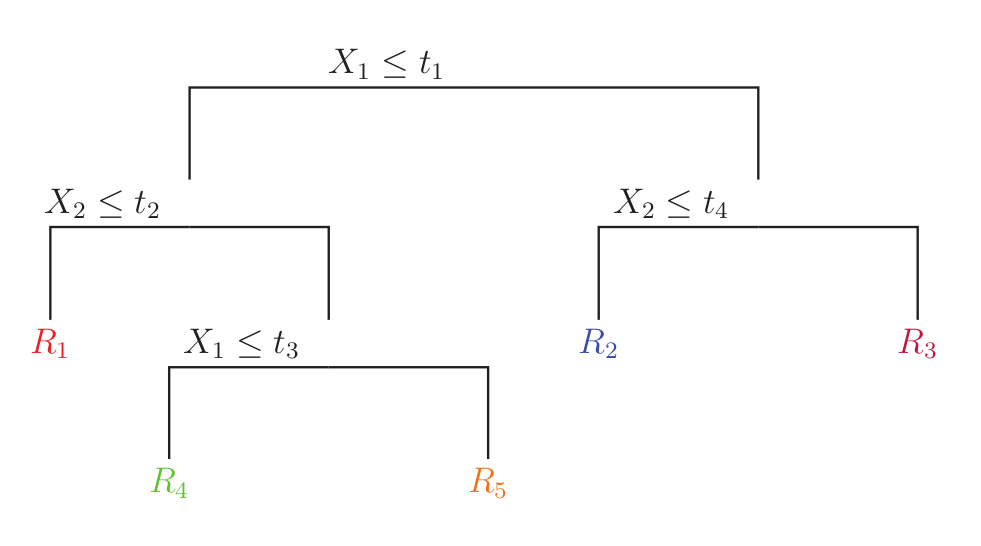
\includegraphics[width=\textwidth,height=0.3\textheight]{../fig/arvore_decisao.png}
\caption{Exemplo de árvore de decisão\label{fig:tree}}
\end{figure}

É de suma importância identificar como as árvores de regressão são
particionadas e como ocorre o seu crescimento. Os dados consistem em p
entradas e uma resposta, para cada uma das N observações: ou seja,
(\(x_i,y_i\)) para i = 1, 2, \(\dots\), N, com \(x_i\) =
(\(x_{i,1}, x_{i,2}, \dots, x_{i,p}\)). De forma automática, o algoritmo
determina as variáveis a serem utilizadas e seus pontos de divisão, além
da forma que a árvore tomará. Suponha primeiro que temos M regiões,
sendo elas \(R_1\), \(R_2\), \(\dots\), \(R_M\) e modelamos a resposta
como um \(w_m\) constante em cada região, sendo sua função estimada
escrita da seguinte maneira:

\[
\hat{f}(x) = \sum^M_{m=1}w_m I(x \in R_m),
\]

\noindent onde \(I(x \in R_m)\) denota a função indicadora para o evento
\({x \in R_m}\)

Ao adotarmos como critério a minimização da soma dos quadrados
\(\sum (y_i - f(x_i))^2\), o melhor \(w_m\) será apenas a média de
\(y_i\) na região \(R_m\):

\[\hat{w}_m= \hbox{média} (y_i|x_i \in R_m).\]

Não existe uma forma fechada (determinística) para encontrar a melhor
partição binária que minimize a soma dos quadrados dos resíduos. Por
isso, é necessário um algoritmo computacionalmente intenso, onde são
testadas diversas partições. Começando com todos os dados, considere uma
variável de divisão \(X_j\) e pontos de divisão t e a definição do par
em semiplanos.

Para variáveis numéricas, o ponto de divisão t é um valor numérico,
então tem-se:

\[R_1(j,t) = \left\{ X|X_j \leq t \right\} \hbox{ e }  R_2(j,t) = \left\{X|X_j > t \right\}\]

Para variáveis categóricas, t é um conjunto de categorias e por isso
tem-se:

\[R_1(j,t) = \left\{ X|X_j \in t \right\} \hbox{ e }  R_2(j,t) = \left\{X|X_j \notin t \right\}\]

Em seguida, busca-se a variável de divisão \(X_j\) e os pontos de
divisão t que resolvem:

\[\hat{i}(j,t) = \underset{j,t}{\min} \left[ \underset{w_1}{\min} \sum_{x_i \in R_1 (j,t)} (y_i - w_1)^2 + \underset{w_2}{\min}  \sum_{x_i \in R_2 (j,t)} (y_i - w_2)^2   \right]\]

Para qualquer opção j e t, a minimização é resolvida por:

\[\hat{w}_1 = \hbox{média}(y_i|x_i \in R_1(j,t)) \hbox{ e } \hat{w}_2 = \hbox{média} (y_i|x_i \in R_2(j,t)).\]

Tendo encontrado a melhor divisão, os dados são particionados nas duas
regiões resultantes e o processo de divisão é refeito. Então esse
processo é repetido em todas as regiões resultantes.

Para evitar o ajuste excessivo, podemos parar de cultivar a árvore se a
redução no erro não for suficiente para justificar a complexidade extra
de adicionar uma subárvore a mais. No entanto, isso pode não ser claro.
A abordagem padrão é, portanto, cultivar uma árvore ``cheia'' e depois
realizar a poda. Isso pode ser feito usando um esquema que remove as
ramificações, dando o mínimo de aumento no erro. Mais detalhes podem ser
encontrados em Breiman (\protect\hyperlink{ref-breiman1984j}{1984}).

Os principais hiperparâmetros do método são:

\begin{itemize}
\item
  Profundidade máxima e quantidade máxima de nós (altos valores podem
  apresentar problemas de \emph{overfitting});
\item
  Número mínimo de observações no nó.
\end{itemize}

As variáveis explicativas raramente são igualmente relevantes para a
previsão e criação da árvore. Frequentemente, apenas algumas delas têm
influência substancial na resposta. A grande maioria é irrelevante e
poderia muito bem não ter sido incluída. Para uma decisão simples de uma
árvore, Breiman (\protect\hyperlink{ref-breiman1984j}{1984}) propôs o
seguinte cálculo para a importância das variáveis:

\[
\Upsilon(X_j, T)= \sum_{n=1}^{J-1} \hat{i}_n(j,t) I(X_j=\iota_n),
\]

\noindent onde \(\Upsilon(X_j, T)\) é uma medida de relevância para cada
variável preditora \(X_j\) referente a árvore \(T\), \(\iota_n\) é a
variável utilizada para realizar a partição das regiões do nó \(n\),
\(\hat{i}(j, t)\) é a minimização realizada para seleção do ponto de
divisão no nó \(n\), com isso, é realizada a soma em todos os nós
internos para os quais foi escolhido como a variável de divisão.

As árvores de decisão estão na base de muitos algoritmos modernos e de
ponta, incluindo o Random Forest, ao qual utilizaremos neste trabalho.

\hypertarget{floresta-aleatuxf3ria}{%
\subsubsection{Floresta aleatória}\label{floresta-aleatuxf3ria}}

Segundo Breiman (\protect\hyperlink{ref-breiman2001random}{2001}), o
método de Florestas Aleatórias (Random Forest) consiste em criar B
árvores distintas (obtidas de B amostras bootstraps da amostra original)
e combinar seus resultados para melhorar o poder preditivo. É um
algoritmo de Machine Learning amplamente utilizado, que tem os
algoritmos \emph{bagging} e \emph{CART} como base. Porém, o problema de
utilizar o método bootstrap para a aplicação das árvores de decisão é
que possivelmente serão escolhidas as mesmas variáveis e as previsões
acabariam altamente correlacionadas (Murphy,
\protect\hyperlink{ref-murphy2012probabilistic}{2012}). Por isso, além
da reamostragem de observações, também é realizado a amostragem
aleatória de variáveis no crescimento de cada árvore. A função de
previsão pode ser escrita da seguinte maneira:

\[
\hat{f}_{RF}(x) = \frac{1}{B}\sum_{b=1}^BT_b(x)
\]

\noindent onde \(T_b\) é a estimativa da função da b-ésima árvore.

Um dos pontos negativos das árvores de decisão é que são algoritmos
instáveis, isto é, mudando um pouco os dados, a árvore criada poderá
sofrer grandes mudanças. Por isso são modelos de baixa tendência, porém
de alta variabilidade. A técnica de bootstrap tenta melhorar esse ponto
do modelo, replicando-o em diversas bases diferentes para reduzir a
variabilidade.

Neste algoritmo tem-se os hiperparâmetros herdados do modelo de árvore
de decisão e a adição de mais alguns. Os principais são:

\begin{itemize}
\item
  Quantidade de árvores que serão utilizadas. Por padrão são utilizadas
  500 árvores;
\item
  Quantidade de variáveis que serão amostradas. Por padrão são
  amostradas \(\sqrt{p}\) variáveis, onde \(p\) é a quantidade de
  variáveis totais da base;
\item
  Proporção de reamostragem das observações. Por padrão é reamostrada
  uma base do mesmo tamanho, via amostragem aleatória com reposição.
\end{itemize}

Os valores padrões descrito acima são os definidos pelo pacote Ranger
(Wright, \protect\hyperlink{ref-wright2015ranger}{2015}).

O algoritmo é descrito abaixo:

\begin{algorithm}[H]
    \Para{b \leftarrow 1 \textbf{ at\'{e} } B}{
        (1) Reamostre a base de treino via bootstrap;

        \nosemic (2) Cresça a árvore de decisão $T_b$ nesta base até atingir a profundidade máxima ou que o nó contenha o valor mínimo de observações;

        \pushline    (i) Selecionar m variáveis das p variáveis da base;

          (ii) Selecionar a variável que minimize os erros;

         (iii) Criar um nó utilizando o melhor ponto de divisão;
  }
  \Return{Ensemble das árvores \{T_e\}}

\caption{Random Forest}

\end{algorithm}

O Erro Fora da Amostra (ou \emph{out-of-bag}(OOB)) é uma das
características do próprio algoritmo, visto que, as observações são
reamostradas em cada treinamento de cada árvore. Então é possível
utilizar as observações não utilizadas na criação da árvore como teste.
Como as árvores utilizadas neste trabalho são árvores regressoras, o
erro utilizado é o Erro Quadrático Médio (EQM).

Árvores de decisão são facilmente interpretadas e podem ser visualizadas
em forma de árvores como na Figura \ref{fig:tree}, porém, quando se tem
um conjunto dessas árvores perdemos essa representação em forma de
árvore. Com isso, é necessário utilizar o cálculo de relevância que foi
comentado anteriormente, onde a relevância das variáveis em uma única
árvore de decisão (T) é representada por \(\Upsilon(X_j, T)\), por se
tratar de um conjunto de B árvores. Essa medida é facilmente expandida
para o caso de múltiplas árvores como uma média da importância para cada
árvore:

\[
\Upsilon(X_j, T_e) = \frac{1}{B} \sum^{B}_{b=1}\Upsilon(X_j, T_b). 
\]

\hypertarget{aprendizado-nuxe3o-supervisionado}{%
\section{Aprendizado Não
Supervisionado}\label{aprendizado-nuxe3o-supervisionado}}

Diferente do aprendizado supervisionado, como os três algoritmos/modelos
apresentados anteriormente, o aprendizado não supervisionado não possui
variável resposta. Neste trabalho será abordado o método K-means, que é
utilizado em tarefas de clusterização, onde o objetivo é criar uma
quantidade \(K\) de clusters utilizando os dados provenientes do site
Data.RIO (\protect\hyperlink{ref-datario}{2020}), para verificar se há
alguma relação da distribuição de propriedades e preço com variáveis
relacionadas a economia, educação e saúde do bairro.

\hypertarget{k-means}{%
\subsection{K-means}\label{k-means}}

O algoritmo de clusterização K-means (também chamado de K-médias) é
comumente usado devido a sua facilidade de implementação (Jain,
\protect\hyperlink{ref-jain1999data}{1999}). Utiliza o conceito de
centróides como padrões representativos dos grupos, onde o centróide
representa o centro de um grupo, sendo calculado pela média de todos os
objetos do grupo (Fontana, \protect\hyperlink{ref-fontanaestudo}{2009}).

De acordo com Fontana (\protect\hyperlink{ref-fontanaestudo}{2009}), o
algoritmo pode ser descrito a partir dos seguintes passos:

\begin{enumerate}
\def\labelenumi{\arabic{enumi}.}
\item
  Atribuem-se valores iniciais para os centróides seguindo algum
  critério, por exemplo, sorteio aleatório desses valores dentro dos
  limites de domínio de cada atributo;
\item
  Aloca-se para cada objeto ao grupo cujo centróides possua maior
  similaridade com o objeto;
\item
  Recalcula-se o valor do centróide de cada grupo, como sendo a média
  dos objetos atuais do grupo;
\item
  Repete-se os passos 2 e 3 até que os grupos se estabilizem.
\end{enumerate}

Na Figura \ref{fig:passo1} tem-se a execução do passo 1 e 2 do
algoritmo, a inicialização dos protótipos para atribuir cada objeto ao
grupo cujo centróides possui maior similaridade ao objeto.

\begin{figure}
\centering
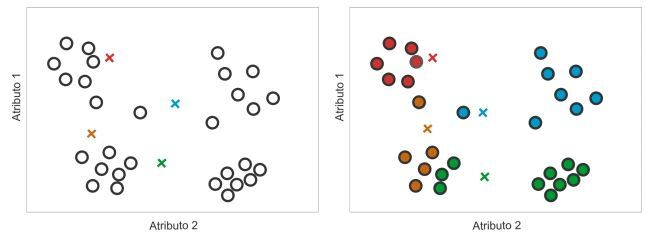
\includegraphics{../fig/passo1.jpeg}
\caption{Execução do algoritmo K-means (Parte 1).\label{fig:passo1}}
\end{figure}

Na Figura \ref{fig:passo2} tem-se a execução do passo 3, o recálculo dos
valores dos protótipos, como sendo a média dos atributos dos objetos
atualmente presentes em cada grupo para posteriormente repetir os passos
2 e 3, com a independência dos objetos dos grupos a que pertenciam.

\begin{figure}
\centering
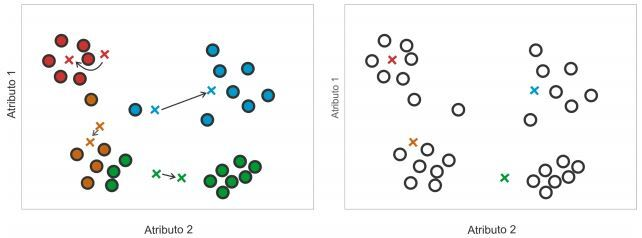
\includegraphics{../fig/passo2.jpeg}
\caption{Execução do algoritmo K-means (Parte 2).\label{fig:passo2}}
\end{figure}

Por fim, na Figura \ref{fig:passo3}, a repetição dos passos 2 e 3,
respectivamente. O algoritmo continuaria a repetir os passos 2 e 3
enquanto ocorrer alterações nos grupos.

\begin{figure}
\centering
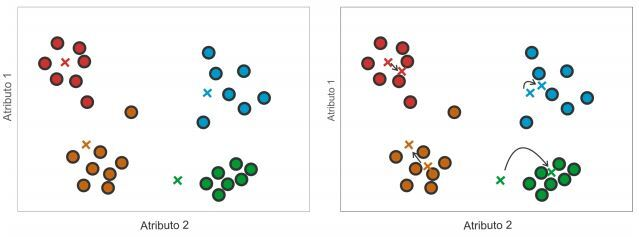
\includegraphics{../fig/passo3.jpeg}
\caption{Execução do algoritmo K-means (Parte 3).\label{fig:passo3}}
\end{figure}

Para que seja feito o processo descrito acima é necessário uma noção de
distância ou de similaridade, onde a medida mais simples, e que será
considerada neste trabalho, é a distância euclidiana entre dois pontos,
definida abaixo:

\[
d(p_1,p_2) = \sqrt{(p_1 - p_2)^2},
\]

\noindent onde \(p_1\) e \(p_1\) são dois pontos unidimensionais.

O objetivo deste algoritmo é minimizar a variabilidade dentro de cada
cluster, que pode ser definido como a soma quadrática das distâncias
euclidianas entre os itens e o centróide, como na fórmula abaixo, onde
\(x_i\) é uma observação e \(\mu_k\) é a média do cluster:

\[
W(C_k) = \sum_{x_i \in C_k}(x_i-\mu_k)^2 
\]

Para a definição da quantidade \(K\) de clusters, utiliza-se um dos
métodos mais simples conhecido como \emph{Elbow Method} (método
cotovelo), que consiste em testar quantidades de clusters até encontrar
a quantidade \(K\) onde o acréscimo de clusters não apresente uma queda
significativa na variação total dentro do cluster (WSS). Este método
inicia com apenas um cluster, armazena a variação total dentro do
cluster e incrementa a quantidade de cluster até chegar ao valor máxima
definido inicialmente. Sendo assim, quando não houver um salto relevante
entre uma quantidade de cluster e a próxima quantidade, entende-se que o
algoritmo é relevante com aquela quantidade \(K\) e então ele deve ser
usado pra segmentar os dados. A variação é representada matematicamente
abaixo:

\[
WSS = \sum_{k=1}^K W(C_k)
\]

\hypertarget{resultados}{%
\chapter{Resultados}\label{resultados}}

Este capítulo apresenta os resultados das análises descritivas dos
valores das propriedades e também um detalhamento sobre as propriedades
dispostas geograficamente. Além disso, é também retratado neste capítulo
os modelos ajustados através do método de Regressão Múltipla e Random
Forest para previsão do valor da diária, juntamente com a análise de
diagnóstico da qualidade do ajuste obtido.

\hypertarget{anuxe1lise-descritiva}{%
\section{Análise Descritiva}\label{anuxe1lise-descritiva}}

Com o objetivo de compreender melhor os fenômenos que impactam nos
preços das diárias, foi realizada a análise exploratória. A base
principal de aluguéis possui 35.793 observações de 106 variáveis. Após a
remoção de variáveis que não são relevantes para o objetivo do estudo ou
que não possuem variabilidade, além da retirada de observações com
valores faltantes na variável resposta (apenas 7 observações), passamos
a contar com 38 variáveis, sendo 9 delas criadas que serão comentadas
neste capítulo. O detalhamento desses campos se encontra no apêndice na
Tabela \ref{tab:desc_variaveis}.

Pelas estatísticas descritivas da variável preço na Tabela
\ref{tab:preco_com_outlier} é possível notar uma forte assimetria nos
dados. Além disso, é possível notar valores exorbitantes, e por isso,
serão removidos alugueis que estejam acima do limite superior (LS =
Quantil 75\% + 1.5(Quantil 75\% - Quantil 25\%)).

\begin{table}

\caption{\label{tab:preco_com_outlier}Distribuição da variável preço}
\centering
\begin{tabular}[t]{r|r|r|r|r|r}
\hline
Quantil 25\% & Quantil 50\% & Quantil 75\% & Média & Máximo & Limite Superior\\
\hline
R\$     159,00 & R\$     299,00 & R\$     649,00 & R\$     795,62 & R\$ 138.288,00 & R\$   1.384,00\\
\hline
\multicolumn{6}{l}{\textit{Fonte: } O próprio autor}\\
\end{tabular}
\end{table}

Para avaliar a distribuição da variável resposta (preço da diária),
utilizou-se um histograma e um gráfico conhecido como QQplot, onde são
comparados os quantis da variável com os quantis teóricos de uma
distribuição, que neste caso será a distribuição normal, por se tratar
de uma distribuição simétrica, além da haver a suposição de normalidade
dos erros, uma combinação linear da variável resposta. Com auxilio da
Figura \ref{dist_preco}, mesmo removendo as propriedades acima do limite
superior, ainda é possível notar uma assimetria. Como em todas as
variáveis relacionadas a preço, é comum que possua uma grande quantidade
de valores pequenos e poucos casos com valores elevados. Medidas como
correlação e média podem ser bastante influenciadas por valores extremos
e outliers. Para contornar essa influencia foi utilizada a transformação
de Box-Cox para que a distribuição da variável em análise seja simétrica
e por consequência mais próxima da distribuição normal, onde o valor de
\(\lambda\) ótimo encontrado foi -0.020202.

\begin{figure}
\centering
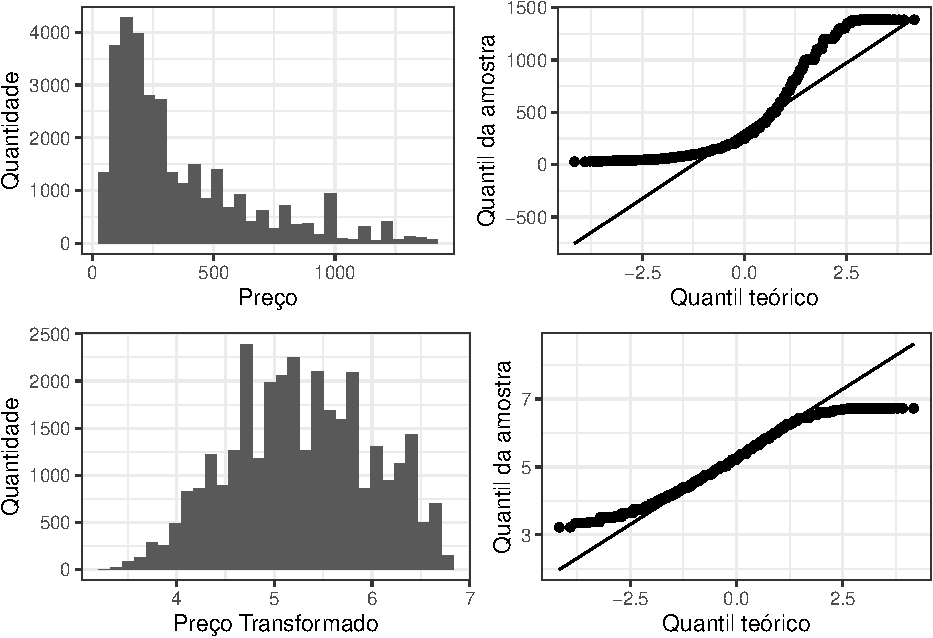
\includegraphics{00-TCC_files/figure-latex/dist_preco-1.pdf}
\caption{\label{dist_preco}Distribuição dos preços}
\end{figure}

Com os dados extraídos do site Data Rio, foi utilizado o algoritmo
k-means para separar os bairros de acordo com a similaridade entre eles.
Com base na variação total dentro do cluster e utilizando o método
``cotovelo'', foi definida a utilização de 4 clusters, pois a partir do
quinto, o ganho de performance é relativamente pequeno como pode ser
visto na Figura \ref{wss}. Verificou-se que bairros com melhores índices
relacionados a educação e economia estão no primeiro cluster, declinando
até o quarto. A média de cada variável por cluster se encontra na Tabela
\ref{tab:descritiva_cluster}. A lista detalhada dos bairros por clusters
se encontra no apêndice na Tabela \ref{tab:cluster_bairros}, mas para
uma melhor representação, podemos verifica-los geograficamente na Figura
\ref{clusters_bairros}.

\begin{figure}
\centering
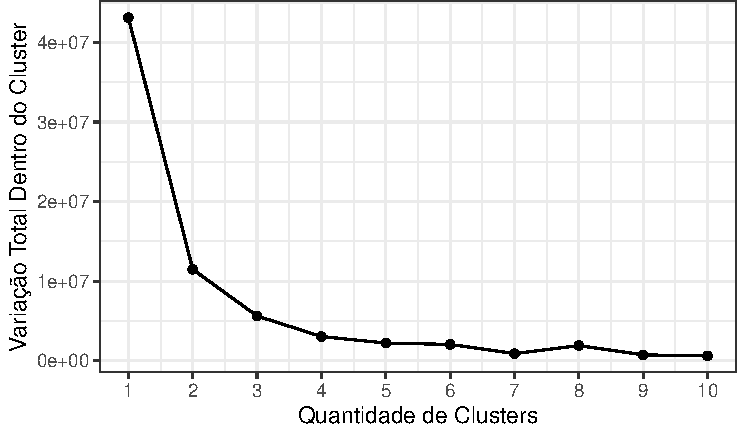
\includegraphics{00-TCC_files/figure-latex/wss-1.pdf}
\caption{\label{wss}Variação total dentro do cluster}
\end{figure}

\begin{table}

\caption{\label{tab:descritiva_cluster}Descritiva dos clusters}
\centering
\begin{tabular}[t]{l|r|r|r|r}
\hline
Variável & Cluster 1 & Cluster 2 & Cluster 3 & Cluster 4\\
\hline
IDH Longevidade & 0,89 & 0,86 & 0,81 & 0,74\\
\hline
IDH & 0,96 & 0,93 & 0,87 & 0,79\\
\hline
IDH Educação & 0,99 & 0,98 & 0,96 & 0,90\\
\hline
IDH Renda & 1,00 & 0,97 & 0,84 & 0,72\\
\hline
Esperança de Vida & 78,58 & 76,32 & 73,70 & 69,27\\
\hline
Taxa de Alfabetização Adulta & 98,97 & 97,82 & 96,98 & 94,48\\
\hline
Taxa de Frequência Escolar & 110,23 & 106,69 & 94,66 & 82,42\\
\hline
Renda per Capita & 2.418,75 & 1.346,02 & 597,95 & 309,33\\
\hline
\multicolumn{5}{l}{\textit{Fonte: } O próprio autor}\\
\end{tabular}
\end{table}

O primeiro cluster é constituído pelos bairros que apresentam os
melhores índices socioeconômicos são, também, os principais pontos
turísticos que consistem em regiões próximas de praias. São eles: Gávea,
Ipanema, Jardim Botânico, Lagoa, Leblon, Barra da Tijuca e Joá. No
cluster 2 estão os bairros de Botafogo, Copacabana, Flamengo, Glória,
Humaitá, Laranjeiras, Leme, São Conrado, Urca, Vidigal, Grumari, Recreio
dos Bandeirantes, Alto da Boa Vista, Grajaú, Maracanã, Tijuca, Méier,
Jardim Guanabara. Bairros também próximos da praia e com características
parecidas com o primeiro cluster, o bairro Vidigal, apesar de ser uma
favela, é uma área de turismo e vem entrando no roteiro principal de
quem quer fazer um tour pela cidade do Rio de Janeiro, por conter uma
das vistas mais bonitas da cidade, valorizando o bairro.
\footnote{\url{https://www.dicasdeviagem.com/morro-do-vidigal-nova-paixao-turistica-do-rio-de-janeiro/}}
No cluster 3 estão bairros próximos do centro da cidade. O quarto
apresenta bairros mais afastados das áreas turísticas e com relação aos
índices socioeconômicos, são menos qualificados.

\begin{figure}
\centering
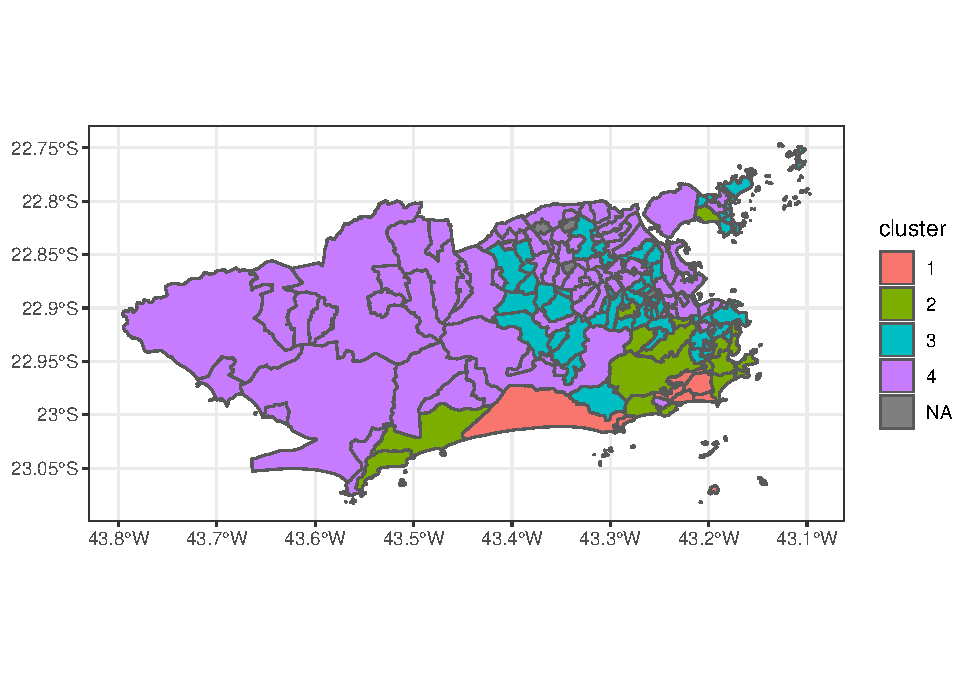
\includegraphics{00-TCC_files/figure-latex/clusters_bairros-1.pdf}
\caption{\label{clusters_bairros}Clusters dos bairros do Rio de Janeiro}
\end{figure}

Há uma maior distribuição da quantidade de locações pelas zonas sul e
central, com um maior preço mediano também (Figura
\ref{dist_preco_espaco}). Podemos notar pela Figura
\ref{boxplot_cluster} que a distribuição dos preços por clusters, de
acordo com o boxplot, decaem com relação à ``qualificação'' de cada
cluster, exceto para o último cluster. Com uma análise mais precisa, com
auxílio da Tabela \ref{tab:resumo_cluster}, que apresenta a quantidade
de propriedades, preço mediano, preço médio e a média das variáveis
quantidade máxima de hóspedes, quantidade de banheiros, quartos e camas,
e da Tabela \ref{tab:cluster_bairros}, notou-se que se trata de um
cluster com o maior número de bairros. Além disso, por ser tratar de um
cluster menos ``qualificado'' de acordo com os índices já citados,
esperávamos que houvesse propriedades com valores menores que os demais
clusters. Porém o comportamento não foi o esperado, já que os valores de
quartis (primeiro e terceiro) e limites (inferior e superior) foram
maiores que alguns clusters mais desenvolvidos. Apesar de haver uma
grande quantidade de bairros, o quarto cluster tem o menor número de
observações (locações) na base estudada (aproximadamente 11\%), o que
pode ter influenciado por valores extremos o ``mal'' comportamento em
relação aos outros grupos. Como o quarto cluster possui uma distribuição
não esperada, será criado uma variável binária ao qual identifica os
bairros pertencentes desse grupo.

\begin{figure}
\centering
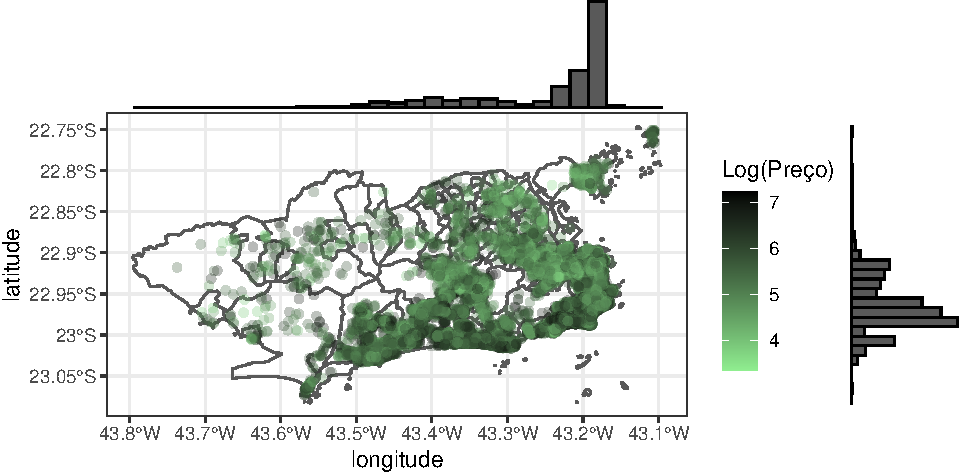
\includegraphics{00-TCC_files/figure-latex/dist_preco_espaco-1.pdf}
\caption{\label{dist_preco_espaco}Distribuição dos preços no espaço}
\end{figure}

\begin{figure}
\centering
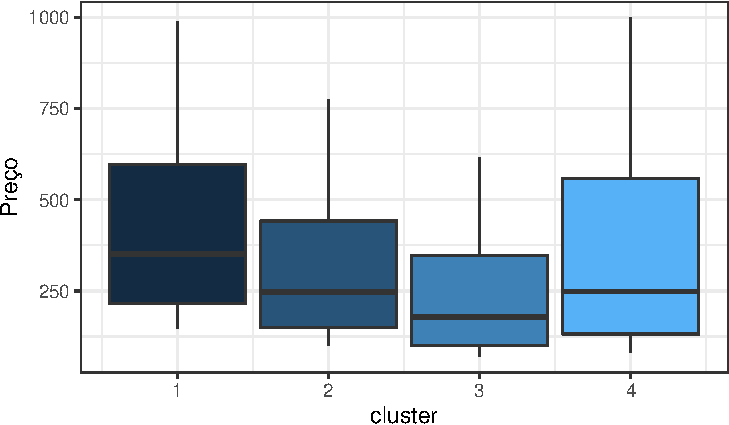
\includegraphics{00-TCC_files/figure-latex/boxplot_cluster-1.pdf}
\caption{\label{boxplot_cluster}Distribuição dos preços por cluster}
\end{figure}

\begin{table}

\caption{\label{tab:resumo_cluster}Descritiva dos clusters}
\centering
\begin{tabular}[t]{r|r|r|r|r|r|r|r}
\hline
cluster & Qtd & Preço Mediano & Preço Médio & Acomoda & Banheiros & Quartos & Camas\\
\hline
1 & 8.132 & R\$ 351,50 & R\$ 451,49 & 4,05 & 1,68 & 1,64 & 2,43\\
\hline
2 & 16.169 & R\$ 247,00 & R\$ 337,38 & 3,94 & 1,49 & 1,42 & 2,34\\
\hline
3 & 4.275 & R\$ 178,00 & R\$ 275,74 & 3,50 & 1,37 & 1,31 & 2,11\\
\hline
4 & 3.393 & R\$ 249,00 & R\$ 390,25 & 4,08 & 1,59 & 1,70 & 2,61\\
\hline
\multicolumn{8}{l}{\textit{Fonte: } O próprio autor}\\
\end{tabular}
\end{table}

Na Tabela \ref{tab:minimum_nights} são apresentados os quantis da
quantidade mínima de noites para o aluguel da propriedade. A Figura
\ref{fig:minima_noites}, no apêndice, é um exemplo de uma locação com
uma quantidade mínima de dias discrepante. A intenção é a predição de
aluguéis de propriedades a curto/médio prazo, então foram removidos os
casos onde a quantidade mínima de noites são maiores que 365 dias (um
total de 17 observações). Além disto, segundo o próprio Airbnb
(\protect\hyperlink{ref-airbnbperiodolongo}{2018}), todas as reservas de
um mês ou mais podem ser consideradas reservas de longa duração.
Criou-se, então, uma variável que identifique os aluguéis de períodos
curtos ou longos, para posteriormente verificar se há influência nos
modelos.

\begin{table}

\caption{\label{tab:minimum_nights}Quantis de quantidade mínima de dias}
\centering
\begin{tabular}[t]{l|r}
\hline
Mediana & 2\\
\hline
Quantil 99,9\% & 365\\
\hline
Máximo & 1.123\\
\hline
\multicolumn{2}{l}{\textit{Fonte: } O próprio autor}\\
\end{tabular}
\end{table}

Na central de ajuda do próprio site Airbnb
(\protect\hyperlink{ref-precoairbnb}{2020}\protect\hyperlink{ref-precoairbnb}{b})
é evidenciado que a escolha do valor da propriedade é somente do
proprietário. Contudo, a empresa sugere uma busca por espaços parecidos
com a propriedade oferecida, seja no bairro ou na cidade, para ter uma
ideia dos valores do mercado. Com isso, foram criadas variáveis de
acordo com os 15 vizinhos mais próximos dentro do mesmo cluster
utilizando a distância euclidiana, como exemplificado na Figura
\ref{vizinhos}. A escolha dos vizinhos dentro do mesmo cluster foi
realizada para não haver influência de clusters mais desenvolvidos com
clusters menos desenvolvidos ou vice-versa, o que poderia causar um viés
na estimação. Então foram criadas as seguintes variáveis: mediana do
preço dos vizinhos, quantidade mediana de quartos, camas e banheiros,
além de variáveis que identificam se a propriedade é maior (quantidade
de banheiros, quartos e camas) que a mediana dos vizinhos. A ideia
inicial era utilizar medidas estatísticas dos próprios bairros como
variáveis preditoras, como o próprio Airbnb recomenda em sua página,
porém há bairros com poucas propriedades, como pode ser visto na Tabela
\ref{tab:top_10_bairros}, o que poderia não retratar bem a realidade.

\begin{table}

\caption{\label{tab:top_10_bairros}Dez bairros com maiores medianas de preço}
\centering
\begin{tabular}[t]{l|r|r|r|r}
\hline
Bairro & Qtd & Preço Mediano & Preço Médio & Preço Máximo\\
\hline
Praia da Bandeira & 2 & R\$ 1.748,00 & R\$ 1.748,00 & R\$  3.318,00\\
\hline
Joá & 95 & R\$ 1.600,00 & R\$ 4.231,54 & R\$ 27.490,00\\
\hline
Vaz Lobo & 3 & R\$ 1.001,00 & R\$   884,33 & R\$  1.350,00\\
\hline
Engenheiro Leal & 2 & R\$   802,00 & R\$   802,00 & R\$  1.501,00\\
\hline
Ricardo de Albuquerque & 6 & R\$   776,00 & R\$   842,00 & R\$  1.999,00\\
\hline
Anchieta & 7 & R\$   703,00 & R\$ 1.350,57 & R\$  4.861,00\\
\hline
Alto da Boa Vista & 59 & R\$   698,00 & R\$ 4.204,97 & R\$138.288,00\\
\hline
Caju & 2 & R\$   660,50 & R\$   660,50 & R\$  1.199,00\\
\hline
São Conrado & 239 & R\$   500,00 & R\$ 2.265,95 & R\$ 57.180,00\\
\hline
Vicente de Carvalho & 8 & R\$   499,50 & R\$   770,75 & R\$  1.808,00\\
\hline
\multicolumn{5}{l}{\textit{Fonte: } O próprio autor}\\
\end{tabular}
\end{table}

\begin{figure}
\centering
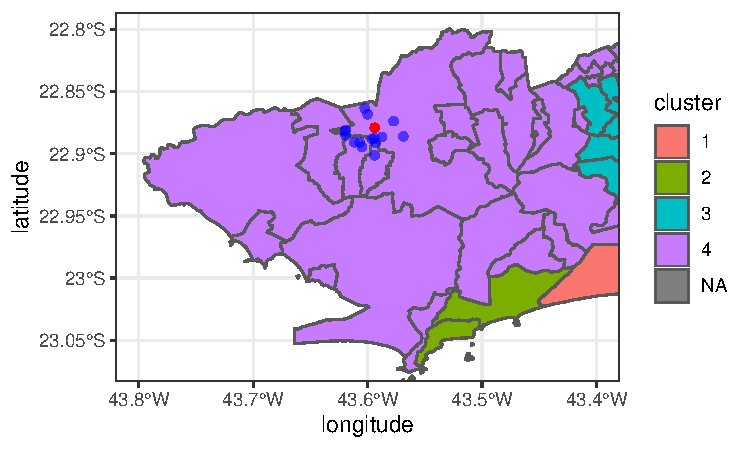
\includegraphics{00-TCC_files/figure-latex/vizinhos-1.pdf}
\caption{\label{vizinhos}Vizinhos mais próximos}
\end{figure}

\hypertarget{modelagem}{%
\section{Modelagem}\label{modelagem}}

Como temos um conjunto consideravelmente grande, para termos uma ideia
da performance dos modelos, a base de dados foi dividida em dois
pedaços: uma para treinar o modelo, com 70\% dos dados (22379
observações), e outra para teste, com os 30\% restantes (9590
observações).

\begin{figure}
\centering
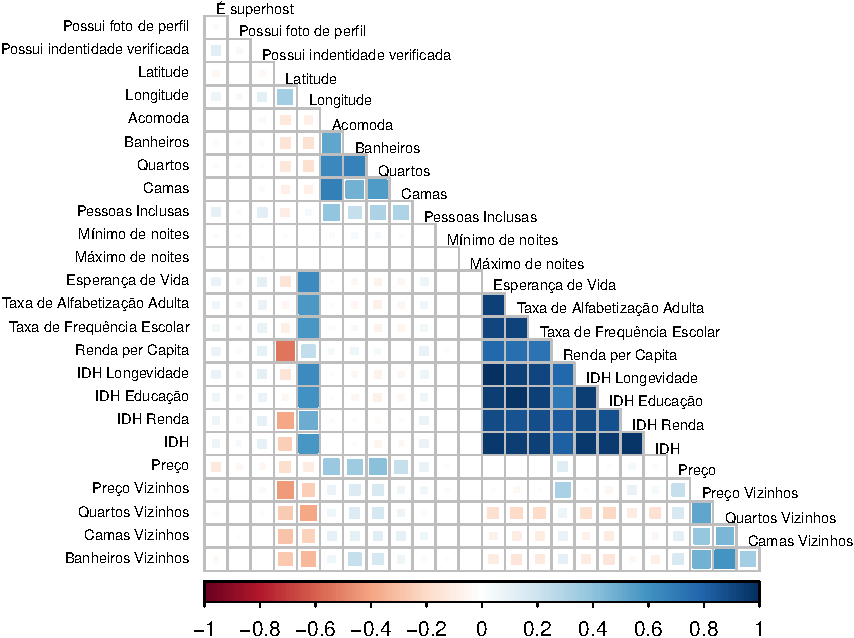
\includegraphics{00-TCC_files/figure-latex/correlacao_variaveis-1.pdf}
\caption{\label{correlacao_variaveis}Correlação entre variáveis}
\end{figure}

Ao cruzar as bases de dados utilizadas na análise, pela Figura
\ref{correlacao_variaveis} é possível notar grandes correlações entre as
variáveis da mesma base de dados (Data Rio). Comparando variáveis de
bases diferentes, há uma correlação significativa ao comparar a
\emph{Longitude} com os \emph{Índices de Desenvolvimento Humano (IDH)},
nos dando uma ideia de que há áreas que realmente são mais
desenvolvidas, o que pode ser uma variável importante para a análise.
Além disso, há uma correlação significativa e positiva do preço com as
variáveis de quantidade de quartos, banheiros e capacidade de
acomodação, nos dando uma ideia de que quanto maior a propriedade, mais
cara ela se torna.

Como a variável ``IDH'' é uma combinação de outros tipos de índices
(longevidade, educação e renda)\footnote{\url{http://www.atlasbrasil.org.br/2013/pt/o_atlas/idhm/}},
caracteriza-se problema de multicolinearidade. O mesmo se pode dizer com
a variável ``IDH de educação'' com as variáveis ``taxas de frequência
escolar'' e ``alfabetização adulta''. Com isso, vamos considerar apenas
as variáveis ``originais'', ou seja, variáveis sem qualquer tipo de
combinação. Além disto, foram verificadas as variáveis com o mesmo
problema utilizando o VIF (\emph{variance inflation factor}) como
método. Na Tabela \ref{tab:vif} é apresentada as variáveis com os
maiores índices de inflação.

\begin{table}

\caption{\label{tab:vif}VIF}
\centering
\begin{tabular}[t]{l|r}
\hline
Variavel & VIF\\
\hline
Taxa de Alfabetização Adulta & 23,15\\
\hline
Esperança de Vida & 16,46\\
\hline
Longitude & 14,10\\
\hline
Taxa de Frequência Escolar & 11,97\\
\hline
Renda per Capita & 7,71\\
\hline
Latitude & 5,78\\
\hline
É do Cluster 4 & 4,67\\
\hline
\multicolumn{2}{l}{\textit{Fonte: } O próprio autor}\\
\end{tabular}
\end{table}

Alguns autores, como, por exemplo, Chatterjee
(\protect\hyperlink{ref-chatterjee2006analysis}{2006}) e Petrini
(\protect\hyperlink{ref-petrini2012degree}{2012}), sugerem que, se
qualquer VIF exceder 10 (o que acontecerá se a correlação entre as
variáveis regressoras for maior que 0,90), então a multicolinearidade
causará efeitos nos coeficientes de regressão. Com isso, foram retiradas
as variáveis Taxa de Alfabetização Adulta, Esperança de Vida, Longitude
e Taxa de Frequência Escolar, pois apresentaram um fator acima da
referencia escolhida (\(VIF>10\)). Após a remoção das possíveis
variáveis com o problema de multicolinearidade, a Tabela
\ref{tab:vif_final} apresenta as variáveis de maiores VIFs, o que não
representa mais um problema.

\begin{table}

\caption{\label{tab:vif_final}VIF pós remoção}
\centering
\begin{tabular}[t]{l|r}
\hline
Variavel & VIF\\
\hline
Latitude & 3,94\\
\hline
Quartos & 3,47\\
\hline
Renda per Capita & 3,01\\
\hline
Acomoda & 2,93\\
\hline
Quartos Vizinhos & 2,65\\
\hline
Banheiros Vizinhos & 2,60\\
\hline
Camas & 2,49\\
\hline
\multicolumn{2}{l}{\textit{Fonte: } O próprio autor}\\
\end{tabular}
\end{table}

\hypertarget{modelo-baseline}{%
\subsection{Modelo baseline}\label{modelo-baseline}}

Somente para efeitos comparativos, será criado um modelo
\emph{baseline}, onde a previsão será o preço mediano dos 15 vizinhos
mais próximos, já que, como explicado, Airbnb
(\protect\hyperlink{ref-precoairbnb}{2020}\protect\hyperlink{ref-precoairbnb}{b})
sugere uma busca por espaços parecidos da propriedade oferecida na sua
cidade ou bairro, para ter uma ideia dos valores. Como a pesquisa está
sendo realizada na cidade do Rio de Janeiro, optamos por utilizar os
vizinhos próximos, desde que estejam no mesmo cluster, para não haver
uma influência de qualificação do bairro de acordo com os índices já
citados no capítulo de análise exploratória.

\hypertarget{modelos-lineares}{%
\subsection{Modelos Lineares}\label{modelos-lineares}}

Encontradas as estimativas dos coeficientes \(\beta\)'s, é necessário
validar o modelo de regressão, que consiste em verificar se as variáveis
fazem sentido no contexto do fenômeno estudado, que pode ser feito
através do teste t de Student como será apresentado na análise dos
resultados (Werkema, \protect\hyperlink{ref-werkema1996analise}{1996}).
Utilizando um nível de significância de 5\%, verifica-se pela Figura
\ref{significancia_ml} as variáveis com o p-valor acima dos 5\%. As
variáveis relacionadas aos pontos coloridos (vermelho ou azul) que,
mesmo com o p-valor acima do nível de significância escolhido, foram
mantidas, pois trata-se de categorias significativas de algumas
variáveis categóricas, influenciando na predição do valor de forma
negativa e positiva, respectivamente. Sendo assim, foi decidido que
haveria boa relevância para o modelo e, com isso, não serão removidas.

\begin{figure}
\centering
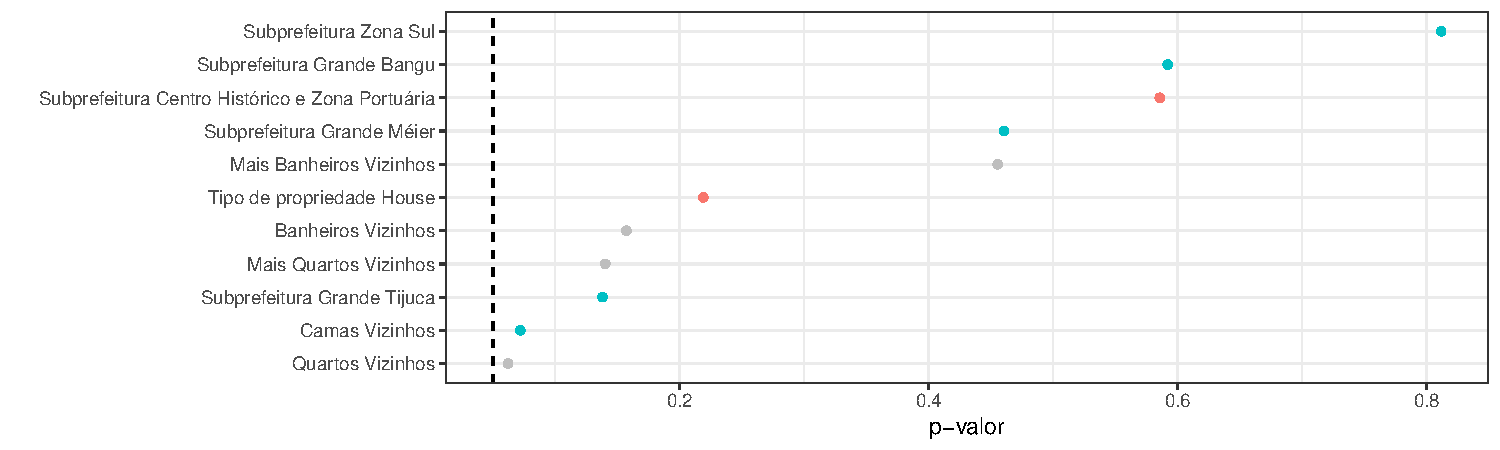
\includegraphics{00-TCC_files/figure-latex/significancia_ml-1.pdf}
\caption{\label{significancia_ml}Significância das variáveis no modelo
linear}
\end{figure}

Além da significância das variáveis comentadas anteriormente, é possível
quantificar a importância de cada variável. Para isso, será utilizado o
valor absoluto da estatística de teste utilizada para o teste de
hipóteses da significância de cada variável. Verifica-se, com isso, as
variáveis relevantes em ordem decrescente na Figura \ref{imp_ml}.

\begin{figure}
\centering
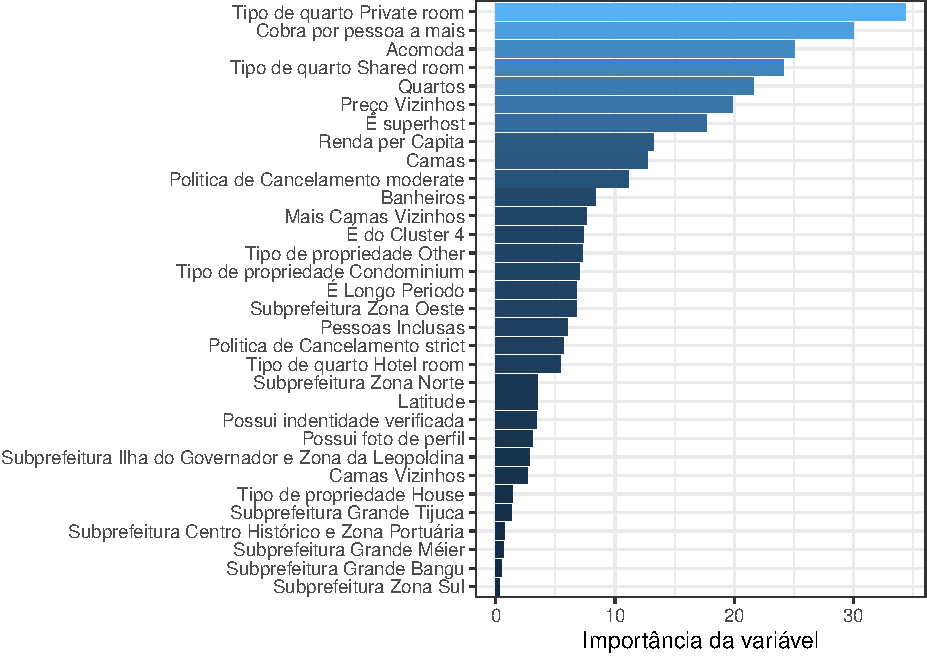
\includegraphics{00-TCC_files/figure-latex/imp_ml-1.pdf}
\caption{\label{imp_ml}Importância das variáveis no modelo linear}
\end{figure}

A adequação do modelo é realizada essencialmente por meio dos resíduos
do modelo ajustado. Após utilizar a transformação Box-Cox na variável
resposta, as Figuras \ref{resid_ml} e \ref{resid_ml_test} mostram
gráficos de adequação, com as suposições de normalidade e
homocedasticidade dos resíduos aparentemente atendidas pelos dados,
tanto na base de teste quanto na de treino.

\begin{figure}
\centering
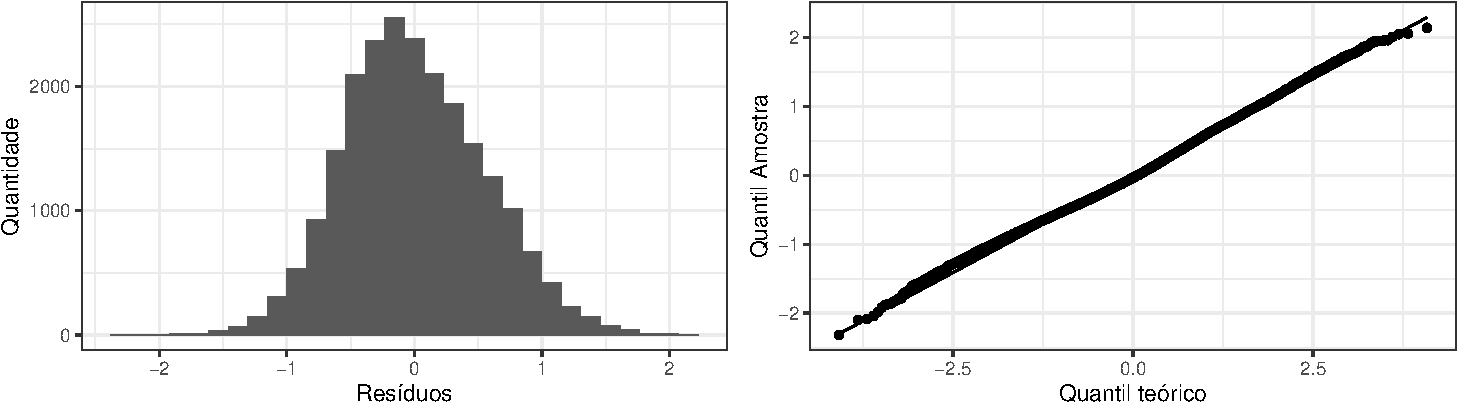
\includegraphics{00-TCC_files/figure-latex/resid_ml-1.pdf}
\caption{\label{resid_ml}Resíduos do Modelo Linear na base de treino}
\end{figure}

\begin{figure}
\centering
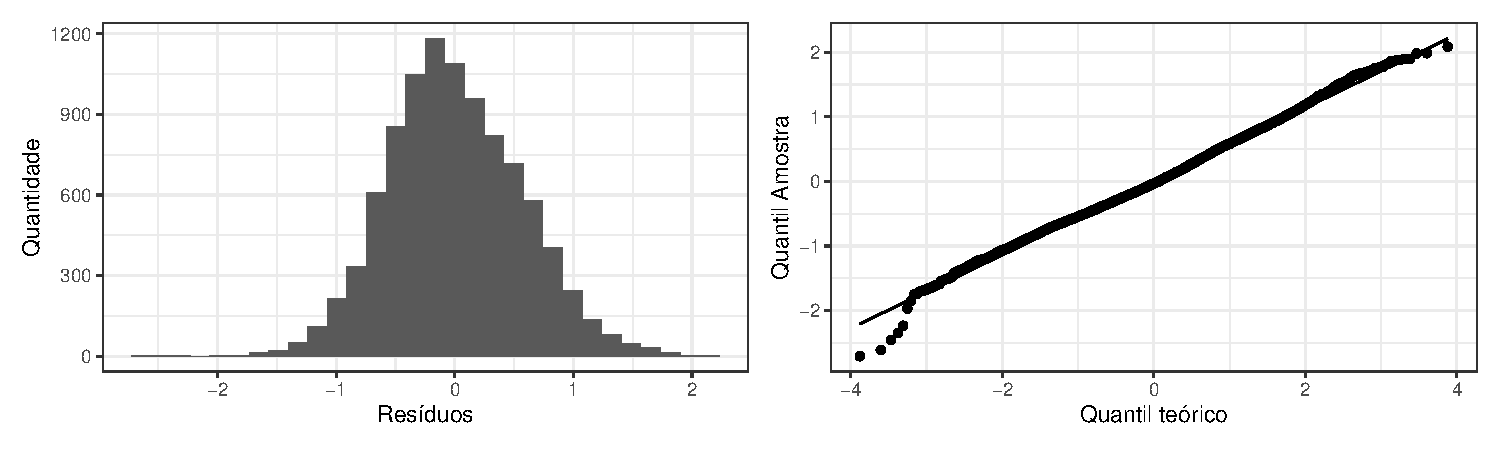
\includegraphics{00-TCC_files/figure-latex/resid_ml_test-1.pdf}
\caption{\label{resid_ml_test}Resíduos do Modelo Linear na base de
teste}
\end{figure}

Após isso, precisou verificar a previsão na escala original. Com isso,
foi aplicado uma transformação inversa na predição do preço para uma
melhor avaliação do modelo. Verifica-se, na Figura \ref{resid_ml_inv},
uma maior concentração dos resíduos em torno do zero, com uma leve
assimetria. Apesar de um grande número de previsões com baixo erro, o
modelo subestima algumas propriedades, já que os valores reais são, em
pequenas quantidades, desvalorizadas pelo modelo.

\begin{figure}
\centering
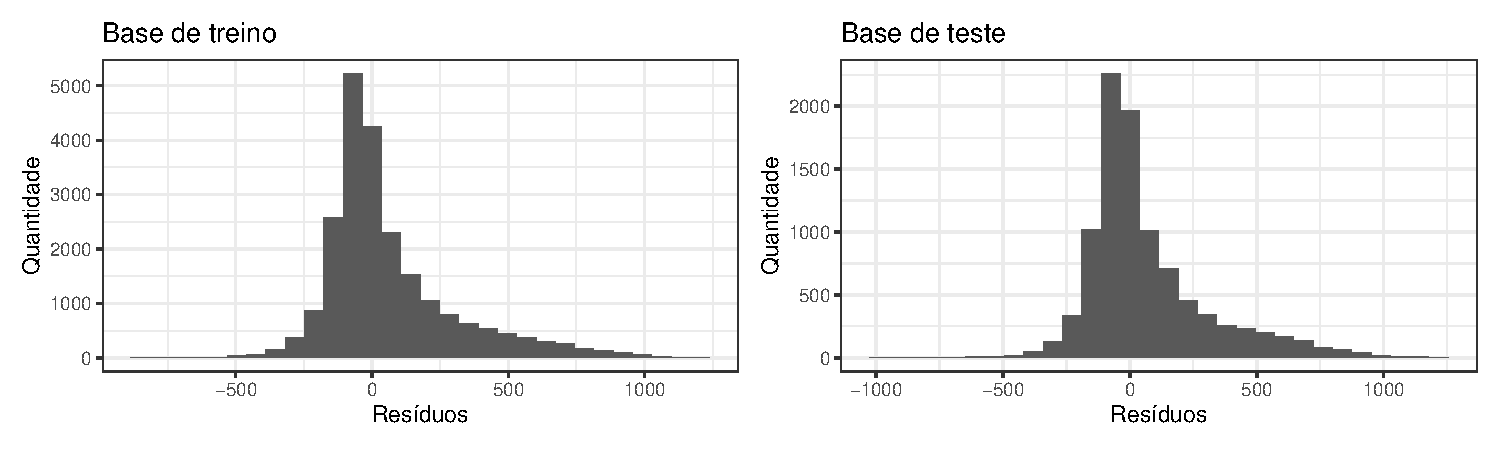
\includegraphics{00-TCC_files/figure-latex/resid_ml_inv-1.pdf}
\caption{\label{resid_ml_inv}Resíduos do Modelo Linear com Transformação
Inversa}
\end{figure}

\begin{table}

\caption{\label{tab:lm_metricas}Estimativa do erro destransformado para o Modelo Linear}
\centering
\begin{tabular}[t]{l|r|r|r|r}
\hline
Base & REQM & EAM & EPAM & R2\\
\hline
Treino & 251,93 & 166,80 & 54,23 & 0,32\\
\hline
Teste & 254,49 & 169,16 & 55,66 & 0,32\\
\hline
\multicolumn{5}{l}{\textit{Fonte: } O próprio autor}\\
\end{tabular}
\end{table}

A Figura \ref{graf_resid_ml} é dividida em dois gráficos: o gráfico
superior representa o EPAM para cada faixa de preço e a parte inferior
representa a quantidade de propriedades também pela faixa de preço. Com
isso, pode-se proferir que o método apresenta um nível não confiável
para preços baixos (\(\leq\) R\$51,00), visto que seu EPAM foi de 239,5,
ou seja, 239,5\% de erro percentual. E não há uma relação entre a
quantidade de propriedades com o EPAM, já que há grandes erros
relacionados as faixas com muitas ou poucas propriedades, como por
exemplo nas duas primeiras faixas de preço.

\begin{figure}
\centering
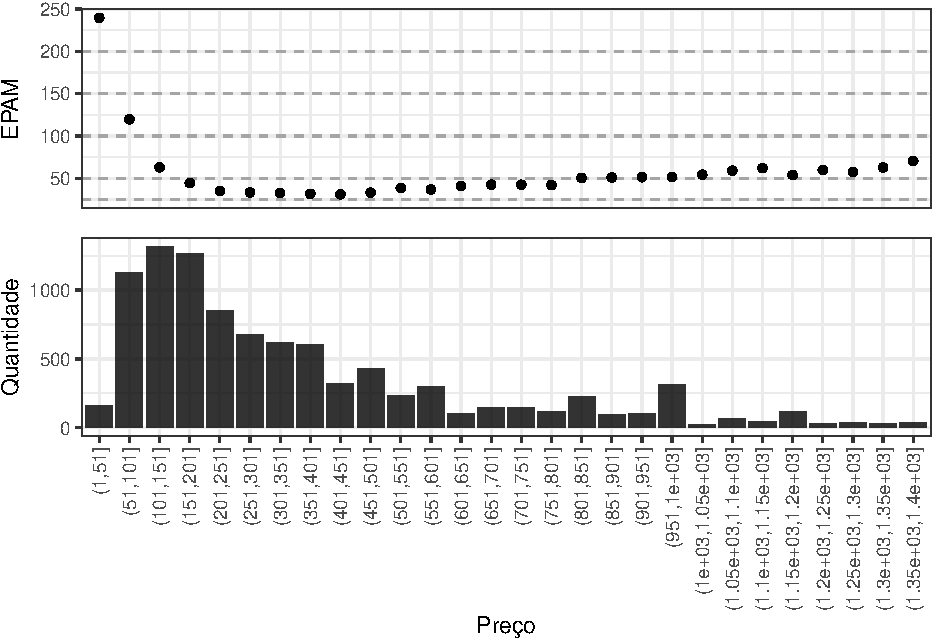
\includegraphics{00-TCC_files/figure-latex/graf_resid_ml-1.pdf}
\caption{\label{graf_resid_ml}Distribuição dos resíduos do Modelo
Linear}
\end{figure}

\hypertarget{regularizauxe7uxe3o-1}{%
\subsubsection{Regularização}\label{regularizauxe7uxe3o-1}}

Neste capítulo será testada a regularização LASSO, que é utilizada para
seleção de variáveis. Serão utilizadas as variáveis que foram removidas
(seja por significância ou multicolinearidade), de forma a compararmos a
forma de seleção utilizando este método e o método ``manual''. Um
estimador com base em apenas um subconjunto das variáveis explicativas
tem ainda mais motivos para ter uma performance boa: são comuns os
problemas em que esperamos que algumas das covariáveis não influenciem
(ou influenciem pouco) a variável resposta.

Cada valor do parâmetro \(\lambda\) leva a um conjunto de coeficientes
estimados diferentes, e o mesmo foi escolhido pela validação cruzada
neste trabalho. O mesmo pode variar entre aproximadamente 0,0002 e 0,3,
Para mais detalhes, ver Friedman
(\protect\hyperlink{ref-friedman2010regularization}{2010}).

Na Figura \ref{lasso_lambda} é apresentado o resultado da validação
cruzada e no topo da mesma é apresentada a quantidade de variáveis
selecionadas pelo algoritmo LASSO.

\begin{figure}
\centering
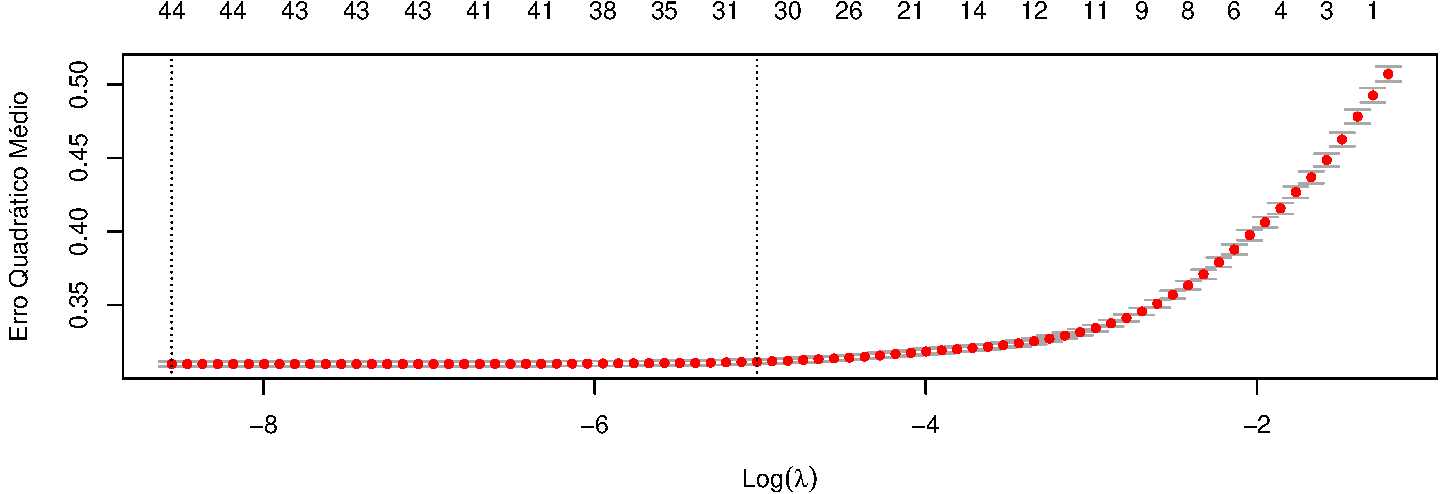
\includegraphics{00-TCC_files/figure-latex/lasso_lambda-1.pdf}
\caption{\label{lasso_lambda}Teste de valores do hiperparâmetro}
\end{figure}

Foi considerado o maior valor de \(\lambda\), de modo que o erro esteja
dentro de um erro padrão do mínimo, ou seja, será selecionado o
\(\lambda\) que apresente a quantidade mínima de variáveis de modo que o
erro médio na bases de teste (da validação cruzada) esteja dentro do
intervalo de um desvio padrão. O valor de \(\lambda\) encontrado foi
0,0066053.

Com a regressão de LASSO, os coeficientes de regressão para variáveis
sem importância são reduzidos a zero, o que efetivamente os remove do
modelo e produz um modelo mais simples que seleciona apenas os
preditores mais importantes. Conforme Figura \ref{significancia_lasso},
as variáveis removidas estão sinalizadas com pontos cinzas, enquanto os
pontos azuis e vermelhos continuam no modelo, impactando no valor da
diária de forma positiva e negativa, respectivamente.

Sem a utilização do método LASSO, foram removidas as variáveis levando
em conta problemas de multicolinearidade (IDH Educação, IDH Renda, IDH
Longevidade, IDH, Taxa de Alfabetização Adulta, Esperança de Vida,
Longitude e Taxa de Frequência Escolar) e significância (Banheiros
Vizinhos, Quartos Vizinhos, Mais Banheiros Vizinhos e Mais Quartos
Vizinhos). Com a utilização do método LASSO, foram removidas as
variáveis de acordo com a penalização do próprio método (Longitude, Tipo
de propriedade House, Mínimo de noites, Máximo de noites, Subprefeitura
Grande Bangu, Subprefeitura Grande Méier, Subprefeitura Grande Tijuca,
Subprefeitura Zona Sul, Esperança de Vida, Taxa de Alfabetização Adulta,
Taxa de Frequência Escolar, IDH Longevidade, IDH Renda, IDH, Camas
Vizinhos e Mais Banheiros Vizinhos).

Por se tratar de métodos diferentes para escolha de variáveis
regressoras, será ajustado dois modelos lineares para efeitos de
comparação: Modelo de Regressão Linear Múltipla com seleção manual das
variáveis e Modelo de Regressão Linear Múltipla com seleção das
variáveis utilizando LASSO.

\begin{figure}
\centering
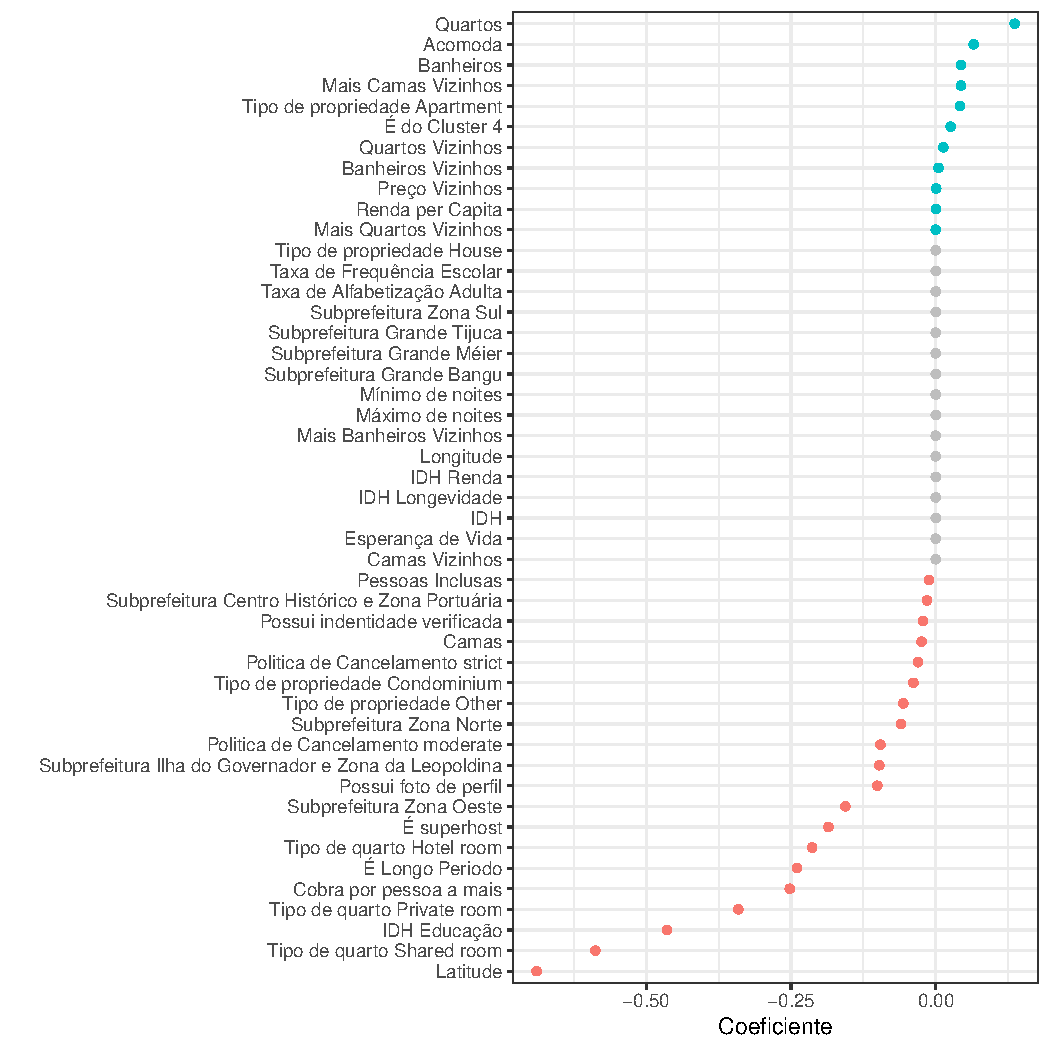
\includegraphics{00-TCC_files/figure-latex/significancia_lasso-1.pdf}
\caption{\label{significancia_lasso}Coeficientes das variáveis da
regressão Lasso}
\end{figure}

Cabe ressaltar que a seleção de variáveis via LASSO solucionou o
problema existente de multicolinearidade da base de dados, pode-se
verificar isso pela Tabela \ref{tab:vif_lasso}.

\begin{table}

\caption{\label{tab:vif_lasso}VIF Lasso}
\centering
\begin{tabular}[t]{l|r}
\hline
Variavel & VIF\\
\hline
IDH Educação & 8,56\\
\hline
Subprefeitura & 7,48\\
\hline
Renda per Capita & 5,43\\
\hline
É do Cluster 4 & 4,90\\
\hline
Latitude & 4,56\\
\hline
Quartos & 3,38\\
\hline
Acomoda & 2,93\\
\hline
\multicolumn{2}{l}{\textit{Fonte: } O próprio autor}\\
\end{tabular}
\end{table}

Assim como nos modelos lineares com a seleção de variáveis utilizando
métodos de significância e multicolinearidade, o modelo linear
utilizando LASSO também utilizou a transformação Box-Cox na variável
resposta. Conforme as Figuras \ref{resid_lasso} e
\ref{resid_lasso_test}, as suposições de normalidade e homocedasticidade
dos resíduos foram aparentemente atendidas, tanto na base de teste
quanto na de treino.

\begin{figure}
\centering
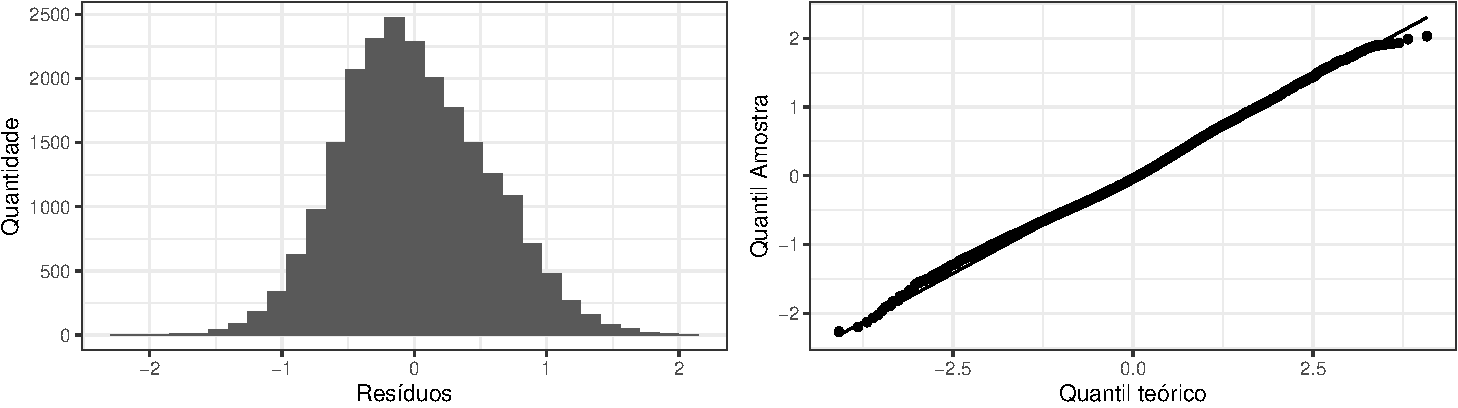
\includegraphics{00-TCC_files/figure-latex/resid_lasso-1.pdf}
\caption{\label{resid_lasso}Resíduos do Modelo Linear na base de treino}
\end{figure}

\begin{figure}
\centering
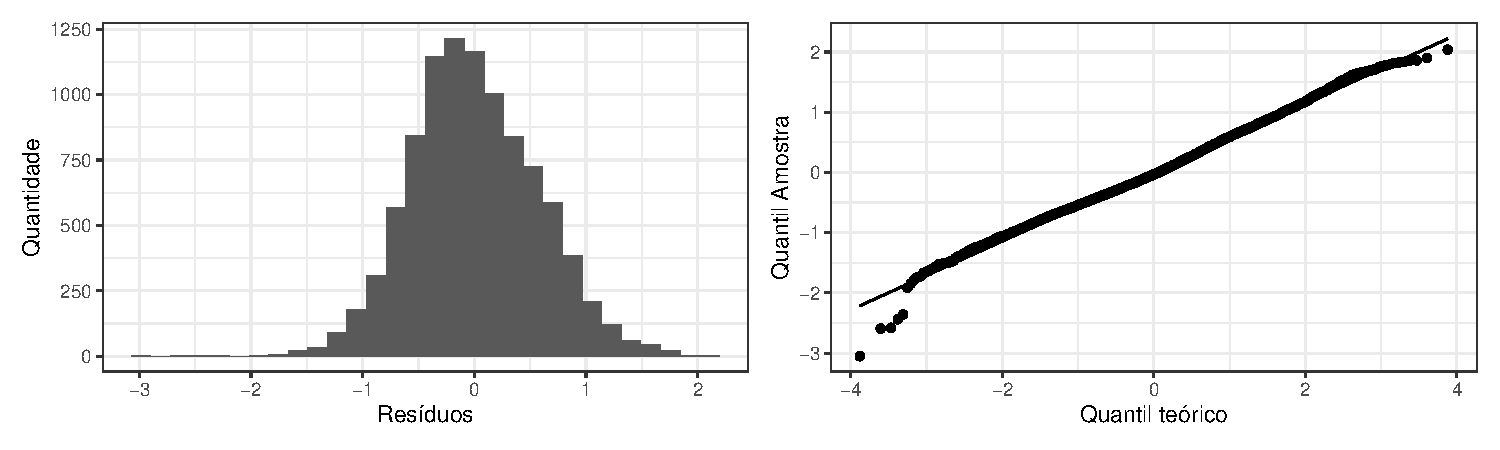
\includegraphics{00-TCC_files/figure-latex/resid_lasso_test-1.pdf}
\caption{\label{resid_lasso_test}Resíduos do Modelo Linear na base de
teste}
\end{figure}

Verificou-se também a previsão aplicando uma transformação inversa na
predição do preço para uma melhor avaliação do modelo, com auxílio da
Figura \ref{resid_lasso_inv}, verifica-se uma maior concentração dos
resíduos em torno do zero, com uma leve assimetria. Apesar de um grande
número de previsões com baixo erro, o modelo com LASSO também subestima
algumas propriedades.

\begin{figure}
\centering
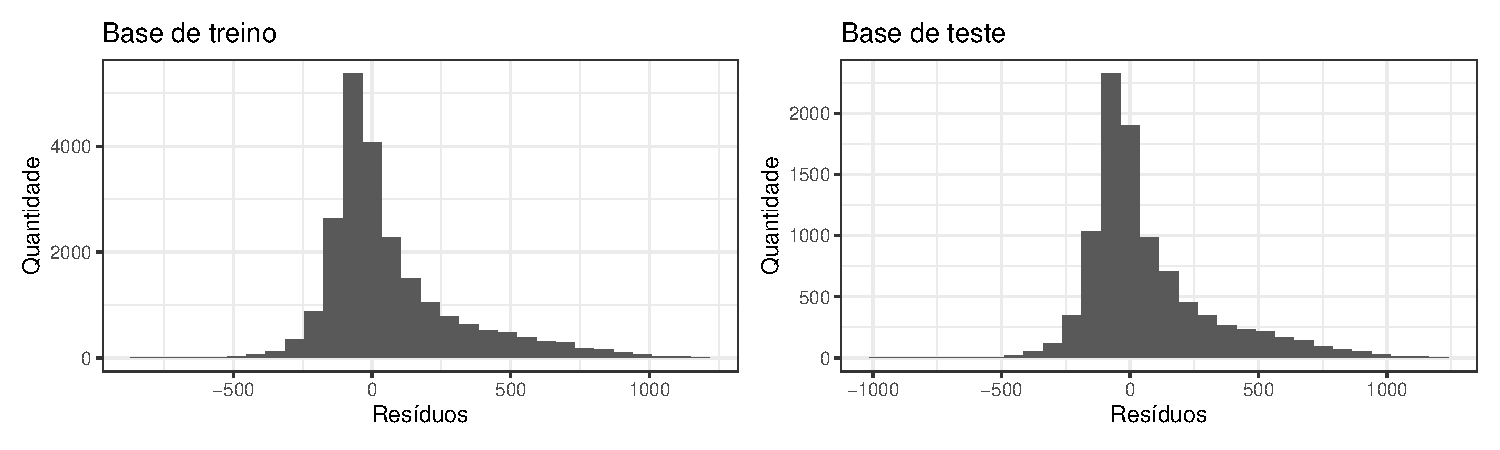
\includegraphics{00-TCC_files/figure-latex/resid_lasso_inv-1.pdf}
\caption{\label{resid_lasso_inv}Resíduos do Modelo Linear com
Transformação Inversa}
\end{figure}

\begin{table}

\caption{\label{tab:lasso_metricas}Estimativa do erro destransformado para o LASSO}
\centering
\begin{tabular}[t]{l|r|r|r|r}
\hline
Base & REQM & EAM & EPAM & R2\\
\hline
Treino & 253,79 & 167,52 & 54,46 & 0,31\\
\hline
Teste & 256,35 & 169,83 & 55,95 & 0,31\\
\hline
\multicolumn{5}{l}{\textit{Fonte: } O próprio autor}\\
\end{tabular}
\end{table}

Comparando a distribuição dos resíduos do modelos linear utilizando as
variáveis selecionadas manualmente e via LASSO pelas Figura
\ref{resid_ml_inv} e \ref{resid_lasso_inv}, é possível notar grande
semelhança. Para uma melhor comparação, também pode-se utilizar as
métricas dos erros disponíveis nas Tabelas \ref{tab:lm_metricas} e
\ref{tab:lasso_metricas}, confirmando a similaridade dos modelos
lineares.

A regressão linear utilizando LASSO se mostrou muito efetiva para
contornar problemas de multicolinearidade, (Tabela \ref{tab:vif_lasso})
e remoção de variáveis não significativas. Trata-se de um método que
torna o modelo parcimonioso sem perder tanto poder preditivo (aumento
dos erros).

\hypertarget{random-forest}{%
\subsection{Random Forest}\label{random-forest}}

\hypertarget{modelo-base}{%
\subsubsection{Modelo base}\label{modelo-base}}

Como descrito na metodologia, o modelo Random Forest possui alguns
hiperparâmetros, sendo estes definidos por valores fixos. Nesta seção,
será analisado o modelo base, ou seja, utilizando os valores dos
hiperparâmetros \emph{default} do pacote \emph{ranger} (Wright,
\protect\hyperlink{ref-wright2015ranger}{2015}).

Para efeitos de comparação, o treinamento do modelo base levou
aproximadamente 13 segundos e a predição da base de treino levou 1,28
segundos, aproximadamente.

Na Tabela \ref{tab:rf0_metricas}, é possível notar que há um ajuste em
excesso no conjunto de dados de treino (menores erros) comparado ao
conjunto de dados de teste (maiores erros), podendo por isso ter um mau
desempenho preditivo quando aplicados a novos dados, dando indícios de
sobreajuste do modelo.

\begin{table}

\caption{\label{tab:rf0_metricas}Estimativa do erro destransformado para o random forest base}
\centering
\begin{tabular}[t]{l|r|r|r|r}
\hline
Base & REQM & EAM & EPAM & R2\\
\hline
Treino & 148,54 & 87,83 & 23,98 & 0,84\\
\hline
Teste & 243,83 & 159,41 & 50,10 & 0,39\\
\hline
\multicolumn{5}{l}{\textit{Fonte: } O próprio autor}\\
\end{tabular}
\end{table}

\hypertarget{hiperparuxe2metros}{%
\subsubsection{Hiperparâmetros}\label{hiperparuxe2metros}}

Como visto na seção anterior, o modelo \emph{default} parece ter
apresentado problema de sobreajuste na base de treino. Com isso, nessa
seção abordaremos uma análise e descrição da relação entre os
hiperparâmetros do modelo, buscando valores para os mesmos, a fim de
melhorar o modelo.

Em geral, uma quantidade elevada de árvores aumenta a performance e
torna as predições mais estáveis, mas também torna a computação mais
lenta. Então é interessante encontrar um meio termo: um erro baixo com
uma quantidade de árvores não tão alta.

Como pode ser visto na Figura \ref{qtd_arvores}, o aumento na quantidade
de árvores e mantendo os demais parâmetros sem alteração, implica na
melhora (diminuição) das métricas de erro.

\begin{figure}
\centering
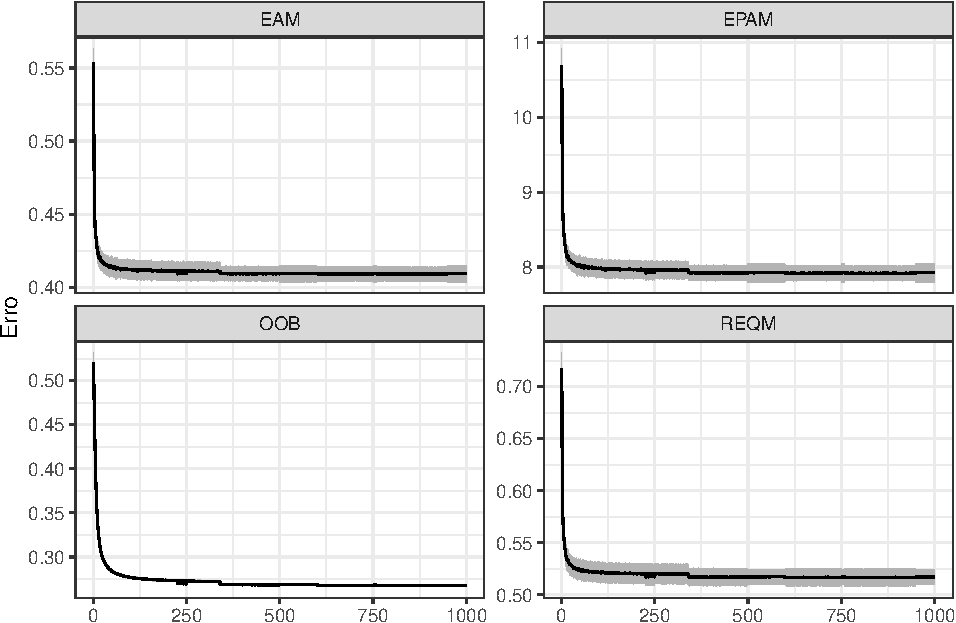
\includegraphics{00-TCC_files/figure-latex/qtd_arvores-1.pdf}
\caption{\label{qtd_arvores}Teste de quantidade de árvores}
\end{figure}

Na Figura \ref{qtd_arvores_zoom} temos o zoom a partir de 20 árvores,
para se ter um melhor discernimento de como os erros se comportam. Nesta
figura, a linha azul representa o erro da maior floresta (1000 árvores).
É possível notar que a partir de 400 árvores os erros parecem apresentar
uma certa estabilidade. Em ambas imagens, a área sombreada representa um
desvio padrão acima e abaixo da média do zero.

\begin{figure}
\centering
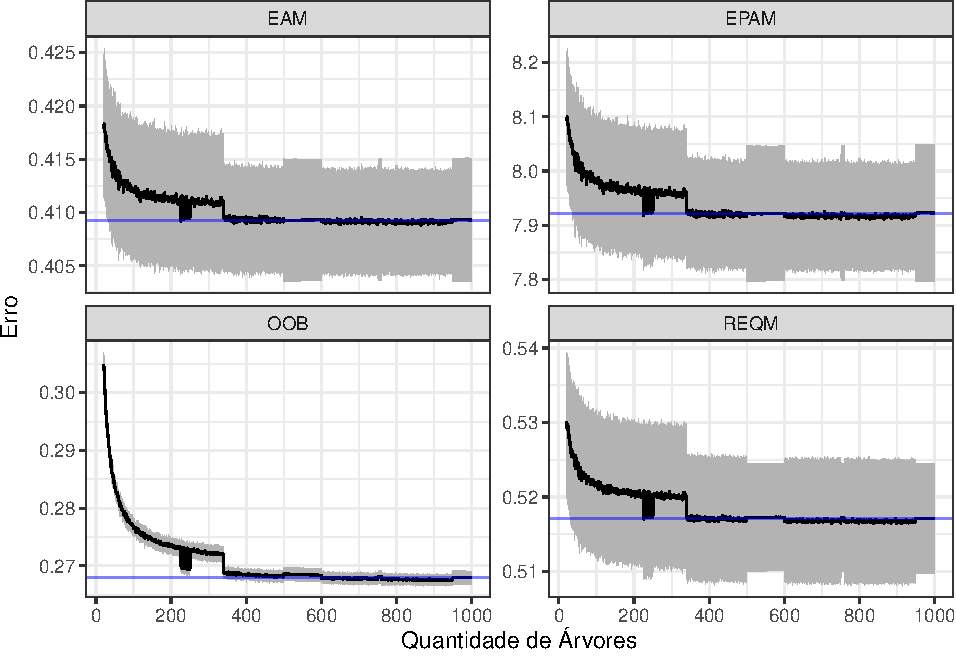
\includegraphics{00-TCC_files/figure-latex/qtd_arvores_zoom-1.pdf}
\caption{\label{qtd_arvores_zoom}Teste de quantidade de árvores - Acima
de 100 árvores}
\end{figure}

De maneira contrária, permitir árvores mais profundas ou com nós com uma
quantidade menor de observações, permite que as árvores individuais
sofram sobreajuste, que pode prejudicar o modelo final.

Não é possível realizar essa análise para os 3 hiperparâmetros
separadamente e depois unir, pois eles são altamente correlacionados
entre si. Com isso, eles precisam ser otimizados conjuntamente. Será
optado por utilizar um algoritmo para essa otimização que será abordado
no próximo tópico.

\hypertarget{otimizauxe7uxe3o}{%
\subsubsection{Otimização}\label{otimizauxe7uxe3o}}

Como comentado anteriormente é necessário realizar uma otimização dos
hiperparâmetros do modelo. Para testar tal otimização, será utilizada a
validação cruzada, onde a base de treino será separada em 10 partes.

Será definida que a quantidade de árvores poderá variar entre 1 e 2.000
árvores, a profundidade máxima poderá variar entre 0 (sem limite) e 30
nós, a quantidade de elementos mínimos no nó pode variar entre 0 (sem
limite) e 100. Considerando todos esses intervalos, temos 6.262.000
combinações possíveis de hiperparâmetros a serem testados e, por isso,
será utilizado o Algoritmo \ref{alg:hiper}, que se encontra no apêndice,
para encontrar um bom conjunto de hiperparâmetros. O algoritmo tem como
ideia principal dois pontos:

\begin{itemize}
\item
  A exploração: é realizada uma amostra aleatória de tamanho 10 do
  conjuntos de hiperparâmetros não testados;
\item
  A otimização: com o histórico dos hiperparâmetros testados e do erro
  encontrado, é treinado um modelo de Random Forest e feita a previsão
  de 10 pontos com menores erros, após isso é feita a avaliação desses
  10 pontos.
\end{itemize}

Com isso, foram testados um total de 4872 combinações de
hiperparâmetros, aproximadamente 0,08\% das possibilidades. Na Figura
\ref{otimizacao} é possível verificar a evolução do erro em cada rodada
do algoritmo, e com isso, é possível notar que a partir da rodada 60 não
há ganho na performance do modelo.

\begin{figure}
\centering
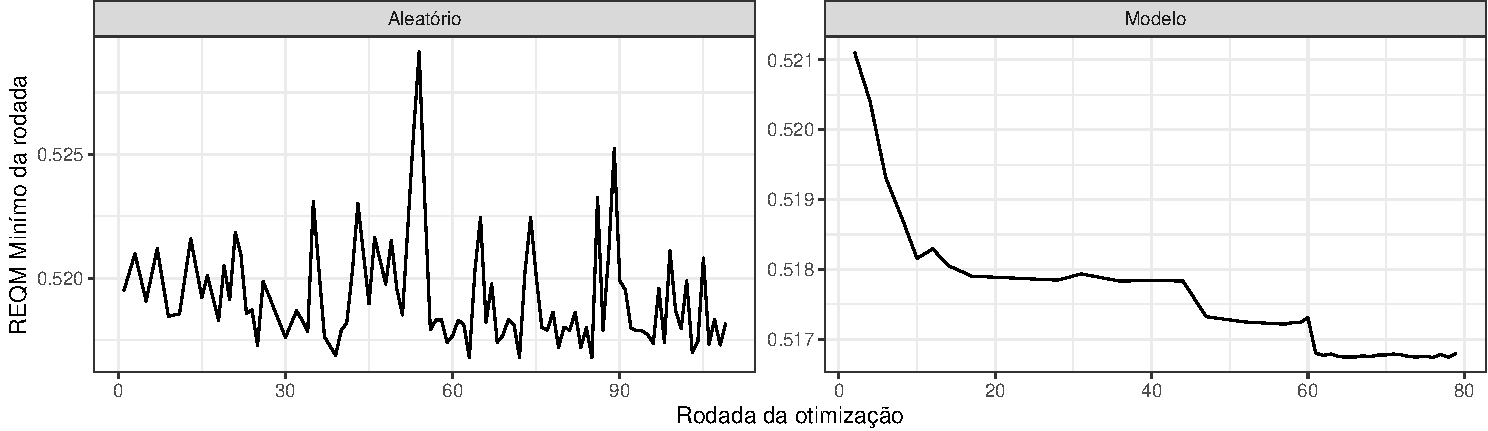
\includegraphics{00-TCC_files/figure-latex/otimizacao-1.pdf}
\caption{\label{otimizacao}Otimização dos hiperparâmetros}
\end{figure}

Com a otimização, optou-se por 50 árvores, com uma profundidade máxima
de 18 e uma quantidade mínima de 33 observações como uma quantidade
ótima de hiperparâmetros. Comparando os erros do modelo base (Tabela
\ref{tab:rf0_metricas}) com os erros do modelo otimizado (Tabela
\ref{tab:rf1_metricas}), pode-se notar que esse conjunto apresenta um
resultado bem próximo do modelo \emph{default} na base de teste, porém
sendo muito mais simples e com resultados mais próximos entre as bases
de treino e teste, que é um bom indicativo que o modelo não está com
sobreajuste.

Após o treinamento dos dados, na Figura \ref{imp_var_rf} são
apresentadas as principais variáveis na ordem decrescente de
importância. No topo, variáveis que se ``relacionam'' com o tamanho da
propriedade, como quantidade de quartos e banheiros.

\begin{figure}
\centering
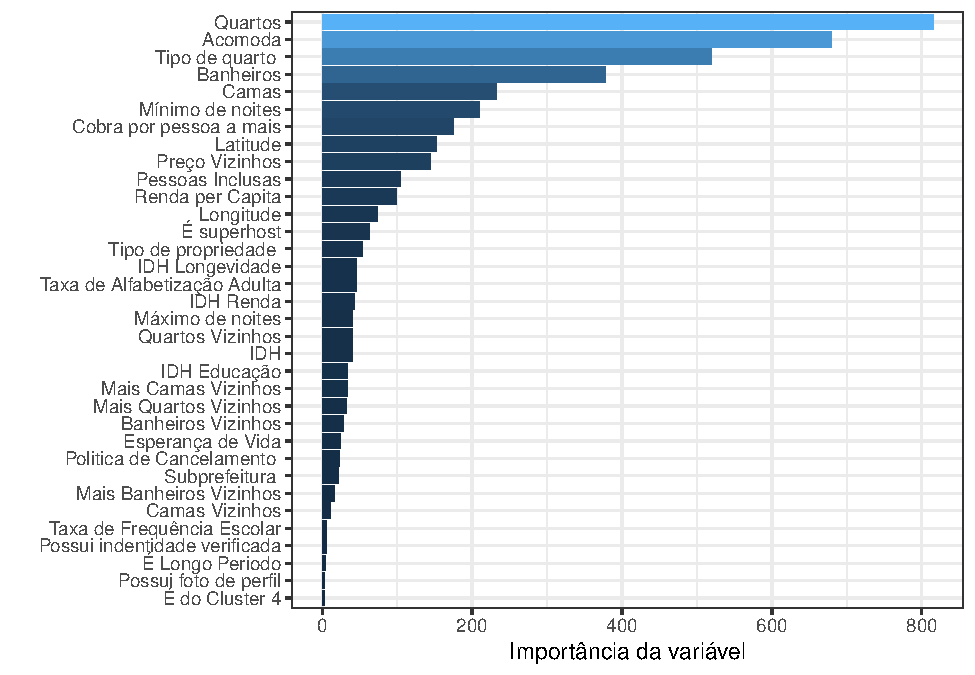
\includegraphics{00-TCC_files/figure-latex/imp_var_rf-1.pdf}
\caption{\label{imp_var_rf}Importância das variáveis no Random Forest}
\end{figure}

O modelo com os hiperparâmetros otimizados levou aproximadamente 1,17
segundos para treinar e a predição da base de treino levou
aproximadamente 0,13 segundos. Com a otimização, foi significativa a
redução da velocidade para a compilação do modelo.

Utilizando-se do modelo Random Forest com 50 árvores, haverá então 50
previsões para cada propriedade, resultado de cada árvore de decisão.
Como podemos verificar na Figura \ref{exemplo_pred}, há uma distribuição
das previsões de cada árvore para uma única propriedade, cujo valor real
de diária é de R\$105,00.

\begin{figure}
\centering
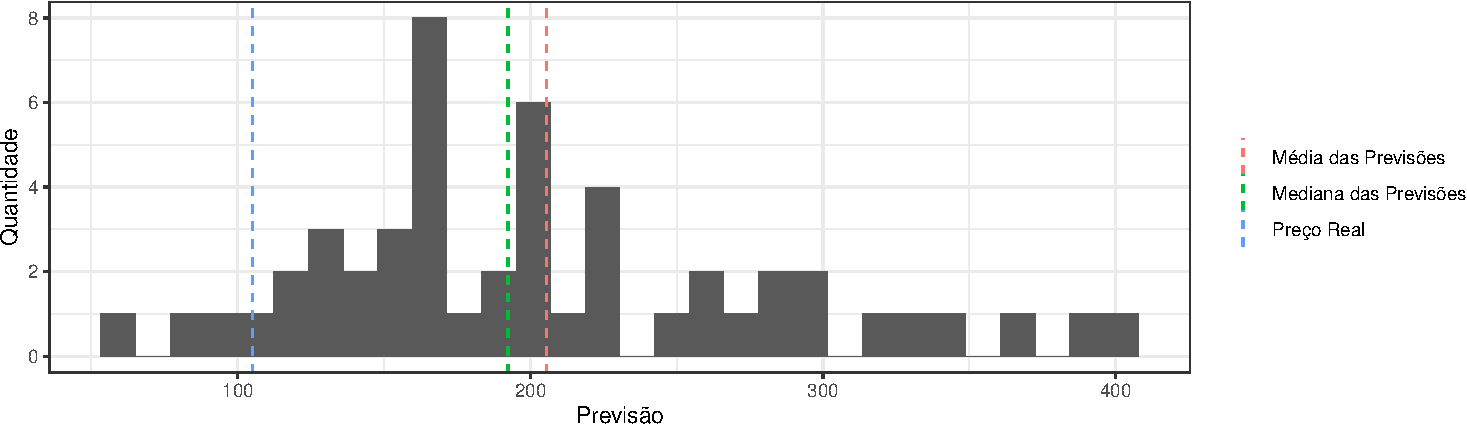
\includegraphics{00-TCC_files/figure-latex/exemplo_pred-1.pdf}
\caption{\label{exemplo_pred}Exemplo de previsão}
\end{figure}

Com isso, chegamos nos resíduos do Random Forest com Transformação
Inversa, pois foi utilizada a variável resposta com transformação
(melhor desempenho). Utilizou-se das médias das previsões das árvores
para cada propriedade, conforme Figura \ref{resid_rf_inv}.

\begin{table}

\caption{\label{tab:rf1_metricas}Estimativa do erro destransformado para o random forest otimizado}
\centering
\begin{tabular}[t]{l|r|r|r|r}
\hline
Base & REQM & EAM & EPAM & R2\\
\hline
Treino & 211,31 & 134,11 & 40,29 & 0,58\\
\hline
Teste & 246,58 & 161,32 & 50,88 & 0,38\\
\hline
\multicolumn{5}{l}{\textit{Fonte: } O próprio autor}\\
\end{tabular}
\end{table}

\begin{figure}
\centering
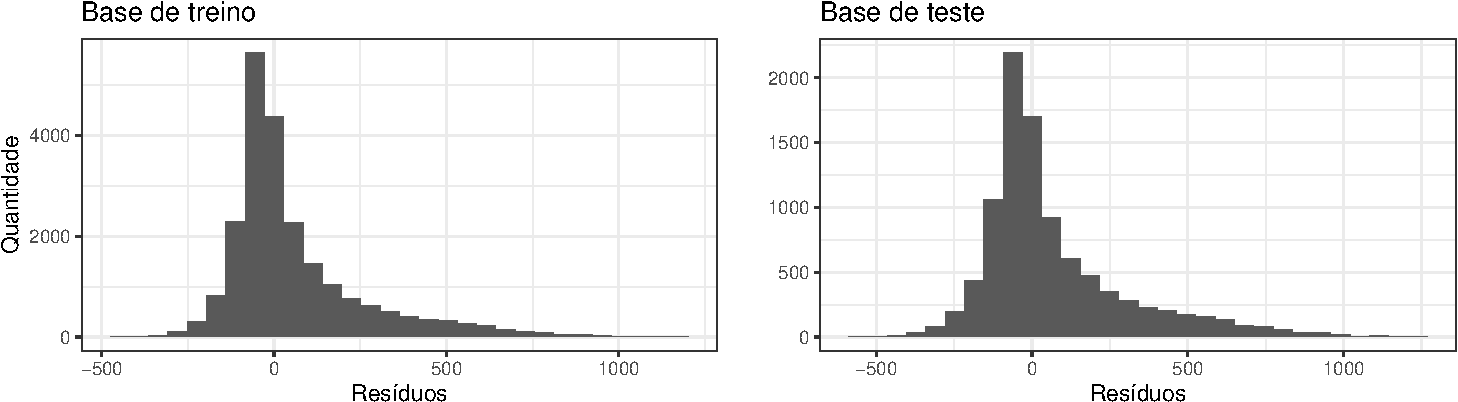
\includegraphics{00-TCC_files/figure-latex/resid_rf_inv-1.pdf}
\caption{\label{resid_rf_inv}Resíduos do Random Forest com Transformação
Inversa}
\end{figure}

Nas análises seguintes, será utilizada a métrica Erro Percentual
Absoluto Médio (EPAM) por representar o percentual de erro, invariante
quanto a escala.

De acordo com a Tabela \ref{tab:erro_test} aproximadamente 30\% das
previsões tiveram menos de R\$50 de erro e portanto, algumas
propriedades são fáceis de prever, enquanto outras são um pouco mais
difíceis.

De acordo com a Figura \ref{graf_resid_rf}, as duas primeiras categorias
(\(\le\) R\$101,00) não apresentam um nível confiável pelo alto valor do
EPAM.

\begin{figure}
\centering
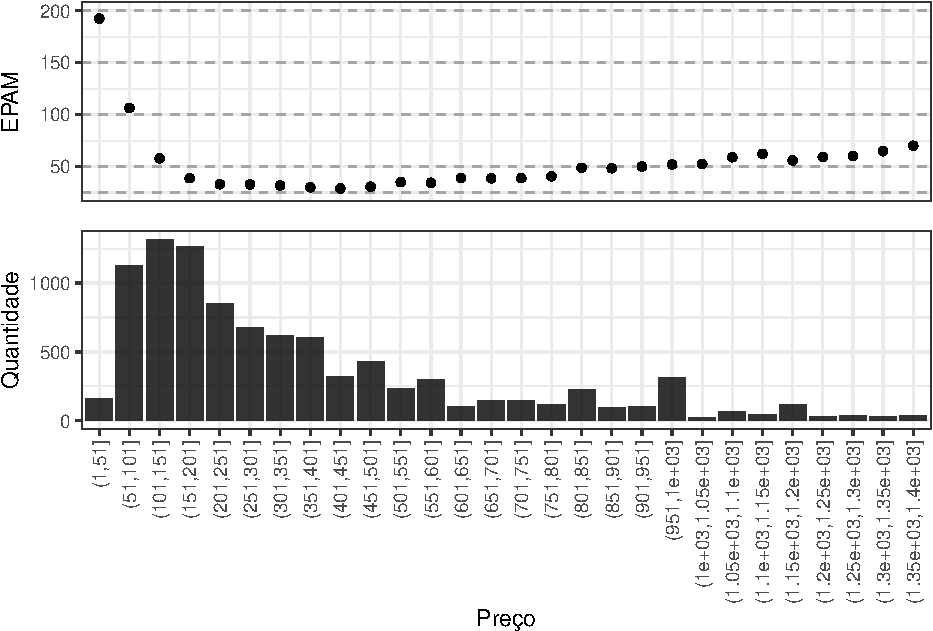
\includegraphics{00-TCC_files/figure-latex/graf_resid_rf-1.pdf}
\caption{\label{graf_resid_rf}Distribuição dos Resíduos do Random
Forest}
\end{figure}

\begin{table}

\caption{\label{tab:erro_test}Descrição do erro na base de teste}
\centering
\begin{tabular}[t]{l|r|r|r|r}
\hline
Erro Absoluto & Quantidade & Preço Mediano & Proporção & Proporção Acumulada\\
\hline
(0,25] & 1.366 & R\$   199,00 & 14,25 & 14,25\\
\hline
(25,50] & 1.450 & R\$   188,00 & 15,12 & 29,37\\
\hline
(50,100] & 2.251 & R\$   183,00 & 23,48 & 52,85\\
\hline
(100,200] & 2.140 & R\$   298,00 & 22,32 & 75,17\\
\hline
(200,400] & 1.345 & R\$   502,00 & 14,03 & 89,20\\
\hline
(400,800] & 893 & R\$   999,00 & 9,31 & 98,52\\
\hline
(800,1.6e+03] & 142 & R\$ 1.217,00 & 1,48 & 100,00\\
\hline
\multicolumn{5}{l}{\textit{Fonte: } O próprio autor}\\
\end{tabular}
\end{table}

Nas Figuras \ref{graf_resid_rf_acom}, \ref{graf_resid_rf_quartos} e
\ref{graf_resid_rf_tp_quarto} é feita uma análise mais detalhada quanto
ao resíduo do modelo na base de teste, onde é apresentado o erro,
separado pelas variáveis mais relevantes (Número máximo de hóspedes,
Quantidade de Quartos e Tipo de Quarto) pelas faixas de preço. É
possível notar que as propriedades pequenas e com preço baixo (\(\leq\)
R\$151) apresentam um alto erro, comparadas a propriedades maiores e de
preço mais elevado. É possível notar que o modelo, para estes casos,
tende a sugerir preços mais altos que os escolhidos pelo proprietário,
dando a entender que o imóvel esteja ``barato''.

\begin{figure}
\centering
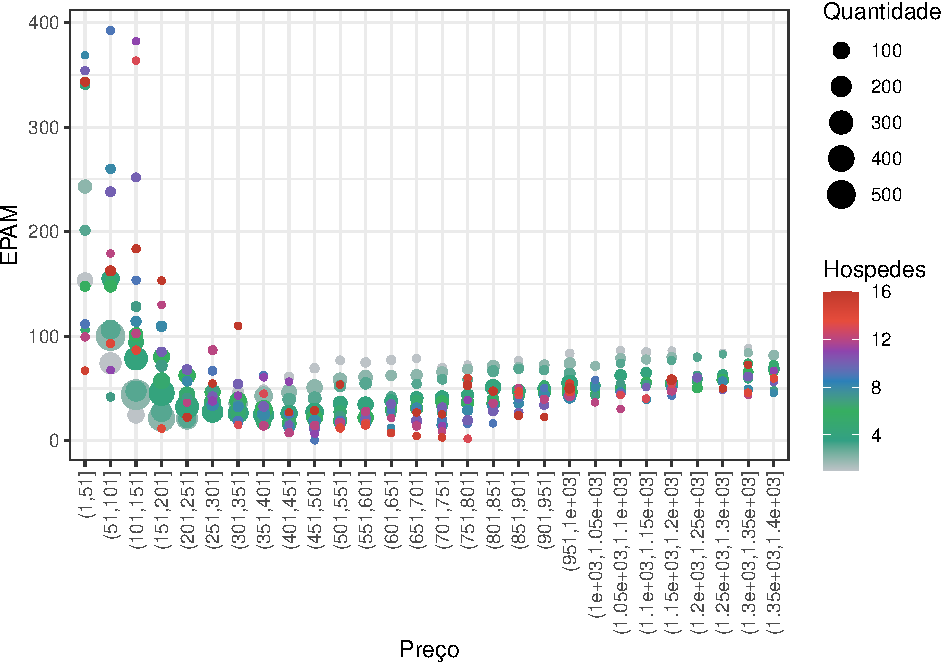
\includegraphics{00-TCC_files/figure-latex/graf_resid_rf_acom-1.pdf}
\caption{\label{graf_resid_rf_acom}Distribuição dos Resíduos do Random
Forest por quantidade de hóspedes}
\end{figure}

A variável \emph{Quartos}, uma das mais importantes no modelo de acordo
com a lista de significância, também é muito influenciada como podemos
notar na Figura \ref{graf_resid_rf_quartos}: um grande erro nas faixas
baixas de preço relacionadas a uma quantidade intermediária/grande de
quartos (de 5 a 10 quartos por propriedade).

\begin{figure}
\centering
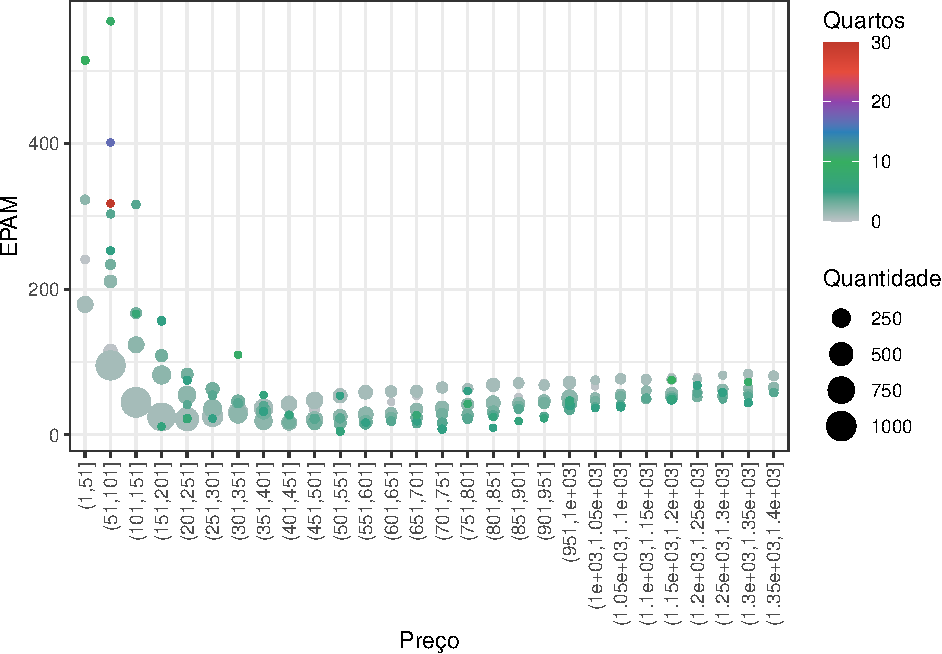
\includegraphics{00-TCC_files/figure-latex/unnamed-chunk-43-1.pdf}
\caption{\label{graf_resid_rf_quartos}Distribuição dos Resíduos do
Random Forest por quartos}
\end{figure}

De acordo com a Figura \ref{graf_resid_rf_tp_quarto}, a variável
\emph{Tipo de Quarto} também não se relaciona bem com as pequenas faixas
de preço. Além disso, a categoria ``Entire home/apt'' (Casa/Apartamento
Inteiro) apresenta um erro destoante das demais para as propriedades
mais baratas, o que pode ser uma dificuldade do modelo ao identifica-la
ou uma classificação errada na base de dados.

\begin{figure}
\centering
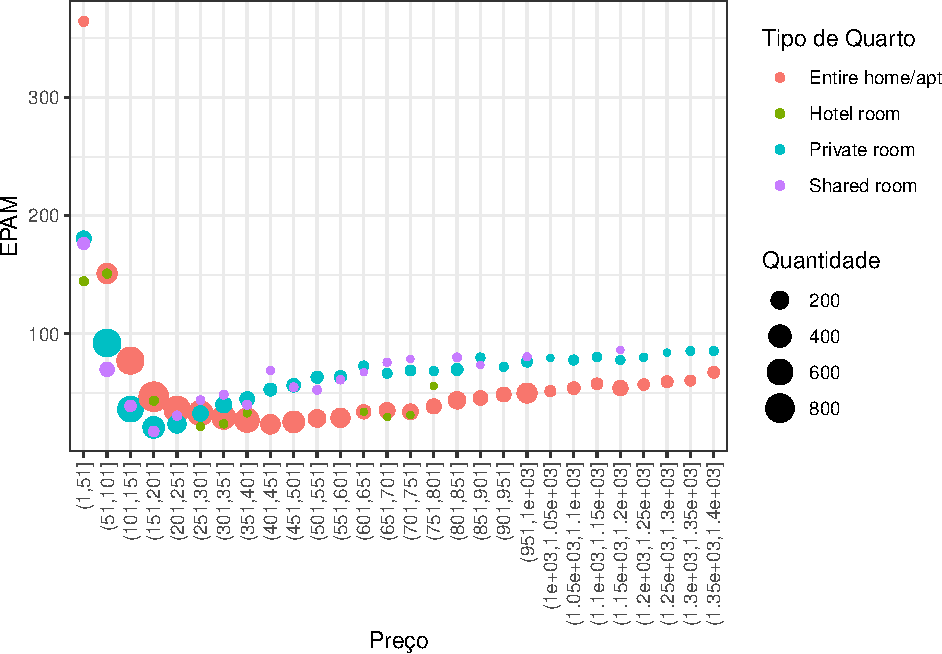
\includegraphics{00-TCC_files/figure-latex/graf_resid_rf_tp_quarto-1.pdf}
\caption{\label{graf_resid_rf_tp_quarto}Distribuição dos Resíduos do
Random Forest por tipo de quarto}
\end{figure}

\hypertarget{comparativo}{%
\subsection{Comparativo}\label{comparativo}}

Comparou-se o desempenho dos modelos preditivos a partir de seus
resultados e características de seus algoritmos. Como o Random Forest é
um algoritmo custoso computacionalmente, foram utilizadas os seguintes
algoritmos/modelos para comparação: média dos 15 vizinhos mais próximos
e um modelo linear.

Utilizando a base de treino, o Random Forest com otimização teve um erro
percentual absoluto médio de 40,29\% (50,90\% na base de teste) em
comparação ao modelo sem otimização (23,98\%). Para o modelo
\emph{baseline} foi obtido um EPAM de 71,96\% (74,18\% na base de teste)
e para o modelo linear melhor ajustado 54,23\% (55,65\% na base de
teste). Cabe ressaltar que a diferença de todas as métricas de erros
utilizadas não indica uma diferença significativa entre os modelos não
lineares (árvores) e modelo lineares.

\begin{table}

\caption{\label{tab:comp_erro}Comparativo de erro entre os modelos na base de treino}
\centering
\begin{tabular}[t]{l|r|r|r|r}
\hline
Modelo & EAM & EPAM & R2 & REQM\\
\hline
Modelo Baseline & 205,82 & 71,96 & 0,06 & 302,82\\
\hline
Seleção Manual & 166,80 & 54,23 & 0,32 & 251,93\\
\hline
LASSO & 167,52 & 54,46 & 0,31 & 253,79\\
\hline
Random Forest Base & 87,83 & 23,98 & 0,84 & 148,54\\
\hline
Random Forest Otimizado & 134,11 & 40,29 & 0,58 & 211,31\\
\hline
\multicolumn{5}{l}{\textit{Fonte: } O próprio autor}\\
\end{tabular}
\end{table}

\begin{table}

\caption{\label{tab:comp_erro_teste}Comparativo de erro entre os modelos na base de teste}
\centering
\begin{tabular}[t]{l|r|r|r|r}
\hline
Modelo & EAM & EPAM & R2 & REQM\\
\hline
Modelo Baseline & 210,21 & 74,18 & 0,06 & 306,77\\
\hline
Seleção Manual & 169,16 & 55,66 & 0,32 & 254,49\\
\hline
LASSO & 169,83 & 55,95 & 0,31 & 256,35\\
\hline
Random Forest Base & 159,41 & 50,10 & 0,39 & 243,83\\
\hline
Random Forest Otimizado & 161,32 & 50,88 & 0,38 & 246,58\\
\hline
\multicolumn{5}{l}{\textit{Fonte: } O próprio autor}\\
\end{tabular}
\end{table}

Com uma breve comparação das variáveis de acordo com a importância, o
\emph{tipo de quarto}, seja considerando a variável toda ou alguma
categoria, mostrou-se relevante para todos os modelos utilizados no
trabalho, independente do modo de seleção. Variáveis que dimensionam o
tamanho da propriedade como, por exemplo, quantidade de quartos,
quantidade de banheiros e capacidade de pessoas acomodadas, foram bem
presentes nos modelos de Regressão Linear e Random Forest. Já no modelo
de Random Forest com otimização dos parâmetros, variáveis utilizadas
para complementar o trabalho, como latitude e renda per capita, foram
relevantes, nos dando a ideia de que, dependendo do bairro, há uma
influência no valor da propriedade oferecida.

Os resultados obtidos colocam como melhor modelo o Random Forest sem
otimização dos hiperparâmetros para a previsão da base de dados
utilizada, dado que se trata de um modelo não-paramétrico, e por isso,
dentre os modelos utilizados, é o que mais se adequa aos dados
fornecidos. Porém, analisando as métricas de erro e comparando os
resultados entre treino e teste, é possível notar grande discrepância de
erro entre as bases teste e treino, e por isso, será considerado o
modelo otimizado, por apresentar um menor grau de sobreajuste e com uma
maior estabilidade. Os modelos baseados em Random Forest apresentam um
erro relativamente menor comparado aos modelos lineares.

\hypertarget{conclusuxe3o}{%
\chapter{Conclusão}\label{conclusuxe3o}}

O objetivo principal deste trabalho foi desenvolver um modelo preditivo
para a recomendação de preços de diárias de propriedades localizadas no
Rio de Janeiro utilizando o algoritmo Random Forest. Foram apresentados
os principais conteúdos teóricos dos algoritmos utilizados, bem como os
principais conceitos para entendimento do tema e aplicações. O modelo
Random Forest com otimização dos parâmetros obteve um melhor desempenho
dentre os modelos apresentados. Por um outro lado, a elaboração de
relações lineares é um método simples e que garante resultados de
previsão precisos para um específico conjunto de dados. Contudo, podem
existir outros modelos lineares, como o generalizados, que forneçam
resultados mais acurados para os dados utilizados.

Dentre as limitações encontradas nesse trabalho, há a carência de uma
análise estatística preliminar mais profunda das variáveis de acordo com
a faixa de preço, pois nos resultados foram encontrados grandes erros de
variáveis regressoras relacionados a pequenas faixas da variável
resposta.

Quanto aos métodos de seleção de variáveis, não houveram mudanças
significativas nas métricas dos erros, mas cabe ressaltar que a base de
dados utilizada não possui uma grande quantidade de variáveis, e por
isso foi possível fazer uma avaliação mais minuciosa sobre as variáveis
que entrariam ou sairiam do modelo, sendo um trabalho altamente custoso
para bases com muitas variáveis. Sendo assim, a técnica apresentou bons
resultados, sendo muito eficaz para seleção de variáveis e resolvendo
problemas de multicolinearidade.

Como sugestão de trabalhos futuros, há a possibilidade de estudar sobre
a criação de novas variáveis, como, por exemplo, a distância até a praia
mais próxima, utilizando uma base de dados disponibilizada pelo
INEA\footnote{\url{http://www.inea.rj.gov.br/wp-content/uploads/2018/12/Coordenadas-Geogr\%C3\%A1ficas-das-Esta\%C3\%A7\%C3\%B5es-de-Amostragem-Praias.pdf}}.
Além de testar modelos estatísticos mais adequados como os Modelos
Lineares Generalizados, outros algoritmos de aprendizagem supervisionado
como o booting e fazer uma análise mais profunda com relação ao erro de
classificação das propriedades.

O trabalho foi desenvolvido utilizando a linguagem de programação R e
está disponível em um repositório aberto no
github.\footnote{\url{https://github.com/dobraga/TCC}}

Foi utilizada a tecnologia shiny, que tem como o objetivo a criação de
aplicações web na linguagem R. Criou-se uma interface intuitiva e de
fácil acesso. Nesta interface, o usuário consegue manipular as
características dos imóveis (como quantidade de quartos,quantidade de
pessoas,\ldots{}) e principalmente o local do mesmo, como podemos
verificar na Figura \ref{fig:dash1}. Após seleção das características e
do local, entrando na aba ``Preço Proposto'', representada na Figura
\ref{fig:dash2}, podemos clicar no botão ``Preve-ja'', para termos as
sugestões, considerando a média e a mediana das previsões das árvores e
sua respectiva distribuição.

\begin{figure}
\centering
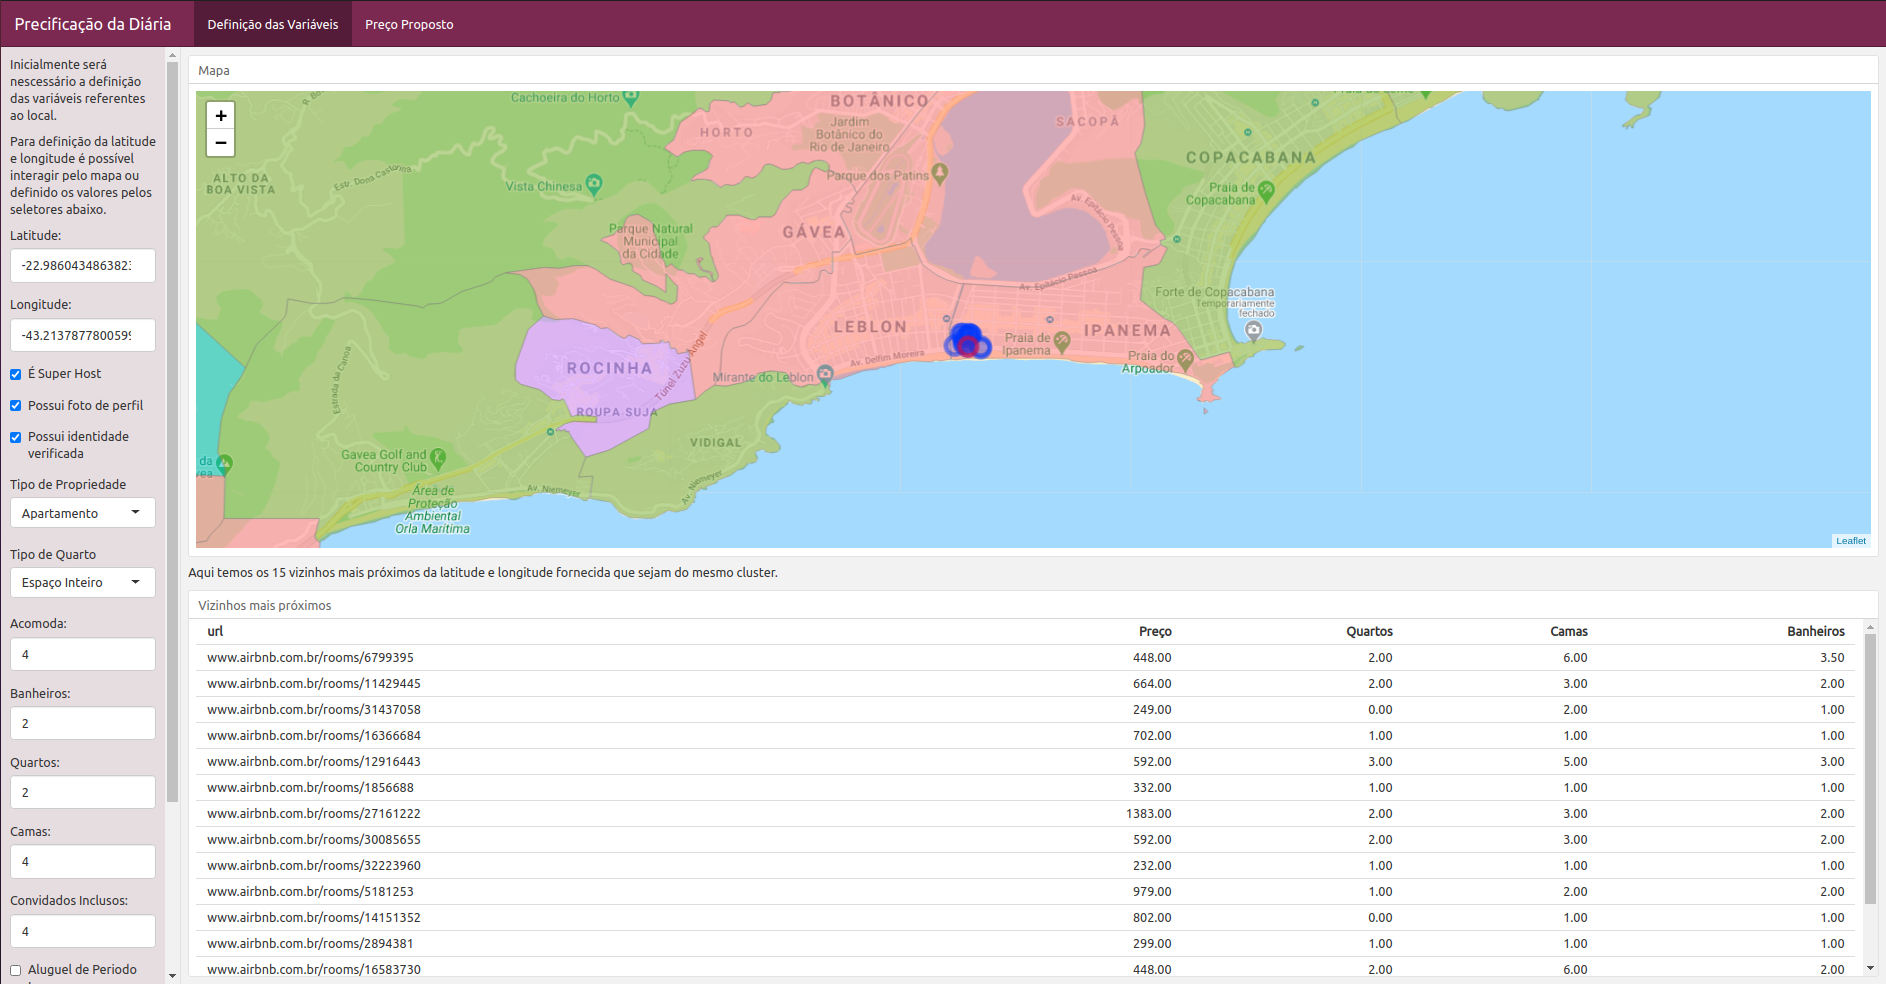
\includegraphics[width=\textwidth,height=0.3\textheight]{../fig/dash1.png}
\caption{Dashboard - Definição das Variáveis\label{fig:dash1}}
\end{figure}

\begin{figure}
\centering
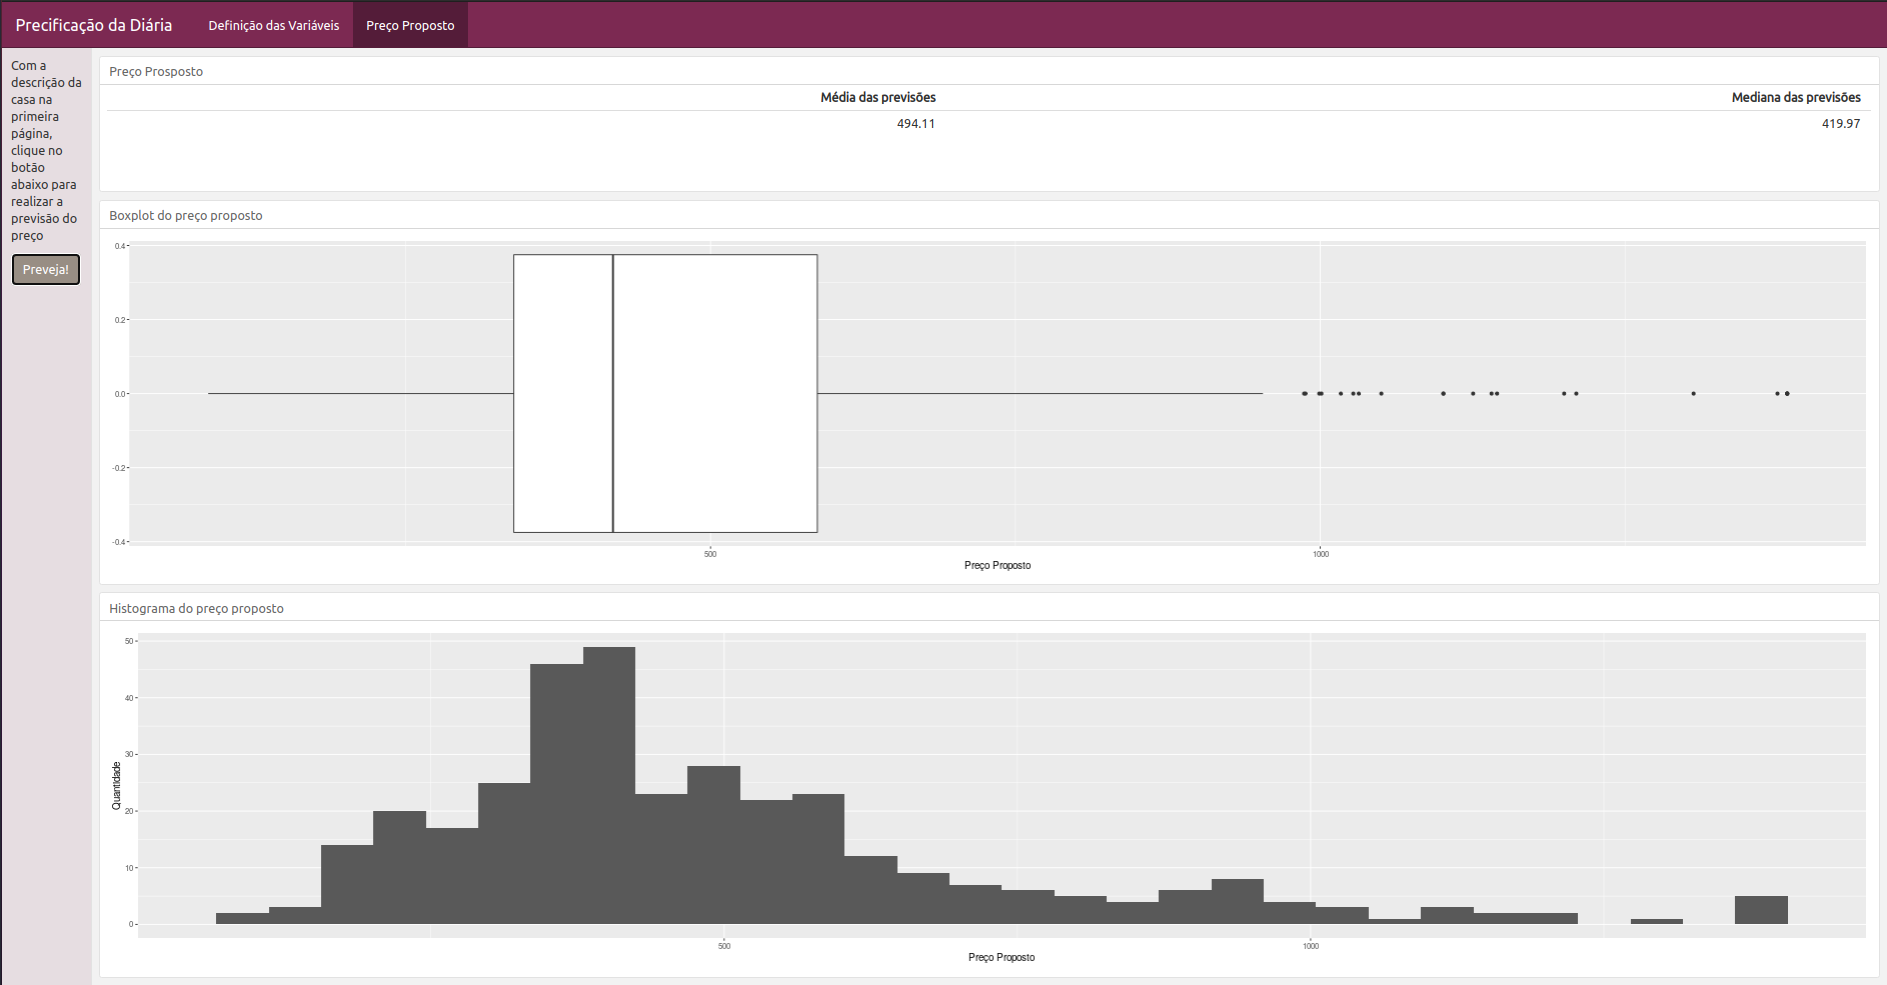
\includegraphics[width=\textwidth,height=0.3\textheight]{../fig/dash2.png}
\caption{Dashboard - Preço Proposto\label{fig:dash2}}
\end{figure}

A comparação dos modelos preditivos proposta foi finalizada atendendo ao
objetivo geral.

\newpage

\hypertarget{referuxeancias}{%
\chapter*{REFERÊNCIAS}\label{referuxeancias}}
\addcontentsline{toc}{chapter}{REFERÊNCIAS}

\hypertarget{refs}{}
\leavevmode\hypertarget{ref-airbnbperiodolongo}{}%
AIRBNB. \textbf{Quais as diferenças entre as hospedagens de longo e
curto prazo?}, 2018.

\leavevmode\hypertarget{ref-inside}{}%
\_\_\_. \textbf{Inside
Airbnb}\url{http://insideairbnb.com/get-the-data.html},, 2020a.

\leavevmode\hypertarget{ref-precoairbnb}{}%
\_\_\_. \textbf{Como devo escolher o preço do meu anúncio?}, 2020b.

\leavevmode\hypertarget{ref-baker2005administraccao}{}%
BAKER, A. S., Michel e Marques. \textbf{Administração de marketing}.
Traducao. {[}s.l.{]} Elsevier, 2005.

\leavevmode\hypertarget{ref-balck2015empirical}{}%
BALCK, D., B e Cracau. Empirical analysis of customer motives in the
shareconomy: a cross-sectoral comparison (Working Paper No. 2/2015).
\textbf{Retrieved from the Faculty of Economics and Management,
Otto-von-Guericke University Magdeburg}, 2015.

\leavevmode\hypertarget{ref-becerra2013being}{}%
BECERRA, J. E S., Manuel e Santaló. Being better vs. being different:
Differentiation, competition, and pricing strategies in the Spanish
hotel industry. \textbf{Tourism management}, v. 34, p. 71--79, 2013.

\leavevmode\hypertarget{ref-belk2014you}{}%
BELK, R. You are what you can access: Sharing and collaborative
consumption online. \textbf{Journal of business research}, v. 67, n. 8,
p. 1595--1600, 2014.

\leavevmode\hypertarget{ref-botsman2011meu}{}%
BOTSMAN, R., Rachel e ROGERS. O que é meu é seu: como o consume
colaborativo pode mudar o nosso mundo. \textbf{Porto Alegre: Booksman},
2011.

\leavevmode\hypertarget{ref-botsman2010s}{}%
BOTSMAN, R., Rachel e Rogers. What's mine is yours. \textbf{The rise of
collaborative consumption}, 2010.

\leavevmode\hypertarget{ref-box1964analysis}{}%
BOX, D. R., George EP e Cox. An analysis of transformations.
\textbf{Journal of the Royal Statistical Society: Series B
(Methodological)}, v. 26, n. 2, p. 211--243, 1964.

\leavevmode\hypertarget{ref-breiman1984j}{}%
BREIMAN, L. J. H. Friedman, RA Olshen, and C. \textbf{J. Stone}, 1984.

\leavevmode\hypertarget{ref-breiman1996bagging}{}%
BREIMAN, L. Bagging predictors. \textbf{Machine learning}, v. 24, n. 2,
p. 123--140, 1996.

\leavevmode\hypertarget{ref-breiman2001random}{}%
\_\_\_. Random forests. \textbf{Machine learning}, v. 45, n. 1, p.
5--32, 2001.

\leavevmode\hypertarget{ref-chatterjee2006analysis}{}%
CHATTERJEE, A. E P., S e Hadi. Analysis of collinear data.
\textbf{Regression analysis by example}, p. 143--174, 2006.

\leavevmode\hypertarget{ref-chen2010application}{}%
CHEN, C.-F.; ROTHSCHILD, R. An application of hedonic pricing analysis
to the case of hotel rooms in Taipei. \textbf{Tourism Economics}, v. 16,
n. 3, p. 685--694, 2010.

\leavevmode\hypertarget{ref-cohen2015self}{}%
COHEN, A., Molly e Sundararajan. Self-regulation and innovation in the
peer-to-peer sharing economy. \textbf{U. Chi. L. Rev. Dialogue}, v. 82,
p. 116, 2015.

\leavevmode\hypertarget{ref-datario}{}%
DATA.RIO. \textbf{Índice de Desenvolvimento Humano (IDH) Municipal, por
ordem de IDH, segundo os Bairros ou grupo de Bairros, no Município do
Rio de Janeiro em 1991/2000}, 2020.

\leavevmode\hypertarget{ref-eckhardt2015sharing}{}%
ECKHARDT, F., Giana M e Bardhi. The sharing economy isn't about sharing
at all. \textbf{Harvard business review}, v. 28, n. 1, p. 2015, 2015.

\leavevmode\hypertarget{ref-efron1994introduction}{}%
EFRON, R. J., Bradley e Tibshirani. \textbf{An introduction to the
bootstrap}. Traducao. {[}s.l.{]} CRC press, 1994.

\leavevmode\hypertarget{ref-fontanaestudo}{}%
FONTANA, M., A e Naldi. \textbf{Estudo de Comparação de Métodos para
Estimação de Números de Grupos em Problemas de Agrupamento de Dados.
2009. Universidade de São Paulo}. {[}s.l.{]} ISSN-0103-2569, 2009.

\leavevmode\hypertarget{ref-friedman2000additive}{}%
FRIEDMAN, T. E T., Jerome e Hastie. Additive logistic regression: a
statistical view of boosting (with discussion and a rejoinder by the
authors). \textbf{The annals of statistics}, v. 28, n. 2, p. 337--407,
2000.

\leavevmode\hypertarget{ref-friedman2001elements}{}%
\_\_\_. \textbf{The elements of statistical learning}. Traducao.
{[}s.l.{]} Springer series in statistics New York, 2001. v. 1

\leavevmode\hypertarget{ref-friedman2010regularization}{}%
\_\_\_. Regularization paths for generalized linear models via
coordinate descent. \textbf{Journal of statistical software}, v. 33, n.
1, p. 1, 2010.

\leavevmode\hypertarget{ref-gansky2010mesh}{}%
GANSKY, L. \textbf{The mesh: Why the future of business is sharing}.
Traducao. {[}s.l.{]} Penguin, 2010.

\leavevmode\hypertarget{ref-gutt2015sharing}{}%
GUTT, P., Dominik e Herrmann. Sharing means caring? Hosts' price
reaction to rating visibility. 2015.

\leavevmode\hypertarget{ref-guttentag2015airbnb}{}%
GUTTENTAG, D. Airbnb: disruptive innovation and the rise of an informal
tourism accommodation sector. \textbf{Current issues in Tourism}, v. 18,
n. 12, p. 1192--1217, 2015.

\leavevmode\hypertarget{ref-heo2016sharing}{}%
HEO, Y. E OUTROS. Sharing economy and prospects in tourism research.
\textbf{Annals of tourism Research}, v. 58, p. 166--170, 2016.

\leavevmode\hypertarget{ref-horngren2008contabilidade}{}%
HORNGREN, S. M. E F., Charles T e Datar. \textbf{Contabilidade de
custos}. Traducao. {[}s.l.{]} Pearson Prentice Hall, 2008.

\leavevmode\hypertarget{ref-hung2010pricing}{}%
HUNG, J.-K. E W., Wei-Ting e Shang. Pricing determinants in the hotel
industry: Quantile regression analysis. \textbf{International Journal of
Hospitality Management}, v. 29, n. 3, p. 378--384, 2010.

\leavevmode\hypertarget{ref-huse2006estimaccao}{}%
HUSE, A., Cristian e Salvo. Estimação e identificação de demanda e de
oferta. \textbf{Métodos quantitativos em defesa da concorrência e
regulação econômica}, 2006.

\leavevmode\hypertarget{ref-ikkala2014defining}{}%
IKKALA, A., Tapio e Lampinen. \textbf{Defining the price of hospitality:
networked hospitality exchange via Airbnb}Proceedings of the companion
publication of the 17th ACM conference on Computer supported cooperative
work \& social computing. \textbf{Anais}\ldots{}2014

\leavevmode\hypertarget{ref-jain1999data}{}%
JAIN, M. N. E F., Anil K e Murty. Data clustering: a review. \textbf{ACM
computing surveys (CSUR)}, v. 31, n. 3, p. 264--323, 1999.

\leavevmode\hypertarget{ref-kaplan2010users}{}%
KAPLAN, M., Andreas M e Haenlein. Users of the world, unite! The
challenges and opportunities of Social Media. \textbf{Business
horizons}, v. 53, n. 1, p. 59--68, 2010.

\leavevmode\hypertarget{ref-karlsson2016someone}{}%
KARLSSON, S. E OUTROS, Logi e Dolnicar. Someone's been sleeping in my
bed. \textbf{Annals of Tourism Research}, v. 58, p. 159--162, 2016.

\leavevmode\hypertarget{ref-kotler2007principios}{}%
KOTLER, G., Philip e Armstrong. \textbf{Princípios de marketing}.
Traducao. {[}s.l.{]} Pearson Prentice Hall, 2007.

\leavevmode\hypertarget{ref-lavaquial2015cocriando}{}%
LAVAQUIAL, A. \textbf{Cocriando Valor na economia colaborativa sob a
perspectiva da Lógica Dominante de Serviço: o caso. Airbnb}. {[}s.l.{]}
Dissertação (Mestrado)-UFRJ/COPPE, Rio de Janeiro, 2015.

\leavevmode\hypertarget{ref-li2015agent}{}%
LI, A. E Z., Jun e Moreno. Agent behavior in the sharing economy:
Evidence from Airbnb. \textbf{Ross School of Business Working Paper
Series}, v. 1298, p. 2015, 2015.

\leavevmode\hypertarget{ref-loboeconomia}{}%
LOBO, Y. S. Economia colaborativa e Airbnb: reflexões urbano-turísticas
a partir de São Paulo e Rio de Janeiro. 2018.

\leavevmode\hypertarget{ref-martinez2019sequential}{}%
MARTÍNEZ-MUÑOZ, G. Sequential Training of Neural Networks with Gradient
Boosting. \textbf{arXiv preprint arXiv:1909.12098}, 2019.

\leavevmode\hypertarget{ref-masiero2015demand}{}%
MASIERO, J. L. E L., Lorenzo e Nicolau. A demand-driven analysis of
tourist accommodation price: A quantile regression of room bookings.
\textbf{International Journal of Hospitality Management}, v. 50, p.
1--8, 2015.

\leavevmode\hypertarget{ref-murphy2012probabilistic}{}%
MURPHY, K. P. A Probabilistic Perspective. \textbf{Text book}, 2012.

\leavevmode\hypertarget{ref-neter1989applied}{}%
NETER, W. E K., John e Wasserman. Applied linear regression models.
1989.

\leavevmode\hypertarget{ref-opitz1999popular}{}%
OPITZ, R., David e Maclin. Popular ensemble methods: An empirical study.
\textbf{Journal of artificial intelligence research}, v. 11, p.
169--198, 1999.

\leavevmode\hypertarget{ref-pesonen2017peer}{}%
PESONEN, I., Juho e Tussyadiah. Peer-to-peer accommodation: drivers and
user profiles. \emph{In}: \textbf{Collaborative Economy and Tourism}.
Traducao. {[}s.l.{]} Springer, 2017. p. 285--303.

\leavevmode\hypertarget{ref-petrini2012degree}{}%
PETRINI, R. A. P. E P., Juliana e Dias. Degree of multicollinearity and
variables involved in linear dependence in additive-dominant models.
\textbf{Pesquisa Agropecuária Brasileira}, v. 47, n. 12, p. 1743--1750,
2012.

\leavevmode\hypertarget{ref-quinby2014share}{}%
QUINBY, M., D e Gasdia. Share this! Private accommodation and the rise
of the new gen renters. \textbf{Report. PhoCusWright}, 2014.

\leavevmode\hypertarget{ref-robert2014machine}{}%
ROBERT, C. \textbf{Machine learning, a probabilistic perspective}Taylor
\& Francis,, 2014.

\leavevmode\hypertarget{ref-schapire1999brief}{}%
SCHAPIRE, R. E. \textbf{A brief introduction to boosting}Ijcai.
\textbf{Anais}\ldots{}1999

\leavevmode\hypertarget{ref-sundararajan2014peer}{}%
SUNDARARAJAN, A. Peer-to-peer businesses and the sharing (collaborative)
economy: Overview, economic effects and regulatory issues.
\textbf{Written testimony for the hearing titled The Power of
Connection: Peer to Peer Businesses}, 2014.

\leavevmode\hypertarget{ref-tang2015neighborhood}{}%
TANG, K., Emily e Sangani. \textbf{Neighborhood and price prediction for
San Francisco Airbnb listings}Stanford Univ., Stanford, CA, USA, Tech.
Rep,, 2015.

\leavevmode\hypertarget{ref-tibshirani1996regression}{}%
TIBSHIRANI, R. Regression shrinkage and selection via the lasso.
\textbf{Journal of the Royal Statistical Society: Series B
(Methodological)}, v. 58, n. 1, p. 267--288, 1996.

\leavevmode\hypertarget{ref-tussyadiah2016strategic}{}%
TUSSYADIAH, I. P. Strategic self-presentation in the sharing economy:
Implications for host branding. \emph{In}: \textbf{Information and
Communication Technologies in Tourism 2016}. Traducao. {[}s.l.{]}
Springer, 2016. p. 695--708.

\leavevmode\hypertarget{ref-werkema1996analise}{}%
WERKEMA, S., Maria Cristina Catarino e Aguiar. \textbf{Análise de
regressão: como entender o relacionamento entre as variáveis de um
processo}. Traducao. {[}s.l.{]} UFMG, Escola de Engenharia, Fundação
Christiano Ottoni, 1996.

\leavevmode\hypertarget{ref-woodruff1997customer}{}%
WOODRUFF, R. B. Customer value: the next source for competitive
advantage. \textbf{Journal of the academy of marketing science}, v. 25,
n. 2, p. 139, 1997.

\leavevmode\hypertarget{ref-wright2015ranger}{}%
WRIGHT, A., Marvin N e Ziegler. ranger: A fast implementation of random
forests for high dimensional data in C++ and R. \textbf{arXiv preprint
arXiv:1508.04409}, 2015.

\hypertarget{apuxeandice-a}{%
\chapter*{APÊNDICE A}\label{apuxeandice-a}}
\addcontentsline{toc}{chapter}{APÊNDICE A}

A Tabela \ref{tab:cluster_bairros} mostra o agrupamento de bairros
utilizando o k-means.

\begin{table}

\caption{\label{tab:cluster_bairros}Clusters de bairros}
\centering
\begin{tabular}[t]{r|>{\raggedright\arraybackslash}p{15cm}}
\hline
cluster & bairros\\
\hline
1 & Gávea, Ipanema, Jardim Botânico, Lagoa, Leblon, Barra da Tijuca, Joá\\
\hline
2 & Botafogo, Copacabana, Flamengo, Glória, Humaitá, Laranjeiras, Leme, São Conrado, Urca, Vidigal, Grumari, Recreio dos Bandeirantes, Alto da Boa Vista, Grajaú, Maracanã, Tijuca, Méier, Jardim Guanabara\\
\hline
3 & Centro, Cidade Nova, Lapa, Paquetá, Rio Comprido, Santa Teresa, Catete, Cosme Velho, Anil, Freguesia (Jacarepaguá), Itanhangá, Praça Seca, Pechincha, Taquara, Vila Valqueire, Jardim Sulacap, Campo dos Afonsos, Deodoro, Vila Militar, Andaraí, Praça da Bandeira, Vila Isabel, Abolição, Água Santa, Cachambi, Del Castilho, Encantado, Engenho de Dentro, Engenho Novo, Higienópolis, Jacaré, Lins de Vasconcelos, Maria da Graça, Riachuelo, Rocha, Sampaio, Todos os Santos, Bonsucesso, Bancários, Cacuia, Cocotá, Freguesia (Ilha), Moneró, Olaria, Pitangueiras, Portuguesa, Praia da Bandeira, Ramos, Ribeira, Zumbi, Campinho, Irajá, Vila da Penha, Vila Kosmos, Vista Alegre\\
\hline
4 & São Cristóvão, Benfica, Caju, Catumbi, Estácio, Gamboa, Mangueira, Santo Cristo, Saúde, Vasco da Gama, Camorim, Cidade de Deus, Curicica, Gardênia Azul, Jacarepaguá, Tanque, Vargem Grande, Vargem Pequena, Bangu, Gericinó, Magalhães Bastos, Padre Miguel, Realengo, Santíssimo, Senador Camará, Vila Kennedy, Barra de Guaratiba, Campo Grande, Cosmos, Guaratiba, Inhoaíba, Paciência, Pedra de Guaratiba, Santa Cruz, Senador Vasconcelos, Sepetiba, Jacarezinho, Manguinhos, Piedade, Pilares, São Francisco Xavier, Cidade Universitária, Galeão, Jardim Carioca, Maré, Tauá, Acari, Anchieta, Barros Filho, Bento Ribeiro, Brás de Pina, Cavalcanti, Cascadura, Coelho Neto, Colégio, Complexo do Alemão, Cordovil, Costa Barros, Engenheiro Leal, Engenho da Rainha, Guadalupe, Honório Gurgel, Inhaúma, Jardim América, Madureira, Marechal Hermes, Osvaldo Cruz, Parada de Lucas, Parque Anchieta, Parque Colúmbia, Pavuna, Penha, Penha Circular, Quintino Bocaiúva, Ricardo de Albuquerque, Rocha Miranda, Tomás Coelho, Turiaçu, Vaz Lobo, Vicente de Carvalho, Vigário Geral, Rocinha\\
\hline
\multicolumn{2}{l}{\textit{Fonte: } O próprio autor}\\
\end{tabular}
\end{table}

A Tabela \ref{tab:desc_variaveis} descreve todas as variáveis utilizadas
na modelagem.

\begin{table}

\caption{\label{tab:desc_variaveis}Variáveis na base}
\centering
\begin{tabular}[t]{r|l|l|l}
\hline
Nº & Variável & Descrição & Origem\\
\hline
1 & id & Id gerado para identificar o imóvel & Airbnb\\
\hline
2 & host\_is\_superhost & Anfitriões experientes & Airbnb\\
\hline
3 & host\_has\_profile\_pic & Anfitriões com foto no perfil & Airbnb\\
\hline
4 & host\_identity\_verified & Anfitriões com identidade verificada & Airbnb\\
\hline
5 & neighbourhood\_cleansed & Bairro da Propriedade & Airbnb\\
\hline
6 & latitude & Latitude da propriedade & Airbnb\\
\hline
7 & longitude & Longitude da propriedade & Airbnb\\
\hline
8 & property\_type & Tipo de propriedade & Airbnb\\
\hline
9 & room\_type & Tipo de quarto & Airbnb\\
\hline
10 & accommodates & Número máximo de hóspedes & Airbnb\\
\hline
11 & bathrooms & Banheiros na propriedade & Airbnb\\
\hline
12 & bedrooms & Quartos na propriedade & Airbnb\\
\hline
13 & beds & Camas na propriedade & Airbnb\\
\hline
14 & guests\_included & Total de hóspedes inclusos na diária & Airbnb\\
\hline
15 & minimum\_nights & Quantidade Mínima de Noites & Airbnb\\
\hline
16 & maximum\_nights & Quantidade Máxima de Noites & Airbnb\\
\hline
17 & fl\_periodo\_longo & É Aluguel de Período Longo & Criada\\
\hline
18 & cancellation\_policy & Política de cancelamento & Airbnb\\
\hline
19 & zona & Zona da Propriedade & Data.RIO\\
\hline
20 & subprefeitura & Pequenos distritos & Data.RIO\\
\hline
21 & esperanca\_vida & Esperança de Vida do Bairro & Data.RIO\\
\hline
22 & tx\_alfabetizacao\_adulta & Taxa de Alfabetização Adulta & Data.RIO\\
\hline
23 & tx\_frequencia\_escolar & Taxa de Frequência Escolar & Data.RIO\\
\hline
24 & renda\_per\_capita & Renda per capita & Data.RIO\\
\hline
25 & idh\_longevidade & IDH de Longevidade & Data.RIO\\
\hline
26 & idh\_educacao & IDH de Educação & Data.RIO\\
\hline
27 & idh\_renda & IDH de Renda & Data.RIO\\
\hline
28 & idh & IDH & Data.RIO\\
\hline
29 & cluster & Cluster & Criada\\
\hline
30 & cluster\_4 & Bairro do cluster 4 & Criada\\
\hline
31 & price & Preço para alugar a propriedade & Airbnb\\
\hline
32 & fl\_extra\_people & Cobrança por pessoa a mais & Criada\\
\hline
33 & price\_near & Mediana do preço dos 15 vizinhos próx. & Criada\\
\hline
34 & bedrooms\_near & Mediana do nº de quartos dos 15 vizinhos próx. & Criada\\
\hline
35 & beds\_near & Mediana do nº de camasdos 15 vizinhos próx. & Criada\\
\hline
36 & bathrooms\_near & Mediana do nº de banheiros dos 15 vizinhos próx. & Criada\\
\hline
37 & fl\_mais\_banheiros & Mais banheiros que os 15 vizihos próx. & Criada\\
\hline
38 & fl\_mais\_quartos & Mais quartos que os 15 vizihos próx. & Criada\\
\hline
39 & fl\_mais\_camas & Mais camas que os 15 vizihos próx. & Criada\\
\hline
\multicolumn{4}{l}{\textit{Fonte: } O próprio autor}\\
\end{tabular}
\end{table}

\begin{figure}
\centering
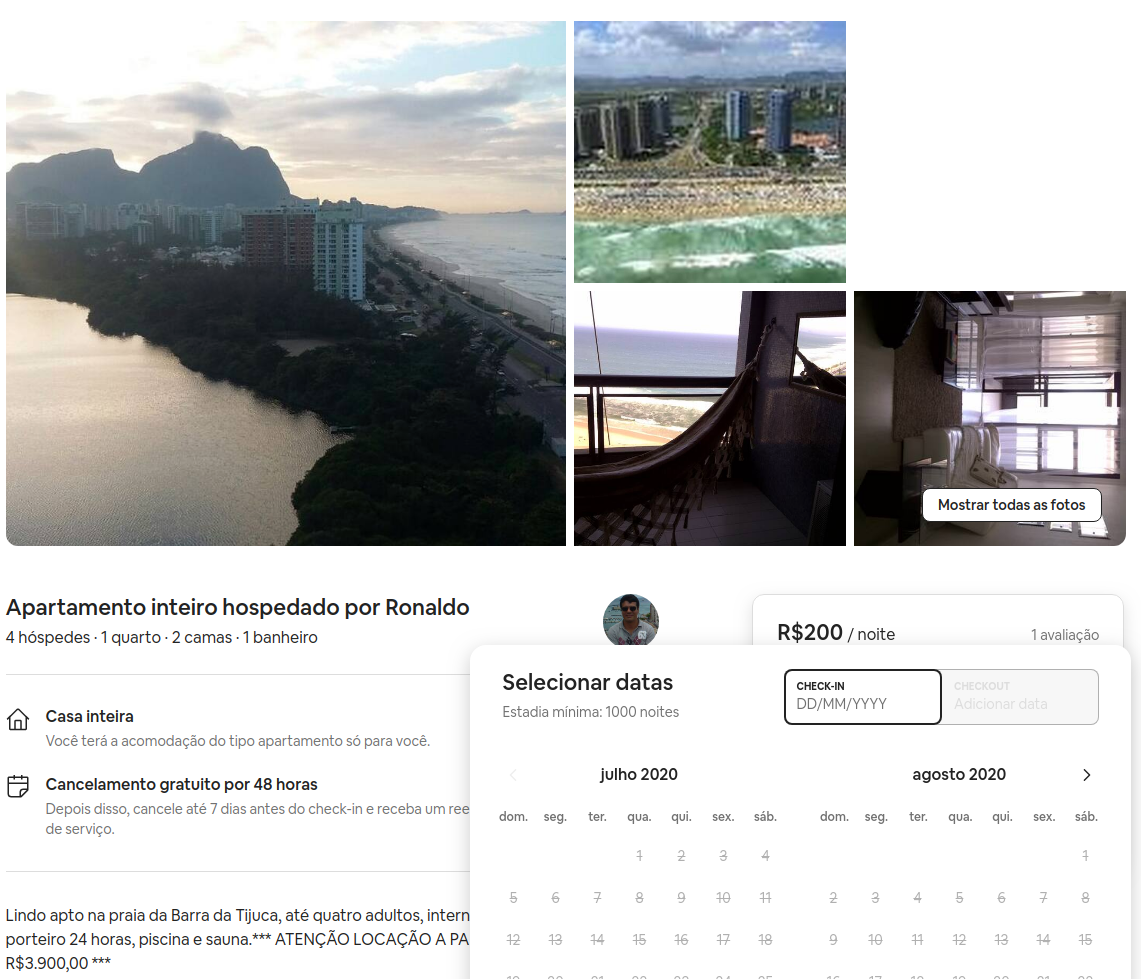
\includegraphics[width=\textwidth,height=0.5\textheight]{../fig/exemplo_periodo_airbnb.png}
\caption{Um exemplo de valor extremo de quantidade minima de
noites.\label{fig:minima_noites}}
\end{figure}

\hypertarget{apuxeandice-b}{%
\chapter*{APÊNDICE B}\label{apuxeandice-b}}
\addcontentsline{toc}{chapter}{APÊNDICE B}

O algoritmo abaixo realiza a otimização dos hiperparâmetros do Random
Forest.

\begin{algorithm}[H]
  \KwData{Base de Treino}
  \KwResult{Hiperparâmetros com menor erro}

  \SetKwProg{Pn}{Fun\c{c}ão}{:}{\Return erro}
      \Pn{TestaHiperparametros(folds, [hiperparâmetros])}{

        erro = [] \;

         \Para{i = 1 \textbf{ at\'{e} } 10}{
            train = PegaPartesdeTreino(folds, i)

            test = PegaPartedeTeste(folds, i)

            model = RandomForest(train, [hiperparâmetros])

            erro.append(EQM(model, test))
        }
    }

  folds = Separar a base em 10 partes para validação cruzada

  \Para{i = 1 \textbf{ at\'{e} } T}{
    \nosemic amostra = Gera uma amostra aleatória com 10 hiperparâmetros não testados

    TestaHiperparametros(folds, amostra)

    modelo = RandomForest(Hiperpar\^ametros testados, erro \sim hiperpar\^ametros)

    previsão = Prevê o valor do erro dos hiperpar\^ametros não testados

    amostra = Avalia o top 10 com menor previsão de erro

    TestaHiperparametros(folds, amostra)
  }

\caption{Algoritmo para encontrar um bom conjunto de hiperparâmetros}
\label{alg:hiper}
\end{algorithm}

% ----------------------------------------------------------
% ELEMENTOS PÓS-TEXTUAIS
% ----------------------------------------------------------
\postextual

% ----------------------------------------------------------
% Referências bibliográficas
% ----------------------------------------------------------
\bibliography{bibliography.bibtex}

\printindex

\end{document}
